\chapter{Classic Bayesian Decision Analysis} % Main chapter title

\label{chapter2} % For referencing the chapter elsewhere, use \ref{Chapter1} 

\lhead{Chapter 2. \emph{Classic Bayesian Decision Analysis}}



In the introduction we discussed the use of Bayesian reasoning and modelling techniques at the inception of probabilistic \glspl{ES}. Although we noted the inappropriateness of standard methodologies for the needs of current applications, several systems are still based on these traditional models. Furthermore, the theory we develop in the following chapters is a generalization of Bayesian methodologies and models to formally accommodate the beliefs of different group of experts. Therefore, we need to provide a broad overview of the currently available Bayesian modelling tools for \glspl{DM}. 

The chapter is structured as follows. In Section \ref{sec:bayesianreasoning} we outline the Bayesian formalism of inference, also defining moments and introducing Bayes linear methodology which only requires the specification of the first two moments. Section \ref{sec:SEU} introduces the \acrfull{SEU} model which embeds canons of rational decision making and defines rules to make decisions that are optimal according to these canons. The \gls{SEU} model basically consists of two main ingredients: a probability function, representing the beliefs of a \gls{DM}, and a utility function, representing her values. Sections \ref{sec:prob} and  \ref{sec:ut} introduce methodologies to represent respectively probability and utility functions having several arguments, i.e. in a multivariate setting. In such a case the definition and elicitation of these functions is often prohibitive. Independence concepts have been introduced to factorize these into subfunctions with a smaller number of arguments. Such factorizations can be often depicted by a graph providing a powerful and intuitive representation of the relationships between the elements of the problem. Therefore our discussion is mainly based on graphical models, for both probabilities and utilities.

In Section \ref{sec:dec} we introduce classes of models that explicitly represent both probabilities and utilities, and the decisions available to a single \gls{DM}. Again our discussion focuses on graphical models and in particular on the already mentioned \acrfull{ID} model.

The \gls{SEU} model is only capable of representing how a single \gls{DM} should rationally commit to decisions. However, as we have seen in Chapter \ref{chapter1}, policy choices are seldom made by just one person. There might be several \glspl{DM} sharing the authority and responsibility of choosing a certain policy, many stakeholders who are affected by the \gls{DM}'s decision, and experts that are consulted by the \gls{DM}. In Section \ref{sec:group} we review the literature on both group decision making and the use of expert judgement to support decision making. We then conclude with a discussion.

\section{Bayesian Reasoning}
\label{sec:bayesianreasoning}
\subsection{The Full Probabilistic Case}
A problem domain is denoted by an often large dimensional random vector
 $\bm{Y}$ taking values in the space $\bm{\mathcal{Y}}$. We denote with $\bm{y}$ a generic instantiation of $\bm{Y}$ and we let $\bm{\theta}\in\bm{\Theta}$ parametrize the density function $f$ of $\bm{Y}$. In a Bayesian framework the parameter $\bm{\theta}$ is itself a random variable and we let $\pi$ be its density function. For the purposes of this section, the vectors are assumed to be continuous\footnote{In discrete domains integrals are simply substituted by summations. We denote probability mass functions by $p$.}.  Let $\bm{X}$ be a random vector sampled from the same population as $\bm{Y}$ providing some data points $\bm{x}$. Within this framework, \textbf{Bayes theorem} can be  simply  employed to update the beliefs about $\bm{\theta}$ after the evidence $\bm{x}$ has been observed, as 
\begin{equation}
\label{eq:bayes}
\pi(\bm{\theta}\;|\;\bm{x})=\frac{f(\bm{x}\;|\;\bm{\theta})\pi(\bm{\theta})}{f(\bm{x})}=\frac{f(\bm{x}\;|\;\bm{\theta})\pi(\bm{\theta})}{\int_{\bm{\Theta}}f(\bm{x}\;|\;\bm{\theta})\pi(\bm{\theta})\dr \bm{\theta}}.
\end{equation}
The terms of equation (\ref{eq:bayes}) have all a meaning. The so called \textit{prior distribution} $\pi(\bm{\theta})$ represents the beliefs of the \gls{DM} about the parameter $\bm{\theta}$ before the evidence $\bm{x}$ is introduced into the system. If for example $\bm{Y}$ were a binary random variable, then $\pi(\bm{\theta})$ would simply be a probability distribution over $[0,1]$ representing the beliefs of the \gls{DM} about the probability of a success (for simplicity here we have chosen a discrete example). Although we do not further discuss these issues, we note that there is now an extensive literature and several software that allow for a faithful elicitation of such prior beliefs \citep[see for example][]{O'Hagan2006a}. The other term at the numerator, $f(\bm{x}\;|\;\bm{\theta})$, is usually called \textit{likelihood function}. In a Bayesian setting this measures the \gls{DM}'s degree of belief in the data taking certain values given that the parameter takes a certain hypothetical value. Continuing the example above, the likelihood would be in this situation the density of a Bernoulli random variable with a hypothetical unknown probability of success. The denominator of equation (\ref{eq:bayes}), $f(\bm{x})$,  simply corresponds to a normalizing constant, since for a Bayesian all the relevant information is related to $\bm{\theta}$. Therefore equation (\ref{eq:bayes}) is often presented in the following form,
\begin{equation}
\label{eq:proprbayes}
\pi(\bm{\theta}\;|\;\bm{x})\propto f(\bm{x}\;|\;\bm{\theta})\pi(\bm{\theta}),
\end{equation}
where $\propto$ corresponds to proportionality.  Furthermore, such a normalizing constant is often difficult to compute, since it requires an integration over an arbitrarily large space. Thus, equation (\ref{eq:proprbayes}) further represents a computationally less intensive version of (\ref{eq:bayes}). Finally, the posterior distribution $\pi(\bm{\theta}\;|\;\bm{x})$ is simply the revised density function of $\bm{\theta}$ after  evidence $\bm{x}$ has been observed. Assume for example that $\bm{x}$ in the running example is the result of ten coin tosses showing all head (or 1) and assume that the prior distribution was symmetric around 1/2. The posterior distribution would then be left-skewed and values in the interval $(1/2,1]$ would have in general higher probability than the ones in $[0,1/2]$. Henceforth we assume all these densities to represent the subjective Bayesian beliefs of a \gls{DM} \citep[for more details on the various interpretation of probabilities and the adequateness of the Bayesian interpretation in decision making, see for example ][]{O'Hagan2004a} and \citet{French2000b}.

Depending on whether the variables are continuous or discrete, on their support and  on the domain under study, there exist several different possible choices for both the likelihood function and the prior density. We review a variety of standard models in Appendix \ref{appendixE}, as for example the Bayesian normal linear model, which assumes a normal distribution for both the likelihood and the prior density of the mean when the variance is assumed to be known. We note here that a computationally efficient choice of prior and likelihood are of two that are \textit{conjugate} \citep{Bernardo2009, O'Hagan2004a}. This is the case whenever the posterior, computed via Bayes theorem, lies in the same family of distributions as the prior. In the example above if $\pi(\bm{\theta})$ were chosen to follow a Beta distribution with parameters $(a,b)\in\mathbb{R}^2_{>0}$, then the posterior would also be a Beta with some new parameters $(a^{'},b^{'})\in\mathbb{R}^2_{>0}$ (see Appendix \ref{sec:beta}).

Implicitly in equation (\ref{eq:bayes}) we assumed that the parameters of the distribution of $\bm{\theta}$ were known. Within the Bayesian approach this does not have to be necessarily the case and several different levels or layers of uncertainty can be introduced. This modelling strategy is usually referred to as multilevel or \textit{hierarchical modelling} \citep{Gelman2006}. For example, the parameters of the Beta distribution above, $a$ and $b$, could have been assumed to be random and depending on some other parameters, which could have further been random variables, and so forth. For the purposes of this thesis we only consider hierarchies consisting of one layer so that the parameters of $f(\bm{\theta})$ are known. These are usually referred to as \textit{hyperparameters}. 

\subsection{Moments}
Density functions can be easily summarized using the notion of \textit{moments}, which can describe some of their features. Moments are expected values of power functions of random variables. To introduce these, we first define the concept of expected  values. Let $g:\bm{\mathcal{Y}}\rightarrow \bm{\mathcal{Y}'}$, i.e. $g$ is a function mapping elements of $\bm{\mathcal{Y}}$ into $\bm{\mathcal{Y}'}$. 

\begin{definition}
\label{def:expectedvalue}
The expected value of $g(\bm{Y})$ is defined as\footnote{In the discrete case equations (\ref{eq:exp}) and (\ref{eq:condexp}) have a slightly different form which is not relevant for this thesis and can be found in \citet{Casella2002}.}
\begin{equation}
\label{eq:exp}
\E(g(\bm{Y}))=\int_{\bm{\mathcal{Y}'}}g(\bm{y})f(\bm{y})\dr \bm{y}=\int_{\bm{\Theta}}\E(g(\bm{Y})\;|\;\bm{\theta})\pi(\bm{\theta})\dr \bm{\theta},
\end{equation}
where the expected value $\E(g(\bm{Y})\;|\;\bm{\theta})$ conditional  on $\bm{\theta}$ is defined as
\begin{equation}
\label{eq:condexp}
\E(g(\bm{Y})\;|\;\bm{\theta})=\int_{\bm{\mathcal{Y}'}}g(\bm{y})f(\bm{y}\;|\;\bm{\theta})\dr\bm{y}.
\end{equation}
\end{definition}
For continuity with the previous section, we considered in Definition \ref{def:expectedvalue} quantities conditional on the parameter vector $\bm{\theta}$. However in general the conditioning might operate over any random vector of interest.

We can now define the notion of moment. Let for this purpose $\bm{s}\in \mathbb{Z}_{\geq 0}^n$, such that $\bm{s}=(s_1,\dots,s_n)^\T$, and let $\bm{Y}^{\bm{s}}=Y_1^{s_1}\cdots Y_n^{s_n}$. 

\begin{definition}
We say that the moment of order $\bm{s}$ of $\bm{Y}$ is $\E(\bm{Y}^{\bm{s}})$. The moment of order $\bm{s}$ of $\bm{Y}$ conditional on $\bm{\theta}$ is $\E(\bm{Y}^{\bm{s}}\;|\;\bm{\theta})$. The central moment and the central moment conditional on $\bm{\theta}$ of order $\bm{s}$ are defined respectively as $\E\left(\left(\bm{Y}-\E\left(\bm{Y}^{\bm{1}}\right)\right)^{\bm{s}}\right)$ and $\E\left(\left(\bm{Y}-\E\left(\bm{Y^{\bm{1}}\;|\;\bm{\theta}}\right)\right)^{\bm{s}}\;|\;\bm{\theta}\right)$, where $\bm{1}$ is a vector of dimension $n$ with $1$ in each entry.
\end{definition}

 We now define some specific moments.

\begin{definition}
Let $\bm{Y}$, $\bm{Y}_i$ and $\bm{Y}_j$ be  random vectors of dimension $n$. The expectation of $\bm{Y}$ is $\E(\bm{Y})=\E(\bm{Y}^{\bm{1}})$, whilst the variance of $\bm{Y}$, $\V(\bm{Y})$, is $\E((\bm{Y}-\E(\bm{Y}))(\bm{Y}-\E(\bm{Y}))^\T)$. The covariance between $\bm{Y}_i$ and $\bm{Y}_j$, $\Cov(\bm{Y}_i,\bm{Y}_j)$, is $\E((\bm{Y}_i-\E(\bm{Y}_i))(\bm{Y}_j-\E(\bm{Y}_j))^\T)$. 
\end{definition}

\begin{definition}
Let $\bm{Y}$, $\bm{Y}_i$ and $\bm{Y}_j$ be  random vectors of dimension $n$. The conditional expectation of $\bm{Y}$ given $\bm{\theta}$ is $\E(\bm{Y}\;|\;\bm{\theta})=\E(\bm{Y}^{\bm{1}}\;|\;\bm{\theta})$, whilst the conditional variance of $\bm{Y}$ given $\bm{\theta}$, $\V(\bm{Y}\;|\;\bm{\theta})$, is $\E((\bm{Y}-\E(\bm{Y}\;|\;\bm{\theta}))(\bm{Y}-\E(\bm{Y}\;|\;\bm{\theta}))^\T\;|\;\bm{\theta})$. The conditional covariance between $\bm{Y}_i$ and $\bm{Y}_j$ given $\bm{\theta}$, $\Cov(\bm{Y}_i,\bm{Y}_j\;|\;\bm{\theta})$, is $\E((\bm{Y}_i-\E(\bm{Y}_i\;|\;\bm{\theta}))(\bm{Y}_j-\E(\bm{Y}_j\;|\;\bm{\theta}))^\T\;|\;\bm{\theta})$.
\end{definition}
We now list some properties of these operators.
\begin{proposition}
\label{prop:propmom}
Let $\bm{Y}_i$, $\bm{Y}_j$, $\bm{Y}_k$ and $\bm{Y}_l$ be random vectors of dimension $n$. Further let $B_i$, $B_j$, $B_k$ and $B_l$ be $n\times n$ matrices with real entries, whilst $\bm{b},\bm{b}_{i},\bm{b}_{k}\in\mathbb{R}^n$. The following identities hold. 
\begin{align}
&\Cov(\bm{Y}_i,\bm{Y}_j\;|\;\bm{\theta})=\E\left(\bm{Y}_i\bm{Y}_j^\T\;|\;\bm{\theta}\right)-\E(\bm{Y}_i\;|\;\bm{\theta})\E(\bm{Y}_j\;|\;\bm{\theta})^\T\nonumber\\
&\E(B_i\bm{Y}_i\pm B_j\bm{Y}_j\pm \bm{b}\;|\;\bm{\theta})=B_i\E(\bm{Y}_i\;|\;\bm{\theta})\pm B_j\E(\bm{Y}_j\;|\;\bm{\theta}) \pm \bm{b},\label{eq:linexp}\\
&\V(B_i\bm{Y}_i \pm B_j\bm{Y}_j\pm \bm{b}\;|\;\bm{\theta})=B_i\V(\bm{Y}_i\;|\;\bm{\theta})B_i^\T+B_j\V(\bm{Y}_j\;|\;\bm{\theta})B_j^\T\pm 2B_i\Cov(\bm{Y}_i,\bm{Y}_j\;|\;\bm{\theta})B_j,\nonumber\\
&\Cov(B_i\bm{Y}_i - B_j\bm{Y}_j\pm \bm{b}_{i},B_k\bm{Y}_k - B_l\bm{Y}_l \pm \bm{b}_{k}\;|\;\bm{\theta})=B_i\Cov(\bm{Y}_i,\bm{Y}_k\;|\;\bm{\theta})B_k^\T-B_i\Cov(\bm{Y}_i,\bm{Y}_l\;|\;\bm{\theta})B_l^\T
-\nonumber\\ 
&\hspace{7.8cm} B_j\Cov(\bm{Y}_j,\bm{Y}_k\;|\;\bm{\theta})B_k^\T+B_j\Cov(\bm{Y}_j,\bm{Y}_l\;|\;\bm{\theta})B_l^\T.\nonumber
\end{align}
It then follows letting $[s]=\{1,\dots,s\}$ that, for $s\in\mathbb{Z}_{\geq 1}$, and $\bm{Y}_1,\dots,\bm{Y}_s$ vectors of dimension $n$,
\begin{equation} 
\V\left(\sum_{i\in[s]}B_i\bm{Y}_i\right)=\sum_{i\in[s]}^tB_i\V(\bm{Y}_i)B_i^\T+2\sum_{i\in[s]}\sum_{j\in[i-1]}B_i\Cov(\bm{Y}_i,\bm{Y}_j)B_j^\T,\nonumber
\end{equation}
where $B_i$, $i\in[s]$, is an $n\times n$ matrix.
\end{proposition}

The following proposition then links conditional and unconditional moments of order one and two.

\begin{proposition}
\label{prop:towerrules}
Let $\bm{Y}_i$ and $\bm{Y}_j$ be two random vectors. It holds that
\begin{align}
\E(\bm{Y}_i)&=\E(\E(\bm{Y}_i\;|\;\bm{\theta})),\label{eq:tower}\\
\V(\bm{Y}_i)&=\E(\V(\bm{Y}_i\;|\;\bm{\theta}))+\V(\E(\bm{Y}_i\;|\;\bm{\theta})),\label{eq:totalvariance}\\
\Cov(\bm{Y}_i,\bm{Y}_j)&=\E(\Cov(\bm{Y}_i,\bm{Y}_j\;|\;\bm{\theta}))+\Cov(\E(\bm{Y}_i\;|\;\bm{\theta}),\E(\bm{Y}_j\;|\;\bm{\theta}))\label{eq:totalcov}.
\end{align}
\end{proposition}
Equations (\ref{eq:tower})-(\ref{eq:totalcov}) are usually called \textit{tower rules} of moments. Specifically, equation (\ref{eq:tower}) is the tower rule of expectations, whilst equations (\ref{eq:totalvariance}) and (\ref{eq:totalcov}) are referred to as law of total variance and covariance respectively.
 \citet{Brillinger1969} generalized the identities (\ref{eq:tower})-(\ref{eq:totalcov}) and deduced a recursive formula to compute cumulants of any finite order. Cumulants can be thought of as a function of the moments, and vice versa. Many properties of random vectors can be more easily investigated using cumulants than moments \citep[see e.g.][]{Zwiernik2012}.
 
\subsection{Bayes Linear}
\label{sec:bayeslinear}
Bayes linear theory \citep{Goldstein2007} is an alternative approach to the quantification of uncertainty and updating of beliefs which is based on expectation, rather than probability, as a primitive and only requiring the elicitation of the first two moments of a random vector. This allows for both an honest belief specification in problems that are too complex to be dealt with  using standard Bayesian models and a computationally more efficient propagation of beliefs, since updating is based on simple linear fitting rather than conditioning. Here we provide a brief introduction of the main features of this approach.

We introduce here a notation we  extensively use throughout this thesis. Let, for $n\in\mathbb{Z}_{\geq 1}$, $[n]=\{1,\dots,n\}$ and $\bm{Y}=\bm{Y}_{[n]}^\T=(Y_1,\dots,Y_n)=(Y_i)_{i\in[n]}$, where $Y_i$ is a random variable. For a $B\subseteq[n]$, $\bm{Y}^\T_{B}=(Y_i)_{i\in B}$. For a partition $B$, $C$ of $[n]$, i.e. $B\cup C=[n]$ and $B\cap C=\emptyset$, let $\bm{Y}_C$ be the vector of variables the \gls{DM} plans to observe and $\bm{Y}_B$ the vector of variables she intends to modify her beliefs about.

\begin{definition}
The \textit{adjusted expectation} for $\bm{Y}_B$ given $\bm{Y}_C$, $\E_{\bm{Y}_C}^l(\bm{Y}_B)$ is defined as
\begin{equation}
\label{eq:adjexp}
\E_{\bm{Y}_C}^l(\Y_B)=\E(\Y_B)+\Cov(\Y_B,\Y_C)\V(\Y_C)^+(\Y_C-\E(\Y_C)),
\end{equation}
where $\V(\Y_C)^+$ is the Moore-Penrose generalized inverse of $\V(\Y_C)$ \citep[see e.g. Chapter 11 of][]{Goldstein2007}.
\end{definition}

 It is possible to show that the adjusted expectation is a linear operator just like the standard expectation as shown in equation (\ref{eq:linexp}). It is also clear that the adjusted expectation in (\ref{eq:adjexp}) is a simple linear function of $\Y_C$.
 
\begin{definition} 
The \textit{adjusted variance} for $\bm{Y}_B$ given $\bm{Y}_C$, $\V_{\Y_C}^l(\Y_B)$, is defined as
\begin{equation}
\label{eq:adjvar}
\V_{\Y_C}^l(\Y_B)=\V(\Y_B)-\Cov(\Y_B,\Y_C)\V(\Y_C)^+\Cov(\Y_C,\Y_B).
\end{equation}
\end{definition}
\begin{definition}
For a partition $B_i$, $B_j$ of $B$, we define the \textit{adjusted covariance} matrix between $\Y_{B_i}$ and $\Y_{B_j}$ given $\Y_C$, $\Cov_{\Y_C}^l\left(\Y_{B_i},\Y_{B_j}\right)$, as
\begin{equation}
\label{eq:adjcov}
\Cov_{\Y_C}^l\left(\Y_{B_i},\Y_{B_j}\right)=\Cov\left(\Y_{B_i},\Y_{B_j}\right)-\Cov\left(\Y_{B_i},\Y_{C}\right)\V(\Y_C)^+\Cov\left(\Y_C,\Y_{B_j}\right).
\end{equation}
\end{definition}

Equations (\ref{eq:adjexp})-(\ref{eq:adjcov}) define how updating is performed within a Bayes linear framework and mirrors the Bayes rule for probabilities of equation (\ref{eq:bayes}).

We next note that the following identities hold, which mirrors the tower rules of the full Bayesian approach specified in Proposition \ref{prop:towerrules}.
\begin{proposition}
\label{prop:linearrules}
For a partition $B$, $C$ of $[n]$, it holds that
$
\E(\Y_{B})=\E\left(\E_{\Y_C}(\Y_B)\right)$, $
\V(\Y_B)=\V_{\Y_C}(\Y_B)+\V\left(\E_{\Y_C}(\Y_B)\right)$ and 
$\Cov(\Y_C,\Y_B)=\Cov\left(\Y_C,\E_{\Y_C}(\Y_B)\right)$.
\end{proposition}

\section{The Subjective Expected Utility Model}
\label{sec:SEU}
In the previous section we introduce the Bayesian framework for reasoning about and modelling uncertainty. However the Bayesian approach further provides an axiomatic basis for decision making, which embodies canons of rationality, usually referred to as the \textbf{\gls{SEU}} model. Broadly speaking this consists of three main components:
\begin{itemize}
\item a decision space $\bm{\De}$ which includes the decisions $\bm{d}\in\bm{\De}$ available to the \gls{DM};
\item a probability density $f$ over the unknown state $\y\in \bm{\MY}$ of a vector of relevant random variables $\Y$;
\item a utility function $u(\bm{d},\bm{r}(\y,\bm{d}))$ describing the \gls{DM}'s preferences over some random vector $\bm{R}$, whose instantiation $\bm{r}=\bm{r}(\y,\bm{d})$ is a function of both $\bm{d}$ and $\y$, and takes values in $\bm{\Rs}$.
\end{itemize}

Having dealt with probability in Section \ref{sec:bayesianreasoning}, we now focus on the utility function.
\begin{definition}
\label{def:ut}
A utility function with arguments $\bm{d}$ and $\bm{r}$ is a real-valued function unique up to positive affine transformations, $u:\bm{\De}\bigtimes\bm{\Rs}\rightarrow \mathbb{R}$, such that 
\begin{equation*}
\label{eq:utility}
\forall \; (\bm{d}_i,\bm{r}_i), (\bm{d}_j,\bm{r}_j)\in \bm{\De}\bigtimes\bm{\Rs},\;\; u(\bm{d}_i,\bm{r}_i)\geq u(\bm{d}_j,\bm{r}_j) \Leftrightarrow (\bm{d}_i,\bm{r}_i) \succeq (\bm{d}_j,\bm{r}_j),
\end{equation*}
where  $(\bm{d}_i,\bm{r}_i) \succeq (\bm{d}_j,\bm{r}_j)$ means that the \gls{DM} perceives that $(\bm{d}_i,\bm{r}_j)$ is at least as good as $(\bm{d}_j,\bm{r}_j)$ and $\bigtimes$ is the Cartesian product.
\end{definition}
Note that in general utility functions only represent preference rankings and do not include any representation of the strength of these preferences. This is the reason way utilities are unique up to affine transformations, since these transformations do not change the preference order described by $\succeq$. Therefore utility functions are usually normalized so that they take values between 0 and 1, i.e. $u:\bm{\De}\bigtimes\bm{\Rs}\rightarrow [0,1]$. There have been some theoretical studies considering strength of preferences \citep[see e.g.][]{Argyris2014}, but these are not considered within this thesis. 

The study of utility functions dates back to the work of \citet{VonNeumann2007} which mostly concerned the theory of games. Throughout the following years, several different authors derived different constructions of the \gls{SEU} model based on different, but related, sets of axioms \citep{Anscombe1963,DeGroot2005,French2000b,Savage1972}.  We assume throughout the thesis that a set of axioms underpinning the \gls{SEU} model holds and that the \gls{DM} is able to elicit both a utility function and a probability distribution respecting one of these.

Now that utility functions have been introduced, we can show how the \gls{SEU} model combines probabilities and utilities to guide decision making. Decisions are ranked according to their associated expected utility.

\begin{definition}
Let $\bm{\mathcal{D}}$ be a decision space, $f$ a density function for a random vector $\bm{Y}$ parametrized by $\bm{\theta}$ and $u$ a utility function with arguments $\bm{d}\in \bm{\mathcal{D}}$ and $\bm{r}$. The \textbf{expected utility} of a decision $\bm{d}$, $\bar{u}(\bm{d})$, is defined as
\begin{align}
\label{eq:expectedut}
\bar{u}(\bm{d})=&\int_{\bm{\Theta}}\bar{u}(\bm{d}\;|\;\bm{\theta})\pi(\bm{\theta})\dr \bm{\theta},\\
\intertext{where}
\label{eq:expectedcondut}
\bar{u}(\bm{d}\;|\;\bm{\theta})=&\int_{\bm{\MY}}u(\bm{r},\bm{d})f(\y\;|\;\bm{\theta},\bm{d})\dr\y,
\end{align}
is the \textbf{conditional expected utility}.
\end{definition}
\begin{definition}
We say that a decision $\bm{d}^*\in\bm{\mathcal{D}}$ is \textbf{optimal} if $\bm{d}^{*}$ maximizes the expected utility, i.e.
\begin{equation}
\label{eq:maxut}
\bm{d}^*=\arg\max_{\bm{d}\in\bm{\De}}\bar{u}(\bm{d}).
\end{equation}
\end{definition}

A few important points need to be made here. First, we underline that the \gls{SEU} describes rational decision making of a single \gls{DM} and there is no clear extension of this model to groups of \glspl{DM} (see Section \ref{sec:group}). Second, the utility function, differently to value functions considered for example within \gls{RODOS}, are able by construction  to model attitudes towards risk \citep[see e.g.][]{Keeney1993a}. Lastly, we remark that the \gls{SEU} model falls within the class of normative approaches to decision making. From a set of axioms describing rationality, normative approaches are then able to produce a ranking of the available actions. However, there is a huge body of empirical literature which shows that people do not make decisions according to the \gls{SEU} model \citep{Tversky1974}. This observation led on one hand to the development of extensions of the model \citep[e.g. prospect theory,][]{Kahneman1979}, and on the other to a different use of normative models to support \glspl{DM} instead of automatically select optimal decisions. For example the \gls{SEU} model can be implemented into a \gls{DSS} in order to allow the \gls{DM} to explore the effects of her judgements on the ranking of the actions available to her.

Although equations (\ref{eq:expectedut}) and (\ref{eq:expectedcondut}) easily describes how expected utility can be computed, we note that in multivariate and dynamic settings the elicitation of both the utility function and the density function is often prohibitive. Therefore, several concepts of independence and different modelling strategies have been discussed in the literature. We  first review the methods developed for the density $f$ and after for the utility function $u$. Another difficulty arises because of the maximization in equation (\ref{eq:maxut}) when $\bm{\De}$ is high-dimensional. We  show in Section \ref{sec:dec} methods that allow to decompose the maximization to take place into smaller spaces and therefore be computationally simpler. 
   
\section{Probability Models}
\label{sec:prob}
We introduce in this section a variety of models that decompose a probability density $f$ into smaller dimensional (conditional) densities. Our discussion focuses on graphical models since these can more easily describe the qualitative features underlying a certain domain of interest, a property that results fundamental for the developments of this thesis. We first introduce in Section \ref{sec:condind} the notion of conditional independence which is at the basis of the decomposition generated by graphical models. We then review non-dynamic and dynamic models in Sections \ref{sec:nondym} and \ref{sec:dynmod} respectively. In Section \ref{sec:causality} we introduce the notion of statistical causality and explain its importance within Bayesian reasoning. We conclude with a discussion in Section \ref{sec:emu} of the use probabilistic emulators. These  describe through a probability density the outputs of a complex deterministic function arising for example from complex computer codes. 
 
For ease of notation we leave the dependence on the decision $\bm{d}$ implicit in this section. However, although not explicitly labelled, the results below need to hold for every possible decision in $\bm{\mathcal{D}}$.
 
\subsection{Conditional Independence}
\label{sec:condind}
We discussed in Chapter \ref{chapter1} that the concept of conditional independence introduced in \citet{Dawid1979} was one of the factors that lead to the definition of various graphical models and therefore to the modularization of statistical models. Although it can be generally thought as a tertiary operator - $\cdot \independent \cdot \;|\; \cdot$ - exhibiting a set of properties \citep[see e.g.][]{Dawid1993, Smith1989}, we only consider conditional independence between random variables and vectors. It is important to point out that recently \citet{Dawid2014} generalized the notion of conditional independence to include both non-stochastic and stochastic variables and termed it \textit{extended conditional independence}. This notion can allow for a simpler and more compact representation of the various irrelevances described for example by an \gls{ID}. 

For the purposes of this section, let $A$, $B$ $C$ and $D$ be disjoint subsets of $[n]$ and   $g$ denote a generic function.

\begin{definition}
We say that $\bm{Y}_A$ is independent $\bm{Y}_B$ given $\Y_C$, $\Y_A\independent \Y_B \;|\; \Y_C$, if 
$
f(\y_A,\y_B,\y_C)=f(\y_A\;|\;\y_C)f(\y_B,\y_C).
$
\end{definition}
 The conditional independence statement $\Y_A\independent \Y_B \;|\; \Y_C$ asserts that the only information to infer $\Y_A$ from $\Y_B$ and $\Y_C$ is from $\Y_C$.  \citet{Dawid1979} showed that the conditional independence operator has the following properties.
\begin{proposition}
\label{prop:semigraph}
It holds that:
\begin{enumerate}
\item $\Y_A\independent \Y_B \;|\;\Y_C \Longleftrightarrow \Y_B\independent \Y_A \;|\;\Y_C $;
\item $\Y_A\independent \Y_B \;|\;\Y_C \Longrightarrow g(\Y_A)\independent \Y_B \;|\;\Y_C$;
\item $\Y_A\independent \Y_B \;|\;\Y_C \Longrightarrow \Y_A\independent \Y_B \;|\;\Y_C, g(\Y_A)$;
\item $\Y_A\independent \Y_B \;|\;\Y_C$ and $\Y_A\independent\Y_D\;|\;\Y_B,\Y_C \Longleftrightarrow \Y_A\independent\Y_D,\Y_B\;|\;\Y_C$.
\end{enumerate}
\end{proposition}
We refer throughout the thesis to the condition in point 1 as the \textit{symmetry property}, whilst point 4 is usually referred to as \textit{strong decomposition}. These properties of conditional independence are usually called \textit{semi-graphoid axioms}.

Note that, although conditional independence is deeply linked to particular factorizations of densities, it is qualitative in nature and therefore easier to identify and justify.

\subsubsection{Context Specific Independence.}
The notion of conditional independence is only able to describe statements of the form $\Y_A\independent \Y_B \;|\;\Y_C $ holding for every instantiation $\bm{y}_C\in \bm{\MY}_C$, where $\bm{\MY}_C$ is the sample space of $\bm{Y}_C$. However often this does not have to be the case and a domain can exhibit some independences only for subspaces of the sample space. \textit{Context specific} independences are able to depict this more general scenario \citep{Boutilier1996}. 

\begin{definition}
Let $\bm{\MY}_D'$ be a subspace of $\bm{\MY}_D$, the sample space of $\bm{Y}_D$. We say that $\Y_A$ and $\Y_B$ are contextually independent given $\Y_C$ and context $\y_D\in\bm{\MY}_D'$ if
\begin{equation*}
f(\y_A,\y_B,\y_C,\y_D)=f(\y_A\;|\;\y_C,\y_D)f(\y_B,\y_C,\y_D), \hspace{1cm} \mbox{ if } \y_D\in\bm{\MY}_D'.
\end{equation*}
\end{definition} 

In Sections \ref{sec:tree} and \ref{sec:CEG} we introduce two classes of models that can graphically explicitly model this more general class of conditional independence statements. 
 
\subsubsection{Bayes Linear Sufficiency.} 
\label{sec:bayessuff}
The concept of conditional independence can be translated within the theory of linear Bayes rather straightforwardly and is defined as follows.
\begin{definition}
For a partition $A$, $B$, $C$ of $[n]$, we say that $\bm{Y}_C$ is Bayes linear sufficient for $\bm{Y}_A$ for adjusting $\bm{Y}_B$ if 
\begin{equation}
\E_{\bm{Y}_{C\cup A}}^l(\bm{Y}_B)=\E_{\bm{Y}_C}^l(\bm{Y}_B),
\end{equation}
and denote it with $\bci{\bm{Y}_A}{\bm{Y}_B}{\bm{Y}_C}$.
\end{definition}
It is easy to see the parallel between Bayes linear sufficiency and traditional conditional independence, since in the former case $\bm{Y}_A$ does not provide any information to predict the mean of $\bm{Y}_B$ once $\bm{Y}_C$ is known. \citet{Goldstein2007} further shows that Bayes linear sufficiency entertains the semi-graphoid axioms and therefore can be considered as a conditional independence operator. Note that if $\bci{\bm{Y}_A}{\bm{Y}_B}{\bm{Y}_C}$ then
\begin{equation}
\Cov(\bm{Y}_A,\bm{Y}_B)=\Cov(\bm{Y}_A,\bm{Y}_C)\V(\bm{Y}_C)^+\Cov(\bm{Y}_C,\bm{Y}_B).
\label{eq:covlin}
\end{equation}

\begin{comment}
We now list some useful properties for belief's updating that derive from Bayes linear sufficiency statements.
\begin{proposition}
\label{prop:linearproperties}
If $\bci{\bm{Y}_A}{\bm{Y}_B}{\bm{Y}_C}$ then
\begin{itemize}
\item $\E_{\bm{Y}_B}^l(\bm{Y}_A)=\E_{\bm{Y}_B}^l(\E_{\bm{Y}_C}^l(\bm{Y}_A))$;
\item $\V_{\bm{Y}_B}^l(\bm{Y}_A)=\V_{\bm{Y}_C}^l(\bm{Y}_A)+\V_{\Y_B}^l(\E_{\bm{Y}_C}^l(\bm{Y}_A))$;
\item $\V_{\bm{Y}_{B\cup C}}^l(\bm{Y}_A)=\V_{\bm{Y}_C}^l(\bm{Y}_A)$;
\item $\Cov(\bm{Y}_A,\bm{Y}_B)=\Cov(\bm{Y}_A,\bm{Y}_C)\V(\bm{Y}_C)^+\Cov(\bm{Y}_C,\bm{Y}_B)$;
\item $\Cov_{\bm{Y}_B}^l(\bm{Y}_A,\bm{Y}_C)=\Cov_{\bm{Y}_B}^l(\E_{\bm{Y}_C}^l(\bm{Y}_A),\bm{Y}_C)$;
\item $\Cov(\bm{Y}_A,\E_{\bm{Y}_C}^l(\bm{Y}_B))=\Cov(\bm{Y}_A,\bm{Y}_B)$.
\end{itemize}
\end{proposition}
\end{comment} 

\subsection{Non Dynamic Models}
The notions of conditional independence introduced in Section \ref{sec:condind} is now exploited to define various types of models in a non-dynamic framework, i.e. when there is no recursive updating through time of the involved probabilities. Let $\Y^\T=(Y_i)_{i\in[n]}$ be a vector of random variable with sample space $\bm{\mathcal{Y}}=\bigtimes_{i\in[n]}\mathcal{Y}_i$, where $\mathcal{Y}_i$ is the sample space of $Y_i$, $\bm{y}\in\bm{\mathcal{Y}}$ and $y_i\in\mathcal{Y}_i$, $i\in[n]$. Let $\bm{\theta}_A$ parametrize the (conditional) density of $\bm{Y}_A$ having sample space $\bm{\mathcal{Y}}_A=\bigtimes_{i\in A}\mathcal{Y}_i$, $A\subseteq [n]$. The parameter $\bm{\theta}_A$ takes values in $\bm{\Theta}_A$, $A\subseteq [n]$, and let $\bm{\theta}^\T=(\bm{\theta}_i)_{i\in[n]}$  be the parameter associated to the density of $\bm{Y}$ taking values in $\bm{\Theta}=\bigtimes_{i\in[n]}\bm{\Theta}_i$.

\label{sec:nondym}
\subsubsection{Independence Models.}
The simplest such non dynamic model is the so called \textit{independence model}.
\begin{definition}
\label{def:indmodel}
An independence model for $(\bm{Y},\bm{\theta})$ is such that $\independent_{i\in[n]} Y_i\;|\;\bm{\theta}$.
\end{definition} 
Such model class can be simply described by a graph with vertex set  $\{Y_i:i\in[n]\}$ and empty edge set.
 
\subsubsection{Bayesian Networks.}
\label{sec:BN}
\glspl{BN} \citep{Pearl1988a, Jensen2009, Korb2003, Lauritzen1996a, Smith2010} are the graphical model  most widely used  in practice. There are now thousands of applications of these probabilistic tools in a variety of domains \citep{Aguilera2011, Cowell2011,Heckerman1995, Niedermayer2008,Uusitalo2007}. These are especially attractive because the \gls{DAG} associated to a  \gls{BN} embodies qualitative information in terms of various conditional independences, and so often easier to elicit and explain then some of their competitors. Explicitly, in a \gls{BN} each random variable of the problem corresponds to a vertex of the \gls{DAG} and directed edges between vertices represent possible dependencies between the variables. 

 Only density functions associated to certain sets of conditional independences can be represented by a specific \gls{DAG} model. The following definition introduces one such class of conditional independence requirements. We let the set $A_i'\subset[n]$ consist of the indices of the ancestors of $Y_i$ minus $i$, whilst $\Pi_i\subset[n]$ consist of the indices of its parents, $i\in[n]$. 

\begin{definition}
A probability density $f$ over $\bm{Y}$ is said to obey the \textbf{local directed Markov property} relative to a \gls{DAG} $\Gr$, if, for $i\in[n]$, 
$\ci{Y_i}{\bm{Y}_{A_i'}}{\bm{Y}_{\Pi_i}}$.
\end{definition}

Therefore, a \gls{DAG} is able to describe the conditional independences of a random vector only if the associated density is local directed Markov. \citet{Cowell1999a}, among the others, showed that there are other equivalent statements to the local directed Markov property that can characterize probability densities respecting the topology of a \gls{DAG}. One such condition is the so called recursive factorization property of the density function. 
\begin{lemma}
\label{lemma:rec}
If a density $f$ over $\bm{Y}$ obeys the local directed Markov property relative to $\Gr$, then it respects the \textit{recursive factorization} formula, i.e.
\begin{equation*}
\label{eq:recursivefactorization}
f(\bm{y}\;|\; \bm{\theta})=\prod_{i\in[n]}f(y_i\;|\; \bm{y}_{\Pi_i}, \bm{\theta}_i)
\end{equation*}
\end{lemma}

The \gls{BN} model can now be formally defined as follows.
\begin{definition}
\label{def:BN}
A \gls{BN} over $\bm{Y}$ consists of 
\begin{itemize}
\item a \gls{DAG} $\Gr$ with vertex set $\{Y_i:i\in[n]\}$ and an edge from $Y_i$ to $Y_j$ iff $i\in \Pi_j$;
\item for $i\in[n]_1=[n]\setminus\{1\}$, the conditional independence statements of the form
$
\ci{Y_i}{\bm{Y}_{A_i'}}{\bm{Y}_{\Pi_i}}
$;
\item for $i\in[n]$, the conditional densities $f(y_i\;|\; \bm{y}_{\Pi_i}, \bm{\theta}_i)$.
\end{itemize}
\end{definition} 

As briefly pointed out previously, one of the main strengths of \gls{BN} modelling lies in its qualitative nature. Relationships between random variables are intuitively depicted by a graph, which are therefore easy to justify and explain in natural language. \citet{Smith2010} describes a protocol that can be followed to elicit the graph structure associated to a \gls{BN}, whilst \citet{OHagan2006} discusses how the associated densities can be quantified. Although in this thesis we always assume that the structure of the \gls{DAG} of a \gls{BN} is elicited by either a \gls{DM} or appropriate experts, we note here that several routines to automatically learn the \gls{DAG}'s topology from data are now in place under a variety of conditions \citep{Neapolitan2004, Cooper1999}.

\begin{figure}
\vspace{0.3cm}
\entrymodifiers={++[o][F-]}
\centerline{
\xymatrix{
\mbox{\large{$Y_4$}}&\mbox{\large{$Y_2$}}\ar[d]\\
\mbox{\large{$Y_1$}}\ar[u]\ar[ur]\ar[r]&\mbox{\large{$Y_3$}}
}
}
\vspace{0.3cm}
\caption{
Example of a  directed acyclic graph depicting the relationships between four random variables. \label{fig:BNexample}}
\end{figure}

\begin{example}
\label{example:BN}
Consider the \gls{DAG} in Figure \ref{fig:BNexample} with vertex set  $\{Y_1, Y_2, Y_3, Y_4\}$ and suppose
\begin{multicols}{2}
\begin{itemize}
\item $Y_1$: amount of contamination;
\item $Y_2$: human radioactive intake;
\item $Y_3$: effects on human health;
\item $Y_4$: political disruption.
\end{itemize}
\end{multicols}
The only conditional independence statement associated to the \gls{DAG} of Figure \ref{fig:BNexample}, is $\ci{Y_4}{Y_3,Y_2}{Y_1}$, implying that once the amount of contamination is known, human intake and effects on health are irrelevant to predict the political disruption. The recursive factorization associated to this \gls{DAG} corresponds to 
\begin{equation*}
\label{eq:BNexample}
f(y_1,y_2,y_3,y_4\;|\;\bm{\theta})=f(y_4\;|\;y_1,\bm{\theta}_4)f(y_3\;|\; y_2,y_1, \bm{\theta}_3)f(y_2\;|\; y_1,\bm{\theta}_2)f(y_1\;|\;\bm{\theta}_1).
\end{equation*}
\end{example}

The $n-1$ conditional independence statements that define a \gls{BN} model are not the only ones that are implied by a given model. The \textbf{D-separation} criterion \citep{Lauritzen1996a} provides a rule to verify whether or not a generic conditional independence statement holds for a \gls{BN} model. For three disjoint subsets $A$, $B$ and $C$ of $[n]$, the conditional independence $\ci{\bm{Y}_A}{\bm{Y}_B}{\bm{Y}_C}$ holds iff $\{Y_i:i\in C\}$ separates $\{Y_i:i\in A\}$ from $\{Y_i:i\in B\}$ in the moral graph of $\Gr$ (see Appendix \ref{appendixB}). Importantly, a set of conditional independence statements does not uniquely identify a \gls{DAG}: several \glspl{DAG} can represent the same set of conditional independences. Such \glspl{DAG} are said to be \textit{equivalent}. So for example, the \gls{DAG} in Figure \ref{fig:BNexample} would still imply the same conditional independence structure if the edge between $Y_2$ and $Y_3$ were reversed. We discuss in more details in Section \ref{sec:causality} how this issue is related to the concept of statistical causality.

We further note that the \gls{BN} model provides the basis for fast computation of probabilities through propagation techniques over the graph. The propagation is usually performed over the junction tree of the \gls{DAG} \citep[see e.g.][]{Smith2010}, but also other, often approximated, methodologies exist \citep{Murphy1999, Cowell1999a}.  \citet{Spiegelhalter1990} introduced two conditions over the parameter vector $\bm{\theta}$ that can allow for computations to be fast but still exact. The first one, equivalent to the strong directed hyper Markov condition of \citet{Dawid1993}, requires the parameters to be independent of each other. 
\begin{definition}
\label{def:global}
For a \gls{BN} over $\bm{Y}$ we say that $\bm{\theta}$  respects the \textbf{global independence} condition if 
$\independent_{i\in[n]} \bm{\theta}_i$.
\end{definition} 

The second condition concerns each parameter vector associated to a vertex.
\begin{definition}
Let $\bm{\theta}_i^\T=(\theta_{ji})_{j\in[n_i]}$, $n_i\in\mathbb{Z}_{\geq 1}$, $i\in[n]$. We say that the \textbf{local independence} condition holds if, for every $i\in[n]$,
$\independent_{j\in [n_i]^0}\theta_{ji}$, where $[n_i]^0=[n_i]\cup\{0\}$.
\end{definition}
Together local and global independence imply that the parameters are mutually independent of each other.

Note that the notion of global independence cannot hold unless the parameter spaces are \textit{variationally independent} \citep{Dawid2001,Dawid1993}. 
\begin{definition}
\label{def:varind}
 If $\bm{\Theta}=\bigtimes_{i\in[n]}\bm{\Theta}_i$ we say that thee spaces $\bm{\Theta}_1,\dots,\bm{\Theta}_n$ are variationally independent.
\end{definition}

Under the global independence assumption the following result hold.
\begin{proposition}
\label{prop:BNasDDM}
If global independence holds for a \gls{BN} with vertex set $\{Y_i:i\in[n]\}$, then
\begin{equation*}
f(\bm{y})=\int_{\bm{\Theta}}f(\bm{y},\bm{\theta})\dr \bm{\theta}=\int_{\bm{\Theta}}\prod_{i\in[n]}f(y_i\;|\;\bm{y}_{\Pi_i},\bm{\theta}_i)\pi(\bm{\theta}_i)\dr\bm{\theta} =\prod_{i\in[n]}f(y_i\;|\;\bm{y}_{\Pi_i}),
\end{equation*}
where
\begin{equation*}
f(y_i\;|\;\bm{y}_{\Pi_i})=\int_{\bm{\Theta}_i}f(y_i\;|\;\bm{y}_{\Pi_i},\bm{\theta}_i)\pi(\bm{\theta}_i)\dr\bm{\theta}_i.
\end{equation*}
\end{proposition}
Therefore under the assumption of global independence also the marginal distribution over $\bm{Y}$ factorizes according to the underlying \gls{DAG}. This is general would not be true without this assumption.

Also Bayesian updating given a sample $\bm{x}$ can be performed in a distributed fashion under the global independence assumption. The sample $\bm{x}$ does not need to be complete in order for this to be the case as the following proposition formalizes. We let $Fa_i\subseteq[n]$ and $De_i\subset[n]$ be the index sets of the family and the descendants of $Y_i$, $i\in[n]$.

\begin{proposition}
\label{prop:ancupd}
Suppose $\bm{x}$ is an ancestral sample from the same population of $\bm{Y}$, meaning that if $\bm{x}_i$, the sample relative to $Y_i$, is observed, then $\bm{x}_{A_i'}$ is observed as well. Then, if global independence holds and letting $I$ be the set of indices of the vertices whose children are not sampled, we have that
\begin{equation*}
\pi(\bm{\theta}\;|\;\bm{x})=\prod_{l\in I}\prod_{j\in A_l}\pi(\bm{\theta}_j\;|\;\bm{x}_{Fa_j})\prod_{k\in De_l}\pi(\bm{\theta}_k).
\end{equation*}
\end{proposition}
Similar recursions hold for local independence as well which retain the independence of the parameters a posteriori \citep[see][]{Spiegelhalter1990}.

We next consider \glspl{GBN}, which define a Gaussian distribution for the random vector $\bm{Y}$ respecting the conditional independences implied by a \gls{DAG}. Specifically, given a \gls{DAG} $\Gr$, it is possible to associate to each vertex a normal distribution through a simple linear regression. For this purpose, let for , $i\in[n]$, $j\in[n]_i$, where $[n]_i=[n]\setminus [i]$,
\begin{equation}
\label{eq:GausBN}
Y_i=\theta_{0i}+\sum_{j\in \Pi_i} \theta_{ji}Y_j+\varepsilon_i, 
\end{equation} 
with $\theta_{ji}\in\mathbb{R}$ regression parameters and  errors $\varepsilon_i\sim (0,\psi_i)$, meaning that these have mean zero and variance $\psi_i$, independent of each other and of the $Y_j$'s. If $\varepsilon_i$, $i\in[n]$, is further assumed to be normal, we say that equation (\ref{eq:GausBN}) is a \textit{Gaussian linear regression}. The following proposition, from \citet{Richardson2002}  and expressed here in the form of \citet{Sullivant2010}, then shows how to build a multivariate normal distribution from these regression specifications respecting the conditional independence statements associated to the graph.
\begin{proposition}
\label{proposition:ciao2}
Let $\bm{Y}^\T=(Y_i)_{i\in[n]}$ be a random vector, where each $Y_i$ is defined as a  Gaussian linear regression. Let $\Psi=diag(\psi_1,\dots, \psi_n)$ and $L$ be an upper triangular $n\times n$ matrix defined as
\begin{equation*}
\label{eq:Lji}
L_{ji}=\left\{
\begin{array}{ll}
\theta_{ji},& \mbox{if } j\in \Pi_i\\
0,&\mbox{otherwise.}
\end{array}
\right.
\end{equation*}
Define $B=I_n-L$, where $I_n$ is the $n\times n$ identity matrix, and $\bm{\theta}_0^\T=(\theta_{0i})_{i\in[n]}$. Then it holds that $\bm{Y}\sim N\left({(B^{-1})}^\T\bm{\theta}_0,{(B^{-1})}^\T\Psi B^{-1} \right)$, where $N$ denotes a Gaussian random variable. 
\end{proposition} 

In a full Bayesian framework prior distributions for the regression parameters $\theta_{ji}$ and the error variances $\psi_i$ need to be further provided, as, for example, the normal-inverse gamma for the simple linear model shown in Appendix \ref{sec:nig}. We note here that although we have assumed each vertex to be a univariate random variable, this does not have to be the case in general. In such a situation a Normal-inverse Wishart prior distribution can be defined as shown in Appendix \ref{sec:niw}. 

In order to illustrate the notions of global and local independence for \glspl{GBN}, let $\bm{\theta}_i^\T=(\theta_{0i},\psi_i, \theta_{ji})_{j\in\Pi_i}$, $i\in[n]$. Global independence is then such that $\independent_{i\in[n]}\bm{\theta}_i$. Local independence on the other hand assumes that every element of a vector $\bm{\theta}_i$ is independent of the rest. 

\begin{comment}
\noindent
\textbf{Multinomial models.}
Assume each variable $Y_i$ is discrete and takes values in the space $\mathcal{Y}_i=\{0,\dots,r_i-1\}$. Let the conditional probability that $Y_i$ takes value $j\in\mathcal{Y}_i$ given that $\bm{Y}_{\Pi_i}=\bm{\pi}_i$ be equal to $\theta_{j\bm{\pi}_i}$. Then $Y_i\;|\;\bm{Y}_{\Pi_i}\sim Multi(\bm{\theta}_{i\bm{\pi}_i})$, where $\bm{\theta}_{i\bm{\pi}_i}^\T=(\theta_{j\bm{\pi}_i})_{j\in\mathcal{Y}_i}$. This is an instance of the contingency table model of Appendix \ref{appendixE13}, where in this case though the entries are conditional probabilities. Let $\bm{\theta}_i^\T=\left(\theta_{i\bm{\pi}}^\T\right)_{\bm{\pi}\in\mathcal{Y}_{\Pi_i}}$. Then global independence in this setting entails that $\independent_{i\in[n]}\bm{\theta}_i$, whilst from local independence it follows $\independent_{\bm{\pi}_i\in\mathcal{Y}_{\pi_i},j\in\mathcal{Y}_i}\theta_{j\bm{\pi}_i}$. 

Under the assumptions of local and global independence each $\bm{\theta}_{i\bm{\pi}_i}$ can be given an independent Dirichlet prior distribution and Bayesian updating can be performed locally for each of these parameters using the recursions shown in Appendix \ref{sec:multidir} when data comes from ancestral samples as formalized in Proposition \ref{prop:ancupd}.
\end{comment}
\noindent 
\subsubsection{Object Oriented Bayesian Networks.}
In complex large \glspl{BN}, identical subnetworks are often repeated in different parts of the \gls{DAG}. This is for example the case for the \gls{DAG} in Figure \ref{fig:BNwithsubs}, where the subnetworks within the two rectangles have the same topology. Now assuming that $Y_i'$ and $Y_i''$, $i\in [6]_1$, have the same sample space and equal conditional probability densities, we can then represent the network as an \gls{OOBN}. As extensively discussed in Chapter \ref{chapter1}, the object oriented paradigm has proven to provide a convenient framework to represent complex problems. We do not provide here a formal definition of this class of models \citep[which can be found in][]{Koller97} since it is beyond the scope of the thesis and would require the introduction of a rather intricate notation, but following \citet{Jensen2006} and \citet{Neil2000} we provide an intuitive example to describe their workings.
 
\begin{figure}
\begin{minipage}[b]{.65\linewidth}
\begin{center}
\begin{tikzpicture}[node distance=4cm]
\node[draw,circle] (30) at (3,0) {$Y_1'$};
\node[draw,circle](11) at (1,-1.5) {$Y_2'$};
\node[draw,circle] (51) at (5,-1.5) {$Y_2''$};
\node[draw,circle] (02) at (0,-3) {$Y_3'$};
\node[draw,circle] (22) at (2,-3) {$Y_4'$};
\node[draw,circle] (42) at (4,-3) {$Y_3''$};
\node[draw,circle] (62) at (6,-3) {$Y_4''$};
\node[draw,circle] (03) at (0,-4.5) {$Y_5'$};
\node[draw,circle](23) at (2,-4.5) {$Y_6'$};
\node[draw,circle](43) at (4,-4.5) {$Y_5''$};
\node[draw,circle] (63) at (6,-4.5) {$Y_6''$};
\node[draw,circle] (34) at (3,-6) {$Y_7$};
\draw[->] (30) -- (11);
\draw[->] (30) -- (51);
\draw[->] (11) -- (02);
\draw[->] (11) -- (22);
\draw[->] (51) -- (42);
\draw[->] (51) -- (62);
\draw[->] (02) -- (22);
\draw[->] (02) -- (03);
\draw[->] (22) -- (23);
\draw[->] (42) -- (62);
\draw[->] (42) -- (43);
\draw[->] (62) -- (63);
\draw[->] (63) -- (34);
\draw[->] (03) -- (34);
\draw[->] (03) -- (23);
\draw[->] (43) -- (63);
\node[draw=black, rounded corners=6pt, inner sep =7pt, fit=(11) (03) (23)] {};
\node[draw=black, rounded corners=6pt, inner sep =7pt, fit=(51) (43) (63)] {};
\end{tikzpicture}
\end{center}
\subcaption{Example of a Bayesian network with identical subnetworks. \label{fig:BNwithsubs}}
\end{minipage}
\begin{minipage}[b]{0.33\linewidth}
\begin{center}
\begin{tikzpicture}[node distance=4cm]
\node[draw,circle,dashed] (10) at (1,0) {$Y$};
\node[draw,circle] (11) at (1,-1.5) {$Y_2$};
\node[draw,circle] (02) at (0,-3) {$Y_3$};
\node[draw,circle] (22) at (2,-3) {$Y_4$};
\node[draw,circle,fill = black!30!white] (03) at (0,-4.5) {$Y_5$};
\node[draw,circle,fill = black!30!white] (23) at (2,-4.5) {$Y_6$};
\draw[->] (10) -- (11);
\draw[->] (11) -- (02);
\draw[->] (11) -- (22);
\draw[->] (02) -- (22);
\draw[->] (02) -- (03);
\draw[->] (22) -- (23);
\draw[->] (03) -- (23);
\node[draw=black, rounded corners=6pt, inner sep =7pt, fit=(10) (03) (23)] {};
\end{tikzpicture}
\end{center}
\subcaption{Class definition for the subnetworks of Figure \ref{fig:BNwithsubs}. \label{fig:class}}
\end{minipage}
\caption{Example of object orientation in Bayesian networks. \label{fig:objectorient}}
\end{figure}

Considering again the network in Figure \ref{fig:BNwithsubs}, each subnetwork within the rectangles in the object oriented paradigm is called  \textit{class} and each instantiation of a class is called  \textit{object}. Figure \ref{fig:class} shows the class definition for the repeated subnetworks of Figure \ref{fig:BNwithsubs}. Each class consists of three types of vertices:
\begin{itemize}
\item input vertices: not true random variables, but artificial nodes that serve as "placeholders". In Figure \ref{fig:class} the input vertex is the dashed node $Y$ which must have the same state space of $Y_1$;
\item encapsulated vertices: vertices that are hidden outside of the class and that are used only within the class. In Figure \ref{fig:class} the internal vertices are $Y_2$, $Y_3$ and $Y_4$;
\item output vertices: part of the class that is accessible from outside and that can be connected to other classes. The output vertices of the class in Figure \ref{fig:class} are the shaded nodes $Y_5$ and $Y_6$. 
\end{itemize}
Encapsulated and output vertices are allowed to be objects, whilst input vertices must be variables. 

Given the class definition in Figure \ref{fig:class}, we can represent the \gls{BN} of Figure \ref{fig:BNwithsubs} as the \gls{OOBN} reported in Figure \ref{fig:OOBN}.  In this network the encapsulated vertices are hidden and only input and output nodes of the class explicitly appear. Each rectangle is an object and in each object the relative output nodes are connected to elements external to the class. The dashed arrows into the input node indicate which node $Y$ is a placeholder for (in this case $Y_1$ for both objects).

Even in this simple example the expressive power of \glspl{OOBN} becomes apparent, modularizing the overall problem in different layers formally separated. Of course in much larger examples \glspl{OOBN} provides an even more compact representation of the domain under consideration: see for example \citet{Neil2000}.

\begin{figure}
\begin{center}
\begin{tikzpicture}[node distance=4cm]
\node[draw,circle] (30) at (3,0) {$Y_1$};
\node[draw,circle,dashed](11) at (1,-1.5) {$Y$};
\node[draw,circle,dashed] (51) at (5,-1.5) {$Y$};
\node[draw,circle,fill = black!30!white] (03) at (0,-3) {$Y_5$};
\node[draw,circle,fill = black!30!white](23) at (2,-3) {$Y_6$};
\node[draw,circle,fill = black!30!white](43) at (4,-3) {$Y_5$};
\node[draw,circle,fill = black!30!white] (63) at (6,-3) {$Y_6$};
\node[draw,circle] (34) at (3,-4.5) {$Y_7$};
\draw[dashed,->] (30) -- (11);
\draw[dashed,->] (30) -- (51);
\draw[->] (03) -- (34);
\draw[->] (63) -- (34);
\node[draw=black, rounded corners=6pt, inner sep =7pt, fit=(11) (03) (23)] {};
\node[draw=black, rounded corners=6pt, inner sep =7pt, fit=(51) (43) (63)] {};
\end{tikzpicture}
\end{center}
\caption{Object-oriented representation of the Bayesian network of Figure \ref{fig:BNwithsubs}, whose class is defined in Figure \ref{fig:class}. \label{fig:OOBN}}
\end{figure}

\subsubsection{Probabilistic Undirected Graphs.}
We now consider probability densities $f$ that can be described by an \gls{UG} $\Gr$. For the purposes of the thesis we assume $\Gr$ to be always decomposable in the undirected case: we  motivate this assumption below. Similarly to the directed case of Section \ref{sec:BN}, we first introduce a class of densities which are in some sense compatible to the graph and then define the class of \gls{UG} models called \textit{\acrfull{MN}}. References about these models are countless \citep[see e.g.][]{Lauritzen1996a, Cowell1999a, Castillo1997b} and we follow here \citet{Dawid1993}.

\begin{definition}
Let $A,B\subset[n]$ and $V(\Gr)=\{Y_i: i\in[n]\}$ be the vertex set of an \gls{UG} $\Gr$. A density $f$ over $\bm{Y}$ is called \textit{Markov} if, for any decomposition $\{Y_i:i\in A\}$, $\{Y_i:i\in B\}$ of $\Gr$,
$\bm{Y}_A\independent \bm{Y}_B \;|\; \bm{Y}_{A\cap B}$
\end{definition}

\begin{definition}
A decomposable \gls{MN} model consists of a decomposable \gls{UG} $\Gr$ with vertex set $\{Y_i:i\in[n]\}$ together with a Markov density $f$. 
\end{definition}
Note that for each vertex $Y_i$ of a \gls{MN}, the conditional independence statement
\begin{equation*}
\label{eq:independenceUG}
Y_i\independent \bm{Y}_{[n]\setminus \{i\}}\;|\; \bm{Y}_{Ne_i},
\end{equation*}
holds, where $Ne_i$ is the index set of the neighbours of $Y_i$. Thus, similarly to the directed case, Markov densities associated to a (decomposable) \gls{UG} are the only ones entertaining the separations implied by the graph. In order to deduce the associated Markov factorization as in the directed case, we first need to introduce the notion of \textit{consistency}.
\begin{definition}
Let $f_A$ and $f_B$ be densities over $\bm{Y}_A$ and $\bm{Y}_B$ respectively, $A,B\in[n]$. We say that $f_A$ and $f_B$ are consistent if they both yield the same density over $\bm{Y}_{A\cap B}$. 
\end{definition}
Now letting $\mathcal{C}$ and $\mathcal{S}$ be the sets of the indices of the cliques and the separators respectively of an \gls{UG} $\Gr$, we have the following.
\begin{lemma}
\label{lemma:Markov}
The unique Markov density $f$ over a decomposable \gls{UG} $\Gr$ having consistent densities as its clique marginals factorizes as
\begin{equation*}
\label{eq:UGmarkovfactorization}
f(\bm{y}\;|\;\bm{\theta})=\frac{\prod_{C\in\mathcal{C}}f(\bm{y}_C\;|\;\bm{\theta}_C)}{\prod_{S\in\mathcal{S}}f(\bm{y}_S\;|\; \bm{\theta}_S)^{v_S}},
\end{equation*}
where $v_S$ is the multiplicity of the separator $S$ and $\bm{\theta}_C$, $\bm{\theta}_S$ are the parameter vectors associated to $\bm{Y}_C$ and $\bm{Y}_S$ respectively.
\end{lemma} 

Given an order of the elements of $\mathcal{C}$ exhibiting the running intersection property, the density of a Markov density over a decomposable graph can be alternatively written as, assuming the graph includes $m$ cliques,
\begin{equation*}
\label{eq:cliquesfactorization}
f(\bm{y}\;|\;\bm{\theta})=\prod_{i\in[m]_1} f(\bm{y}_{R_i}\;|\; \bm{y}_{S_i}, \bm{\theta}_{R_i})f(\bm{y}_{C_1}),
\end{equation*}
where $R_i=C_i\setminus S_i$.

A short note on non decomposable \glspl{MN}: for these models there is no unique factorization in terms of probability densities, but only in terms of \textit{potentials}, i.e. generic positive functions. In general we have (without explicitly denoting the dependence on the parameters) 
\begin{equation*}
\label{eq:nondecomposable}
f(\bm{y})=\prod_{C\in\mathcal{C}}\phi(\bm{y}_C),
\end{equation*}
but these potentials $\phi$ have no clear physical meaning. This is one of the reasons why non-decomposable models are not particularly convenient to work with. In the following we provide a further evidence, specific for Bayesian analyses, to support this statement. 

\begin{figure}
\begin{center}
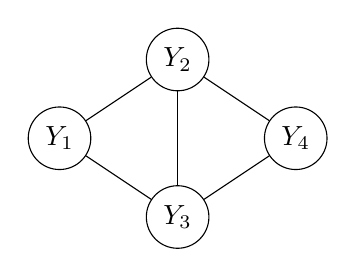
\begin{tikzpicture}
\node[draw,circle] (01) at (0,-1) {$Y_1$};
\node[draw,circle]  (10) at (1.5,0) {$Y_2$};
\node[draw,circle]   (12) at (1.5,-2) {$Y_3$};
\node[draw, circle]  (21) at (3,-1){$Y_4$};
\draw[-] (01) -- (10);
\draw[-] (01) -- (12);
\draw[-] (10) -- (12);
\draw[-] (21) -- (10);
\draw[-] (21) -- (12);
\end{tikzpicture}
\end{center}
\caption{Example of a decomposable undirected graph with four vertices. \label{fig:UG}}
\end{figure}

\begin{example}
Consider the \gls{UG}  with vertex set $\{Y_1,Y_2,Y_3,Y_4\}$ in Figure \ref{fig:UG}. The conditional independence statement associated to this graph is $
\ci{Y_4}{Y_1}{Y_2,Y_3}$,
and therefore the associated density factorizes as
\begin{equation*}
\label{eq:UGexamplefactorization}
f(\bm{y}\;|\;\bm{\theta})=\frac{f(y_1,y_2,y_3\;|\; \bm{\theta}_{123})f(y_2,y_3,y_4\;|\; \bm{\theta}_{234})}{f(y_2,y_3\;|\; \bm{\theta}_{23})},
\end{equation*}
or alternatively as
\begin{equation*}
\label{eq:UGexamplefactorization2}
f(\bm{y}\;|\;\bm{\theta})=f(y_4\;|\; y_2,y_3, \bm{\theta}_4)f(y_1,y_2,y_3\;|\; \bm{\theta}_{123})=f(y_1\;|\; y_2,y_3, \bm{\theta}_1)f(y_2,y_3,y_4\;|\; \bm{\theta}_{234}),
\end{equation*}
where $\bm{Y}^\T=(Y_i)_{i\in[4]}$ and $\bm{\theta}_{123}$, $\bm{\theta}_{234}$ and $\bm{\theta}_{23}$ are a shorthand of $\bm{\theta}_{[3]}$, $\bm{\theta}_{[4]_1}$ and $\bm{\theta}_{[3]_1}$ respectively.
\end{example}

Similarly to the directed case, conditions over the distribution of the parameters can be imposed to allow for distributed computing and inference. For the purposes of this thesis we introduce only the strong hyper Markov condition of \citet{Dawid1993}.
\begin{definition}
\label{def:strongMarkov}
A density $\pi$ is strong hyper Markov for $\Gr$ if, for any decomposition $\{Y_i:i\in A\}$, $\{Y_i:i\in B\}$ of $\Gr$, $\bm{\theta}_A\independent \bm{\theta}_B$.
\end{definition} 
Since the cliques of a decomposable \gls{UG} can be ordered to sequentially form a decomposition, we have the following result.
\begin{lemma}
\label{lemma:strongMarkov}
If a density $\pi$ for $\bm{\theta}$ is strong hyper Markov  then 
$
\pi(\bm{\theta})=\prod_{C\in\mathcal{C}}\pi(\bm{\theta}_{C}).$
\end{lemma}
We do not show in details how to build a distribution exhibiting the strong hyper Markov condition, but we briefly note here that this can be straightforwardly done by considering the Markov combinations \citep{Massa2010} of the marginal distributions over the cliques of the graph. 

The following proposition then shows how the strong hyper Markov condition is associated to fast distributed Bayesian inference.
\begin{proposition}
\label{prop:markovupdating}
Assume a vector $\bm{X}$ is sampled from the same population of $\bm{Y}$ and assume the density $\pi$ of $\bm{\theta}$ is strong hyper Markov. Then
\begin{itemize}
\item the posterior distribution obtained by conditioning on the complete data $\bm{X}=\bm{x}$ is strong hyper Markov;
\item the posterior distribution is the unique strong hyper Markov distribution specified by the clique-marginal prior distributions given by $
\pi(\bm{\theta}_C\;|\; \bm{x})=f(\bm{x}_C\;|\;\bm{\theta}_C)\pi(\bm{\theta}_C).$
\end{itemize}
\end{proposition}
Therefore Bayesian updating can be performed locally within each clique, whilst retaining the strong hyper Markov condition. Furthermore, this result implies that the family of strong hyper Markov distributions are conjugate with likelihoods that are Markov. Other conditions over the parameter vectors can be shown to be conjugate with Markov likelihoods, but these do not allow for local updating of probabilities. In addition the above result does not hold in general for non-decomposable undirected models: thus inference through local computations cannot be performed in such models. Importantly also note that, whilst global independence is retained after observing certain incomplete datasets, strong hyper Markov laws are broken by any incomplete observation. 

We now consider a specific class of \gls{MN} models whose associated distribution is Gaussian. A Gaussian \gls{MN} with decomposable \gls{UG} $\Gr$, $V(\Gr)=\{Y_i:i\in[n]\}$, is defined as $\bm{Y}\sim N(\bm{\mu},\Sigma)$, where $\bm{\mu}^\T=(\mu_i)_{i\in[n]}\in\mathbb{R}^n$ and $\Sigma$ is a positive semidefinite $n\times n$ matrix such that $
(Y_i,Y_j)\not\in E(\Gr)\Longrightarrow \Sigma_{ij}^{-1}=0$,
where $\Sigma_{ij}^{-1}$ is the entry of $\Sigma^{-1}$ in position $(i,j)$. So for example the covariance matrix associated to the Gaussian \gls{MN} with graph in Figure \ref{fig:UG} is such that its inverse has zero entries in position $(1,4)$ and $(4,1)$.
\begin{comment}
\begin{equation}
\left(
\begin{array}{cccc}
\sigma_{11}&\sigma_{21}&\sigma_{31}&0\\
\sigma_{21}&\sigma_{22}&\sigma_{32}&\sigma_{42}\\
\sigma_{31}&\sigma_{32}&\sigma_{33}&\sigma_{43}\\
0&\sigma_{42}&\sigma_{43}&\sigma_{44}
\end{array}
\right)^{-1}.
\end{equation}
\end{comment}
Now for simplicity let $\bm{\mu}=\bm{0}$. Such model class is usually referred to as covariance selection model \citep{Wermuth1976}. Recall from Appendix \ref{sec:niw} that the Inverse Wishart distribution allows for conjugate learning with normal models when defined as a prior of the covariance matrix. Let $\Sigma\sim IW(A,d)$, where $A$ is positive semidefinite $n\times n$ matrix and $d\in\mathbb{Z}_{\geq n}$. It is well known that for a subset $B\in[n]$, $\bm{Y}_{B}\sim N(\bm{0},\Sigma_{BB})$ and $\Sigma_{BB}\sim IW(A_{BB},d)$, where, for a matrix $\Sigma$, $\Sigma_{BB}$ is its submatrix with rows and columns $i\in B$ \citep[see e.g.][]{Dawid1993}. Let for every clique $C\in\mathcal{C}$ of $\Gr$, $\bm{Y}_{C}\sim N(\bm{0},\Sigma_{CC})$ and assume the covariance has an inverse Wishart prior $IW(A^C,d)$. A unique strong hyper Markov for the whole graph $\Gr$ having as marginals over the cliques these inverse Wishart distributions exists if, calling $S_{ij}=C_i\cap C_j$, the matrices $A^{C_i}_{S_{ij}S_{ij}}$ and $A^{C_j}_{S_{ij}S_{ij}}$ are identical.\footnote{This result follows from Proposition 5.9 of \citet{Dawid1993} which we have not introduced here since it would require the introduction of additional concepts not relevant for the thesis. In a nutshell, this result is true because the Inverse Wishart is conjugate for the normal covariance model and this distribution is a member of the exponential family.} We then say that $\Sigma$ follows an hyper Inverse Wishart distribution with parameters $A$ and $d$, $\Sigma\sim HIW(A,d)$, where $A$ is such that $A_{CC}=A^C$, for $C\in\mathcal{C}$.  

For the graph in Figure \ref{fig:UG}, let $(Y_1,Y_2,Y_3)\sim N(\bm{0},\Sigma_{123})$, $(Y_2,Y_3,Y_4)\sim N(\bm{0},\Sigma_{234})$, $\Sigma_{123}\sim IW(A^{234},d)$ and $\Sigma_{234}\sim IW(A^{234},d)$. Then an hyper Inverse Wishart distribution for this graph having this marginals exists if $A^{234}_{23,23}=A^{123}_{23,23}$, where we used the shorthand $23$ to denote $[3]_1$.

Assume now that a vector of observations $\bm{x}^\T=(\bm{x}_i)_{i\in[m]}$ from the same family of $\bm{Y}$ has been collected, where $\bm{x}_i^\T=(x_{ij})_{j\in[n]}$. Assume an hyper Markov law is constructed by the clique marginals as exemplified above. Then from Appendix \ref{sec:niw} and Proposition \ref{prop:markovupdating} we know that for the covariance selection model the posterior density of $\Sigma\;|\;\bm{x}$ is strong hyper Markov, where each marginal over the submatrix associated with a clique $\Sigma_{CC}$, $C\in\mathcal{C}$ follows an inverse Wishart with parameters $A^C+mS_{CC}$ and $d+m$, where $S$ in this setting is equal to $m^{-1}\sum_{i\in[m]}\bm{x}_i\bm{x}_i^\T$ (see Appendix \ref{sec:niw}). This can be easily noted in our example. The marginal posteriors over the cliques are $A^{123}\sim IW(A^{123}+mS_{123,123},d+m)$ and $A^{234}\sim IW(A^{234}+mS_{234,234},d+m)$. It then holds that $A^{123}_{23,23}+mS_{23,23}=A^{234}_{23,23}+mS_{23,23}$, where
\begin{equation}
\label{stica}
mS_{23,23}=\left(
\begin{array}{cc}
\sum_{i\in[m]}x_{i2}^2&\sum_{i\in[m]}x_{i2}x_{i3}\\
\sum_{i\in[m]}x_{i2}x_{i3}&\sum_{i\in[m]}x_{i3}^2
\end{array}
\right)
\end{equation} 
\begin{comment}
\vspace{0.2cm}
\noindent
\textbf{Multinomial models.}
Let now $Y_i$, $i\in[n]$, be a discrete random variable taking values in $\mathcal{Y}_i$. Therefore the joint distribution of $\bm{Y}$ can be represented with a contingency table as illustrated in Appendix \ref{appendixE13}. In equation (\ref{eq:cicont}) we showed how conditional independences introduce constraints in the probabilities. Therefore, using Lemma \ref{lemma:Markov}, a Markov distribution in multinomial models has probabilities
\begin{equation}
\mathbb{P}(\bm{Y}=\bm{j}\;|\;\bm{\theta})=\frac{\prod_{C\in\mathcal{C}}\theta_{\bm{j}_C}}{\prod_{S\in\mathcal{S}}\theta_{\bm{j}_S}^{v_S}},
\end{equation}
where $\bm{\theta}=(\theta_j)_{j\in\bm{\mathcal{Y}}}$. So for example a Markov distribution associated to the graph in Figure \ref{fig:UG} has probabilities
\begin{equation}
\mathbb{P}(Y_1=i,Y_2=2,Y_3=k,Y_4=l)=\frac{\theta_{ijk+}\theta_{+jkl}}{\theta_{+jk+}},
\end{equation}
where $\theta_{ijkl}=\mathbb{P}(Y_1=i,Y_2=2,Y_3=k,Y_4=l)$ and an index $+$ denotes marginalization over the corresponding variable: for example $\theta_{+jkl}=\sum_{i\in\mathcal{Y}_i}\theta_{ijkl}$.

Recall that the conjugate prior for a multinomial model is the Dirichlet distribution (see \ref{sec:multidir}). For generic cliques $C_i,C_l\in\mathcal{C}$, let $\bm{\theta}_{C_i}\sim \mathcal{D}\left(\bm{a}^{C_i}\right)$ and $C_i\cap C_l=S_{il}$, where $\bm{a}^{C_i}=\left(\bm{a}^{C_i}_j\right)_{j\in\bm{\mathcal{Y}}_C}$. Then a strong hyper Markov distribution for the whole graph having the above marginals over the cliques exists if the prior parameter vectors are such that
\begin{equation}
\bm{a}^{C_i}_{\bm{j}_{S_{il}}}=\sum_{\bm{k}:\bm{k}_{S_{il}}=\bm{j}_{S_{il}}}a^{C_i}_k=\sum_{\bm{k}:\bm{k}_{S_{il}}=\bm{j}_{S_{il}}}a^{C_l}_k=\bm{a}^{C_l}_{\bm{j}_{S_{il}}}.
\end{equation}  
Let $\bm{\theta}_{ijk+}=(\theta_{ijk+})_{i\in\mathcal{Y}_1,j\in\mathcal{Y}_2,k\in\mathcal{Y}_3}$ and $\bm{\theta}_{+jkl}=(\theta_{+jkl})_{j\in\mathcal{Y}_2,k\in\mathcal{Y}_3,l\in\mathcal{Y}_4}$ follow a Dirichlet distribution with parameter respectively $\bm{a}_{ijk}$ and $\bm{a}_{jkl}$ in our example. A strong hyper Markov distribution can then be deduced from these marginals if $\bm{a}_{+jk}=\bm{a}_{jk+}$. Then in particular $\bm{\theta}$ follows a Dirichlet distribution with parameter $\bm{a}=(a_{ijkl})_{i\in\mathcal{Y}_1,j\in\mathcal{Y}_2,k\in\mathcal{Y}_3,l\in\mathcal{Y}_4}$, where 
\begin{equation}
a_{ijkl}=\frac{a_{ijk}a_{jkl}}{a_{+jk}}=\frac{a_{ijk}a_{jkl}}{a_{jk+}}.
\end{equation}

Assume again a sample $\bm{x}=(x_{\bm{j}})_{\bm{j}\in\bm{\mathcal{Y}}}$ has been collected. For a $C\in\mathcal{C}$, the posterior over $\bm{\theta}\;|\;\bm{x}$ is strong hyper Markov and  follows a Dirichlet distribution with parameter $\bm{a}^C+\bm{x}^C$, where $\bm{x}^C$ are the marginal counts over $\bm{Y}_C$, that is $\bm{x}^{C}=(\bm{x}_{\bm{j}}^C)_{\bm{j}\in\bm{\mathcal{Y}}_C}$ and $\bm{x}_{\bm{j}}^C=\sum_{\bm{i}:\bm{i}_C=\bm{j}_C}\bm{x}_{\bm{i}}$. To illustrate this, let $\bm{x}=(x_{ijkl})_{i\in\mathcal{Y}_1,j\in\mathcal{Y}_2,k\in\mathcal{Y}_3,l\in\mathcal{Y}_4}$, $x_{+jkl}=\sum_{i\in\mathcal{Y}_1}x_{ijkl}$ and $x_{ijk+}=\sum_{l\in\mathcal{Y}_4}x_{ijkl}$ in our example. Then in our example the posterior has parameter vector $\bm{a}'=(a_{ijkl}')_{i\in\mathcal{Y}_1,j\in\mathcal{Y}_2,k\in\mathcal{Y}_3,l\in\mathcal{Y}_4}^\T$, where
\begin{equation}
a_{ijkl}'=\frac{(a_{ijk+}+x_{ijk+})(a_{+jkl}+x_{+jkl})}{a_{+jk}+\sum_{i\in\mathcal{Y}_1}x_{ijk+}}=\frac{(a_{ijk+}+x_{ijk+})(a_{+jkl}+x_{+jkl})}{a_{jk+}+\sum_{l\in\mathcal{Y}_4}x_{ijk+}}.
\end{equation}
\end{comment}

\label{sec:UG}
\subsubsection{Probabilistic Chain Graphs.}
\label{sec:PCG}
\begin{figure}
\begin{center}
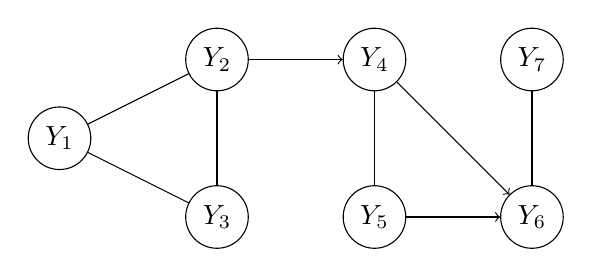
\begin{tikzpicture}
\node[draw,circle] (01) at (-1,-1) {$Y_1$};
\node[draw,circle] (10) at (1,0) {$Y_2$};
\node[draw,circle] (12) at (1,-2) {$Y_3$};
\node[draw,circle] (20) at (3,0) {$Y_4$};
\node[draw,circle] (22) at (3,-2) {$Y_5$};
\node[draw,circle] (32) at (5,-2) {$Y_6$};
\node[draw,circle] (30) at (5,0) {$Y_7$};
\draw[-] (01) -- (10);
\draw[-] (01) -- (12);
\draw[-] (10) -- (12);
\draw[->] (10) -- (20);
\draw[-] (20) -- (22);
\draw[->] (20) -- (32);
\draw[->]  (22) -- (32);
\draw[-]  (32) -- (30);
\end{tikzpicture}
\end{center}
\caption{Example of a probabilistic chain graph model. \label{fig:CG}}
\end{figure}

\gls{PCG} models are an hybrid representation of undirected and directed graphical models, allowing for the underlying graph $\Gr$ to be mixed and more specifically to be a \gls{CG}. We only give here a brief introduction to this class of models \citep[see e.g][for more details]{Cowell1999a, Frydenberg1990, Drton2009, Lauritzen1996a}. Similarly to the other models, we first introduce the relative Markov property, then derive the associated factorization and in conclusion define the model. We let $Bd_i$ be the set of the indices of the variables in the boundary of $Y_i$, $i\in[n]$.

\begin{figure}
\begin{center}
\begin{tikzpicture}
\node[draw,ellipse, minimum height=1cm, minimum width=2cm,inner sep=0pt] (00) at (0,0) {$Y_1, Y_2,Y_3$};
\node[draw,ellipse, minimum height=1cm, minimum width=2cm,inner sep=0pt] (10) at (3,0) {$Y_4, Y_5$};
\node[draw,ellipse,minimum height=1cm, minimum width=2cm,inner sep=0pt](20) at (6,0) {$Y_6, Y_7$};
\draw[->] (00) -- (10);
\draw[->] (10) -- (20);
\end{tikzpicture}
\end{center}
\caption{Representation of the chain graph in Figure \ref{fig:CG} as a directed acyclic graph. \label{fig:CGDAG}}
\end{figure}

\begin{definition}
A probability density $f$ over $\bm{Y}$ is said to obey the chain Markov property relative to a \gls{CG} $\Gr$ with vertex set $\{Y_i:i\in [n]\}$ if for every vertex $Y_i$, $i\in[n]$,
$
Y_i\independent \bm{Y}_{A_i'\setminus Bd_i}\;|\; \bm{Y}_{Bd_i}$.
\end{definition}


\begin{proposition}
If a density $f$ obeys the chain Markov property relative to a \gls{CG} $\Gr$ with vertex set $\{Y_i:i\in[n]\}$, then its density factorizes as
\begin{equation*}
\label{eq:chainfactorization}
f(\bm{y}\;|\; \bm{\theta})= \prod_{i\in[m]} f\left(\bm{y}_{C_i}\;|\; \bm{y}_{\Pi_{C_i}}, \bm{\theta}_{C_i}\right),
\end{equation*}
where $C_1,\dots,C_m$ are the sets of the indices of the variables in the strong components of $\Gr$ and $\Pi_{C_i}=\cup_{j\in C_i}\Pi_j$. 
\end{proposition}


We are now ready to formally define the model.
\begin{definition}
A \gls{PCG} model consists of a \gls{CG} $\Gr$ together with a density $f$ respecting the chain Markov property. 
\end{definition} 

\begin{example}
Consider the \gls{PCG} in Figure \ref{fig:CG}. It can be deduced from this graph that the following conditional independence statements need to hold for a chain Markov distribution
\begin{equation*}
\begin{array}{ll}
Y_4\independent Y_1,Y_3\;|\; Y_2,Y_5,& \ci{Y_5}{Y_1,Y_2,Y_3}{Y_4}, \\
 Y_6\independent Y_1,Y_2,Y_3\;|\; Y_4,Y_5,Y_7,& \ci{Y_7}{Y_1,\dots,Y_5}{Y_6}.
\end{array}
\label{eq:examplechainindependence}
\end{equation*}
Thus for this \gls{PCG} the associated density can be written as
\begin{equation*}
\label{eq:chainexamplefactorization}
f(\bm{y}\;|\; \bm{\theta})=f(y_6,y_7\;|\; y_4,y_5, \bm{\theta}_{67})f(y_4,y_5\;|\; y_3, \bm{\theta}_{34})f(y_1,y_2,y_3\;|\;\bm{\theta}_{123}).
\end{equation*}
\end{example}

Note that each \gls{PCG} can be represented by a less expressive \gls{DAG} whose vertex set corresponds to the strong components of the underlying \gls{CG}. So for example the \gls{PCG} in Figure \ref{fig:CG} can be transformed into the \gls{DAG} of Figure \ref{fig:CGDAG}.
 
\subsubsection{Staged and Event Trees.}
\label{sec:tree}
All the classes of models defined so far are able only to depict standard conditional independence statements. The class of \textit{event tree} models we discuss in this section is able to explicitly represent context specific independences.  Event trees are such that their nodes are the situations in which the process might find itself and the edges emanating from a node are the possible unfoldings given the current situation. It has been extensively discussed in the literature that these models are extremely expressive in describing how processes might unfold especially in the cases where the variables are ordered in a way that follows the narrative of the events \citep{Shafer1996, Freeman2011, Smith2010}. However these can be redundant in the sense that subtrees may be isomorphic, i.e. representing the same unfoldings of situations.
 
In order to define these models, let $\mathcal{T}$ be a directed tree and denote with $\Lambda(v,\mathcal{T})$ the set of paths from $v\in V(\mathcal{T})$ to a leaf node of $\mathcal{T}$. Let $\mathcal{Y}=\Lambda(s_0,\mathcal{T})$, where $s_0$ is the root of the tree, be the set of root-to-leaf paths. Each path $y\in\mathcal{Y}$ is a so-called atomic event, that is a possible unfolding of events. Further let $\mathcal{Y}_s$ denote the set of children of a situation $s\in S(\mathcal{T})$. 

\begin{definition}
An event tree is a directed tree $\mathcal{T}$ together with a random variable $Y_s$ for each situation $s\in S(\mathcal{T})$ with sample space $\mathcal{Y}_s$ defined conditional on having reached vertex $s$. The distribution of $Y_s$ is determined by the \textit{primitive probabilities} $\{\theta_{ss'}=\mathbb{P}(Y_s=s'): s'\in\mathcal{Y}_s\}$. We call $\bm{\theta}_s^\T=(\theta_{ss'})_{s'\in\mathcal{Y}_s}$ the floret probability vector.
\end{definition}

\begin{figure}
\centerline{
\hspace*{-16mm} \xymatrixrowsep{0.5pc}{\xymatrixcolsep{2pc}
\xymatrix{
&&&&\bullet~v_{7}\\
&&&\bullet~v_{3}\ar@[Gruen1][r]_{\text{no}}\ar@[Gruen0][ru]^{\text{yes}}&\bullet~v_{8}\\
&&\bullet~v_{1}\ar[r]_{\text{low}}\ar[ru]^{\text{high}}&\bullet~v_{4}\ar@[Gruen0][r]|{\text{yes}}\ar@[Gruen1][rd]_{\text{no}}&\bullet~v_{9}\\
v_0\hspace*{-16mm}&\bullet\ar[ru]^{\text{yes}}\ar[rd]_{\text{no}}&&&\bullet~v_{10}\\
&&\bullet~v_{2}\ar[r]^{\text{high}}\ar[rd]_{\text{low}}&\bullet~v_{5}\\
&&&\bullet~v_{6}
}}}
\caption{Example of an event tree on three variables with the additional representation of stages in different colors. \label{fig:ET}}
\end{figure}

The expressive power of event trees can be increased by identifying probabilities associated to different edges that are equal. An event tree can be embellished by a colouring of its edges, where two edges have the same colour if their associated probabilities are equal.

\begin{definition}
A \emph{staged tree} is an event tree where for some $s
,s'\in S(\mathcal{T})$, the floret probability vectors are uniquely identified \citep[without permuting their meaning,][]{Cowell2014} and equally coloured. If thus $\bm{\theta}_s=\bm{\theta}_{s'}$ then $s$ and $s'$ are in the same stage. We let $\mathbb{W}$ be the set of stages of $\mathcal{T}$.
\end{definition}
  

\begin{example}
\label{ex:staged}
Suppose a problem is modelled with three binary random variables: $Y_1$, release from a source term; $Y_2$, level of contamination in the surrounding area; $Y_3$, political disruption in the region. Suppose that, once is known whether or not there has been a release from the source term,  the level of contamination does not provide any information to predict the political disruption: i.e. $Y_2\independent Y_3\;|\; Y_1$. This problem can be modelled with a \gls{BN} with vertex set $\{Y_1,Y_2,Y_3\}$ and edge set $\{(Y_1,Y_2), (Y_1,Y_3)\}$. 

However it is believed that when there is no release from the source term, the probability of political disruption is equal to zero. The \gls{BN} model above is not able to represent such an additional information in its graphical representation. This is on the other hand explicitly modelled in the staged tree in Figure \ref{fig:ET}. In this tree the leftmost two edges are the possible outcomes of $Y_1$, the edges in the center the outcomes of $Y_2$ given the different levels of $Y_1$, whilst the rightmost edges coincide with the outcomes of $Y_3$ given $Y_2$ and $Y_1$. In the lower part of the tree, associated to $Y_1=0$, there are no outcomes for the political disruption variable, as these have probability zero. The set of situations of this tree includes vertices $\{v_0,\dots, v_6\}$ and leaves $\{v_{7},\dots, v_{10}\}$. Its stages are $w_0=\{v_0\}$, $w_1=\{v_1\}$, $w_2=\{v_2\}$, $w_3=\{v_3,v_4\}$. Furthermore $\mathbb{W}=\{w_0,\dots,w_3\}$. The tree representation of the associated \gls{BN} model is in Figure \ref{fig:ETBN}. Such a tree is extremely regular in its colouring and each of its root to leaf paths has the same length: a property exhibited by the tree representation of any \gls{BN} (see for more details Section \ref{sec:diff}).
\end{example}

\begin{figure}
\centerline{
\hspace*{-16mm} \xymatrixrowsep{0.5pc}{\xymatrixcolsep{2pc}
  \xymatrix{
&&&&\bullet~v_{7}\\
&&&\bullet~v_{3}\ar@[Gruen1][r]_{\text{no}}\ar@[Gruen0][ru]^{\text{yes}}&\bullet~v_{8}\\
&&\bullet~v_{1}\ar[r]_{\text{low}}\ar[ru]^{\text{high}}&\bullet~v_{4}\ar@[Gruen0][r]|{\text{yes}}\ar@[Gruen1][rd]_{\text{no}}&\bullet~v_{9}\\
v_0\hspace*{-16mm}&\bullet\ar[ru]^{\text{yes~}}\ar[rdd]_{\text{no}}&&&\bullet~v_{10}\\%
&&&&\bullet~v_{11}\\
&&\bullet~v_{2}\ar[rd]_{\text{low}}\ar[r]^{\text{high}}&\bullet~v_{5}\ar@[Gruen1][r]_{\text{no}}\ar@[Gruen0][ru]^{\text{yes}}&\bullet~v_{12}\\
&&&\bullet~v_{6}\ar@[Gruen0][r]|{\text{yes}}\ar@[Gruen1][rd]_{\text{no}}&\bullet~v_{13}\\
&&&&\bullet~v_{14}\\
}}}
\caption{Tree representation of the Bayesian network of Example \ref{ex:staged} .\label{fig:ETBN}}
\end{figure}

Although the colouring of the edges allows for an improved representation of the overall structure of the problem at hand, conditional independences are still difficult to read from the graph. In addition as the number of variables increases, the size of the tree becomes quickly too large to be concisely reported. The class of models we introduce in the following section are able to compactly represent every conditional independence entertained.

\subsubsection{Chain Event Graphs.}
\label{sec:CEG}

\glspl{CEG} \citep{Smith2008} are models capable of representing context specific conditional independences in a single compact graphical representation. \glspl{CEG} are constructed by starting with a staged tree, therefore requiring variables to be discrete, and then by merging into a single vertex certain situations that are in the same stage. 

\begin{definition}
We say that two situations $s$ and $s'$ are in the same \emph{position} if the subtrees with roots $s$ and ${s'}$, respectively, have the same topology and the same edge colouring. We let $\mathbb{B}$ denote the set of positions of a staged tree.
\end{definition}

Note that two situations in the same position are by definition also in the same stage, whilst it does not necessary follows that two situations in the same stage are also in the same position. 

\begin{example}
 Considering the staged tree in Figure \ref{fig:ET}, we can see that for this example the set of stages coincides with the one of positions. 
\end{example} 
 
 \begin{definition}
 A \gls{CEG} is the graph obtained by collapsing a staged tree into its positions. Its vertex set is equal to $\{\mathbb{B}\cup b_{\infty}\}$, where $b_{\infty}$ is the vertex collecting all the leaves of the tree. Its vertex set is such that 
 \begin{itemize}
 \item there is an edge $(b_i,b_j)$, $b_i,b_j\in\mathbb{B}$ for every edge from a generic vertex $v\in b_i$ to any vertex $v'\in b_j$;
 \item there is an undirected edge between any two positions in the same stage;
 \end{itemize}
 \end{definition} 
 
\begin{example}
 The \gls{CEG} representation of the staged tree of Figure \ref{fig:ET} is shown in Figure \ref{fig:CEG}, where we further annotated and coloured the edges as in \citet{Barclay2013a}. 
 \end{example}
 
\begin{figure}
\begin{center}
\begin{tikzpicture}
\node (00) at (0,0) {$b_0$};
\node (1-1) at (2,-1) {$b_2$};
\node (11) at  (2,1) {$b_1$};
\node (21) at (4,1) {$b_3$};
\node (30) at (6,0) {$b_{\infty}$};
\draw[->,sloped, anchor=center, above] (00) to  node {\tiny{yes}} (11);
\draw[->,sloped, anchor=center, above] (00) to  node {\tiny{no}} (1-1);
\draw[->,sloped, anchor=center, above,near start] ([yshift=0.08cm]11.east) to  node {\textcolor{black}{\tiny{high}}} ([yshift=0.08cm]21.west);
\draw[->,sloped, anchor=center, below,near start] ([yshift=-0.08cm]11.east) to  node {\textcolor{black}{\tiny{low}}} ([yshift=-0.08cm]21.west);
\draw[->,Gruen0,sloped, anchor=center, above,near start] ([yshift=0.08cm]21.east) to  node {\textcolor{black}{\tiny{yes}}} ([yshift=0.08cm]30.west);
\draw[->,Gruen1,sloped, anchor=center, below,near start] ([yshift=-0.08cm]21.east) to  node {\textcolor{black}{\tiny{no}}} ([yshift=-0.08cm]30.west);
\draw[->,sloped, anchor=center, above,near start] ([yshift=0.08cm]1-1.east) to  node {\textcolor{black}{\tiny{yes}}} ([yshift=0.08cm]30.west);
\draw[->,sloped, anchor=center, below,near start] ([yshift=-0.08cm]1-1.east) to  node {\textcolor{black}{\tiny{no}}} ([yshift=-0.08cm]30.west);
\end{tikzpicture}
\end{center}
\caption{A chain event graph model representing the staged tree in Figure \ref{fig:ET}. \label{fig:CEG}}
\end{figure}

We chose the \gls{CEG} as a representative model for context specific independences for two main reasons:
\begin{itemize}
\item first, compared to other models capable of  representing context specific conditional independences,  the \gls{CEG} consists of a single graph. Furthermore   \citet{Smith2008} showed that every discrete \gls{BN} can be represented as a \gls{CEG}, whilst the converse does not hold. This is not case for example for probabilistic decision graphs \citep{Jaeger2004} and context specific \glspl{BN} \citep{Boutilier1996}. \citet{Barclay2013a} nicely discusses how to convert a \gls{BN} into a \gls{CEG} model and how to measure the advantages of the latter representation;
\item second, a wide range of methods to perform various statistical analyses have been developed for this model class \citep[see e.g.][]{Barclay2013a,Barclay2014, Freeman2011, Thwaites2010, Thwaites2015}.
\end{itemize}

Importantly, under assumptions similar to local and global independence, but customized for staged trees and \glspl{CEG}, Bayesian updating can be performed in a distributed way through the Multinomial-Dirichlet recursions illustrated in Appendix \ref{sec:multidir}. Let $\mathbb{W}=\{w_i: i\in [n]\}$ be the set of stages of a staged tree where $w_i$ has $n_i$ emanating edges with associated probability vector $\bm{\theta}_i^\T=(\theta_{ij})_{j\in[n_i]}$, such that $\theta_{ij}\in[0,1]$ and $\sum_{j\in[n_i]}\theta_{ij}=1$, $j\in[n_i]$, $i\in[n]$. For a random sample $\bm{x}^\T=(\bm{x}_i^\T)_{i\in[n]}$, where $\bm{x}_i^\T=(x_{ij})_{j\in[n_i]}$ is the vector of the number of units that starts at stage $w_i$ and go through the emanating edges, then it holds
\begin{equation}
\label{eq:liktree}
f(\bm{x}\;|\;\bm{\theta})\propto\prod_{i\in[n]}\prod_{j\in[n_i]}\theta_{ij}^{x_{ij}},
\end{equation}
where we further assumed that $\bm{x}_i\independent \bm{x}_j\;|\;\bm{\theta}$, $i,j\in[n]$, and $\bm{\theta}^\T=(\bm{\theta}_i^\T)_{i\in[n]}$. Therefore the likelihood is multinomial. Now assuming $\bm{\theta}$ has mutually independent parameters, the independence  is retained a posteriori when the prior distribution is updated with the likelihood in equation (\ref{eq:liktree}). In particular this is conjugate if each stage probability vector $\bm{\theta}_i$ is given a Dirichlet prior distribution with parameter $\bm{a}_i^\T=(a_{ij})_{j\in[n_i]}\in\mathbb{R}^{n_i}_{>0}$. The posterior is then again Dirichlet with parameter $\bm{a}_i+\bm{x}_i$. Note that \citet{Freeman2011} proved that assuming mutual independence of the parameters and some other fairly mild conditions, the prior distribution is necessarily Dirichlet.

\subsubsection{Bayes Linear Graphical Models.}
\label{sec:lineargraphs}
We have reviewed a large variety of graphical models to represent various types of factorizations and conditional independences in a full Bayesian setting. Similar methods have been developed within the Bayes linear framework which, instead of using conditional independence, exploits the properties of Bayes linear sufficiency.  We now define the Bayes linear version of a \gls{BN}.

\begin{definition}
 A directed Bayes linear graphical model over $\bm{Y}$ consists of the \gls{DAG} $\mathcal{G}$ with vertex set $\{Y_i: i\in[n]\}$ together with a set of $n-1$ Bayes linear sufficiency statement of the form $\bci{Y_i}{\bm{Y}_{A_i'}}{\bm{Y}_{\Pi_i}}$, for $i\in[n]_1$.
\end{definition}

Mirroring the full Bayesian case, we assume that in a graphical framework is more natural to provide conditional beliefs of a vertex given its parents. Therefore assume that for every vertex $Y_i$ of $\Gr$ the beliefs $\E_{\bm{Y}_{\Pi_i}}^l(Y_i)$ and $\V_{\bm{Y}_{\Pi_i}}^l(Y_i)$ are elicited, $i\in[n]$. Then from Proposition \ref{prop:linearrules} we can deduce that
\begin{equation}
\label{eq:BLDAG1}
\E(Y_i)=\E\left(\E_{\bm{Y}_{\Pi_i}}^l(Y_i)\right),\;\;\;\;\;\;\;\;\V(Y_i)=\V_{\bm{Y}_{\Pi_i}}^l(Y_i)+\V\left(\E_{\bm{Y}_{\Pi_i}}^l(Y_i)\right),
\end{equation}
\begin{equation}
\label{eq:BLDAG2}
\Cov\left(Y_i,\bm{Y}_{\Pi_i}\right)=\Cov\left(\bm{Y}_{\Pi_i},\E_{\bm{Y}_{\Pi_i}}^l(Y_i)\right).
\end{equation}
Therefore given the conditional specification associated to any vertex,  the first two marginal moments and the covariance between any two neighbour vertices can be computed. However the covariance between any two vertices can then be obtained by simply applying equation (\ref{eq:covlin}). Specifically, given that $\bci{Y_i}{\bm{Y}_{[i-1]\setminus \Pi_i}}{\bm{Y}_{\Pi_i}}$ we can deduce that
\begin{equation}
\label{eq:covBNDAG}
\Cov\left(Y_i,\bm{Y}_{\{[i-1]\setminus \Pi_i\}}\right)=\Cov\left(Y_i,\bm{Y}_{\Pi_i}\right)\V\left(\bm{Y}_{\Pi_i}\right)^{+}\Cov\left(\bm{Y}_{\Pi_i},\bm{Y}_{\{[i-1]\setminus \Pi_i\}}\right).
\end{equation} 
By a sequential application of equation (\ref{eq:covBNDAG}) together with (\ref{eq:BLDAG1}) and (\ref{eq:BLDAG2}) through the vertices of the \gls{DAG}, the covariance between any two vertices can therefore be computed. Thus, a full Bayes linear definition of a Bayes linear directed graphical model can be obtained by only eliciting the first two conditional moments associated to every vertex. 
\subsection{Dynamic Models}
\label{sec:dynmod}
In this section we deal with models that allow for a recursive update of the involved probabilities in a dynamic fashion. In the introduction we discussed that Bayesian theory provides a natural framework for forecasting and we now show the basic features of this methodology. For this purpose let $\{\bm{Y}_t\}_{t\in[T]}=\{Y_1(t),\dots, Y_n(t)\}_{t\in[T]}$ be a $n$-dimensional time series with finite time horizon $T$, where $\{Y_i(t)\}_{t\in[T]}$, $i\in[n]$, is a univariate time series, that is the same variable $Y_i$ is measured at various points in time. We let $\mathcal{Y}_i$ and $\bm{\mathcal{Y}}=\bigtimes_{i\in[n]}\mathcal{Y}_i$ be the sample spaces of respectively $Y_i(t)$ and $\bm{Y}(t)$, for any $t\in[T]$. The density function of a generic $Y_i(t)$ is parametrized by  $\bm{\theta}_i(t)\in\bm{\Theta}_i$. Let $I(t)$ be the information known before time $t+1$, $\bm{Y}_A(t)^\T=(Y_i(t))_{i\in A}$, $\bm{Y}_A^t=(\bm{Y}_A(1)^\T,\dots,\bm{Y}_A(t) )^\T$ and $\bm{Y}_{[n]}(t)=\bm{Y}(t)$, for $A\subseteq[n]$. We denote with lower case letters instantiations of these random variables and vectors, and for any $t\in[T-1]$ the sample space of $(\bm{Y}(t),\bm{Y}(t+1))$ is $\bm{\mathcal{Y}}\bigtimes \bm{\mathcal{Y}}$. Similarly to the non-dynamic case, we now introduce a variety of models for time series. 

\subsubsection{Dynamic Linear Models.}
\label{sec:DLM}
The theory of \glspl{DLM} was introduced and formalized by the seminal work of \citet{Harrison1997}. The key property of such class of models is the underlying conditional independence structure which assumes that at each time point all the relevant evidence both observed and collected through time, denote as  $I^{t-1}$, is summarized by the distribution $\bm{\theta}(t)\;|\;I^{t-1}$, where $\bm{\theta}(t)^\T=(\bm{\theta}_i(t)^\T)_{i\in[n]}$ has dimension $r$, and that all the relevant information to predict $\bm{Y}(t)$ is synthesized in $\bm{\theta}(t)$. This is summarized in Figure \ref{fig:CIDLM} implying, for each $t\in [T-1]_1$, $
\ci{\bm{Y}(t)}{I^{t-1}}{\bm{\theta}(t)},$ and  $\ci{\bm{\theta}(t)}{I^{t-1}}{\bm{\theta}(t-1)}$.
 
\begin{figure}
\centerline{
\xymatrix{
&\bm{Y}(t-1)&\bm{Y}(t)&\bm{Y}(t+1)&\\
\ar[r]&\bm{\theta}(t-1)\ar[u]\ar[r]&\bm{\theta}(t)\ar[r]\ar[u]&\bm{\theta}(t+1)\ar[u]\ar[r]&
}}
\caption{Conditional independence structure underlying the dynamic linear model class. \label{fig:CIDLM}}
\end{figure} 

We now introduce the general form of the normal \gls{DLM}. 

\begin{definition}
\label{def:DLM}
The general normal \gls{DLM} is defined by the following three equations.
\begin{align}
&\bm{Y}(t)=F(t)^{\T}\bm{\theta}(t)+\bm{v}(t),  &\bm{v}(t)&\sim N\left(\bm{0},V(t)\right),\label{eq:obseq}\\
&\bm{\theta}(t)=G(t)\bm{\theta}(t-1)+\bm{w}(t),  &\bm{w}(t)&\sim N\left(\bm{0},W(t)\right),\label{eq:evoeq}
\\
&\bm{\theta}(1)\;|\;I^0\sim N\left(\bm{m}(0),C(0)\right),\nonumber \label{eq:ininfo}
\end{align}
where $F(t)$, $G(t)$, $V(t)$, $W(t)$ and $C(0)$ are known matrices of dimensions $r\times n$, $r\times r$, $n\times n$, $r\times r$ and $r\times r$, respectively, with $V(t)$, $W(t)$ and $C(0)$ symmetric, positive semi-definite matrices with positive elements on the diagonal. The vectors $\bm{v}(t)$, $\bm{w}(t)$ and $\bm{m}(0)$ have dimension $n$, $r$ and $n$ respectively.  
\end{definition}
Equation (\ref{eq:obseq}) is the \textit{observation equation} specifying the distribution of $\bm{Y}(t)$ conditional on the \textit{system vector} $\bm{\theta}(t)$, having mean $F(t)^{\T}\bm{\theta}(t)$ and variance $V(t)$, also called \textit{observational variance matrix}. The matrix $F(t)$ is referred to as the \textit{regression matrix}, whilst $\bm{v}(t)$ is the \textit{observational error}. Equation (\ref{eq:obseq}) is the \textit{system evolution equation}, which specifies how the values of the parameter vector evolve trough time. The matrices $G(t)$ and $W(t)$ are called respectively \textit{system transfer} and \textit{system variance} matrices. The vector $\bm{w}(t)$ is called \textit{system error}. 

Note that alternatively the general normal \gls{DLM} can be defined by substituting equations (\ref{eq:obseq})-(\ref{eq:evoeq}) with the following two distributions:
\begin{equation*}
\label{eq:dlmdefinition}
\bm{Y}(t)\;|\;\bm{\theta}(t)\sim N\left(F(t)^{\T}\bm{\theta}(t), V(t)\right),\;\;\;\;\;\;\;\; \bm{\theta}_t\;|\; I^{t-1} \sim N\left(G(t)\bm{\theta}(t-1),W(t)\right).
\end{equation*}

\begin{example}
Special cases of the general normal \gls{DLM} model are:
\begin{itemize}
\item a \textit{univariate \gls{DLM}} is such that $\bm{Y}(t)$ has dimension $1$ (it is therefore a scalar);
\item a \textit{linear univariate \gls{DLM}} is such that $F(t)^\T=(1,X_{1}(t),\dots,X_{r-1}(t))^\T$, where $X_{i}(t)$ is a regressor variable, $i\in [r-1]$;
\item a univariate \textit{regression} \gls{DLM} is such that the entries of $F(t)$ are generic functions of $X_{1}(t),\dots,X_{r-1}(t)$. 
\end{itemize}
\end{example}

Although we do not focus in this thesis on modelling issues, we note here that the theory of \glspl{DLM} comprises a large variety of methodologies to model for example both seasonal and polynomial temporal trends. The concept of \textit{discount factors} is also widely used to elicit the values of the observational variance errors. Importantly, the conditional independence structure underlying \glspl{DLM} provides a natural framework to \textit{intervene} on the system by for example changing the value of some of the model's parameters. This strategy is usually implemented when the model has a poor forecasting performance. We discuss below the role of intervention in causal reasoning. 

The assumption of normality in Definition \ref{def:DLM} is not strictly necessary but it entails some computational advantages. Under this assumption the updating equations of the parameters and the observables can be written in closed form and follow a normal distribution, both in the univariate and the general case. The same property holds for the forecasting distributions, describing the behaviour of the system $k$-steps ahead in the future, for some $k\in\mathbb{Z}_{\geq 1}$.

In practical applications the elicitation of the observational variance is critical and often prohibitive. However, there might be some information regarding its behaviour. Thus in practice $V(t)$ is often assumed unknown and a prior distribution is elicited. In the univariate case, an inverse Gamma distribution can be given to this error, entailing a conjugate analysis as shown in Appendix \ref{sec:nig}. It is then possible to obtain closed recurrences for both the updating and the forecasting distributions which, unconditionally on V(t), follow a T-distribution (see again Appendix \ref{sec:nig}). Although we have shown in Appendix \ref{sec:niw} a conjugate analysis for the multivariate normal model, this does not extend straightforwardly in a dynamic setting as in the univariate case to allow for sequential conjugate learning. We note here though that a variety of methods have been developed to approximate both numerically and analytically these recurrences \citep[see][]{Harrison1997}. Most importantly in the following section we introduce a class of multivariate \glspl{DLM} that entertains exact closed form updating and forecasting routines. 
  
\subsubsection{Multiregression Dynamic Models.}
\citet{Queen1993} introduced the class of \glspl{MDM}, multivariate \glspl{DLM} exhibiting a conditional independence structure between the component time series which remains constant through time. Although each variable is modelled through a simple univariate regression \gls{DLM}, where the regressors are specified by the conditional independence structure, the model class of \glspl{MDM} is in general non Gaussian. The qualitative structure underlying an \gls{MDM} can be represented through a \gls{DAG} whose vertices are the component time series. Importantly, the well known \gls{BN} model we reviewed in Section \ref{sec:BN} is a special case of the \gls{MDM}.

\begin{definition}
\label{def:MDM}
An \gls{MDM} for the time series $\{\bm{Y}(t)\}_{t\in[T]}$ is defined by a \gls{DAG} $\Gr$ with vertex set $\{Y^T_1,\dots,Y^T_n\}$ together with the following $n$ observation equations, system equation and initial information:
\begin{equation*}
\begin{array}{llc}
Y_i(t)=\bm{F}_i(t)^\T\bm{\theta}_i(t)+v_i(t),&v_i(t)\sim (0,V_i(t)),&i\in[n];\\
\bm{\theta}(t)=G(t)\bm{\theta}(t-1)+\bm{w}(t)&\bm{w}(t)\sim(0,W(t));&\\
\bm{\theta}(0)\;|\; I^0\sim (\bm{m}(0),C(0)).
\end{array}
\end{equation*}

The vector $\bm{\theta}_i(t)$ is the system vector, assumed to have dimension $r_i$.  The vector $\bm{F}_i(t)$ of dimension $r_i$ is an arbitrary function of $\bm{y}^t_{\Pi_i}$ and $\bm{y}^{t-1}_i$, but  not $\bm{y}^t_{De_i}$ and $y_i(t)$.  The scalar observation variances  $V_1(t),\dots, V_n(t)$ are positive and can be either known or unknown. The $r\times r$ matrices, $r=\sum_{i=1}^n r_i$, $G(t)=\textnormal{blockdiag}(G_1(t),\dots,G_n(t))$,  $W(t)=\textnormal{blockdiag}(W_1(t),\dots,W_n(t))$ and   $C_0=\textnormal{blockdiag}(C_1(0),\dots,C_n(0))$, are assumed known   and such that $G_i(t)$, $W_i(t)$ and $C_i(t)$ are $s_i\times s_i$ square matrices, functions of $\bm{y}^{t-1}_{Fa_i}$, $i\in [n]$.  The matrices $W_i(t)$ and $C_i(t)$ are also symmetric, positive semidefinite with     positive elements on the diagonal. The errors $v_1(t),\dots,v_n(t)$ and $\bm{w}_1(t),\dots,\bm{w}_n(t)$, where $\bm{w}_i(t)\sim(\bm{0},W_i(t))$, are mutually independent of each other and through time. 
\end{definition} 

\begin{example}
Consider a time series $\{\bm{Y}(t)\}_{t\in[T]}=\{Y_1(t),Y_2(t),Y_3(t),Y_4(t)\}_{t\in[T]}$. An \gls{MDM} having the conditional independence structure depicted by the \gls{DAG} in Figure \ref{fig:MDM} would have observation equations in which $\bm{F}_t(1)$ is a function of $\bm{y}^{t-1}(1)$ and, for $i\in[4]_1$, $\bm{F}_t(i)$ is a function of $y^{t}(i-1)$ and $y^{t-1}(i)$. 
\end{example}

\begin{figure}
\centerline{
\entrymodifiers={++[o][F-]}
\xymatrix{
\bm{Y}^T_1\ar[r]&\bm{Y}^T_2\ar[r]&\bm{Y}^T_3\ar[r]&\bm{Y}^T_4
}
}
\caption{A directed acyclic graph associated to the conditional independence structure of a multiregression dynamic model. \label{fig:MDM}}
\end{figure}

We now report from \citet{Queen1993} two key results associated to \glspl{MDM} which are central for future developments of this thesis. For ease of notation we assume the observational variances to be known, but these results straightforwardly generalize to thhe case of unknown observational variances. 

\begin{proposition}
\label{prop:MDM}
For an \gls{MDM} over a time series $\{Y_1(t),\dots,Y_n(t)\}_{t\in[T]}$, it holds that 
$\independent_{i\in[n]}\bm{\theta}_i(t)\;|\; \bm{y}^{t-1}$  and $
\ci{\bm{\theta}_i}{\bm{y}^t_{[n]\setminus Fa_i}}{\bm{y}_{Fa_i}^t}$.
\end{proposition}
The first conditional independence in Proposition \ref{prop:MDM} indicates that the parameters associated to different component time series remain independent of each other through time. The second one guarantees that a parameter $\bm{\theta}_t(i)$, given the past observations of the variables with indices in the family set, is independent of the rest of the observed data. 

Because of these results, we note that the overall updating of the multivariate time series can be performed locally for each of the component time series independently. Each of these follows, conditionally on the series with indices in the parent set, a simple univariate regression \gls{DLM}. Therefore all the technology briefly reviewed in Section \ref{sec:DLM}, as for example intervention and seasonal trends, can be directly transferred into \glspl{MDM}. Furthermore it is apparent how Proposition \ref{prop:MDM} is a generalization of the distributed learning property in \glspl{BN} under the assumption of global independence we formalized in Proposition \ref{prop:ancupd}.

Note that there is no assumption of normality in the definition of the \gls{MDM}. However a \textit{normal \gls{MDM}} can be defined such that the errors $v_t(i)$ and $\bm{w}_t$ follow a Gaussian distribution. In such cases the overall distribution is non Gaussian, but the forecasting and updating distributions can still be computed analytically and in closed form by using the \gls{DLM} machinery. Therefore \glspl{MDM}, although being multivariate \glspl{DLM}, do not need any approximated method. The following proposition formalizes this fundamental observation.

\begin{proposition}
\label{prop:MDM2}
For an \gls{MDM} over a time series $\{Y_1(t),\dots,Y_n(t)\}_{t\in[T]}$, it holds that 
\begin{equation}
\label{eq:mdmeq1}
f(\bm{y}(t),\bm{\theta}(t)\;|\; I^{t-1})=\prod_{i\in[n]}f(y_i(t)\;|\;\bm{y}_{\Pi_i}(t),\bm{\theta}_i(t), I(t{-1}))\pi(\bm{\theta}_i(t)\;|\;I^{t-1}).
\end{equation}
and 
\begin{equation}
 \label{eq:mdmmarg}
 f\left(\bm{y}(t)\;|\;\bm{y}^{t-1}\right)=\prod_{i\in[n]} g_{ti}\left(\bm{y}^t_{Fa_i},\bm{\theta}_i(t)\right),
 \end{equation}
where
\begin{equation}
g_{ti}=\int_{\bm{\Theta}_i}f\left(y_i(t)\;|\;\bm{y}^{t}_{\Pi_i},\bm{y}^{t-1}_i,\bm{\theta}_i(t)\right)\pi\left(\bm{\theta}_i(t)\;|\;\bm{y}^{t-1}_{Fa_i}\right)\textnormal{d} \bm{\theta}_t(i).
\label{eq:mdmeq2}
\end{equation}
\end{proposition}

\begin{example}
For the \gls{MDM} in Figure \ref{fig:MDM}, equation (\ref{eq:mdmeq1}) can be written as, letting $I=I^{t-1}$ for ease of notation,
\begin{equation*}
\label{eq:factorizationMDMexample}
f(\bm{y}(t),\bm{\theta}(t)\;|\; I)=f(y_1(t)\;|\;\bm{\theta}_1(t),I)\prod_{i\in[4]_1}f(y_i(t)\;|\;\bm{\theta}_i(t),y_{i-1}(t),I)\prod_{j\in[4]}\pi(\bm{\theta}_j(t)|I).
\end{equation*}
The terms in equation (\ref{eq:mdmeq2}) appearing in the forecasting distribution of equation (\ref{eq:mdmmarg}) can be written for this example as
\begin{equation*}
g_{t,i}= 
\left\{
\begin{array}{ll}
\!\!\!\!\int_{\bm{\Theta}_i}f\left(y_i(t)\;|\; \bm{y}^{t-1}_i,\bm{\theta}_i(t)\right)\pi\left(\bm{\theta}_i(t)\;|\; \bm{y}^{t-1}_i\right)\dr \bm{\theta}_i(t), & i=1,\\
\!\!\!\!\int_{\bm{\Theta}_i}f\left(y_i(t)\;|\; \bm{y}^{t-1}_i,\bm{y}^t_{i-1},\bm{\theta}_i(t)\right)\pi\left(\bm{\theta}_i(t)\;|\; \bm{y}^{t-1}_i,\bm{y}^{t-1}_{i-1})\dr \bm{\theta}_i(t\right), & i\in[4]_1.
\end{array}
\right.
\label{eq:exampleMDMpredictive}
\end{equation*}
\end{example}

We now introduce a special case of the \gls{MDM} class, the \textit{linear \gls{MDM}} \citep{Queen1993}, which is very simple to work with. 

\begin{definition}
A \gls{LMDM} is an \gls{MDM} where the errors are assumed to be Gaussian and each component time series is modelled as a univariate linear \gls{DLM}.
\end{definition}
In an \gls{LMDM}, at each time point, each $Y_i(t)$ is modelled as a linear regression with the contemporaneous parent variables as regressors. Therefore the \gls{LMDM} is a dynamic extension of the Gaussian \gls{BN} model defined in Proposition \ref{proposition:ciao2}. 

\begin{example}
The observation equations of an \gls{LMDM} respecting the \gls{DAG} in Figure \ref{fig:MDM} (and using an obvious generalization of the notation in equation (\ref{eq:GausBN})) are as follows
\begin{align}
&Y_1(t)=\theta_{01}(t)+v_1(t), &Y_2(t)=\theta_{02}(t)+\theta_{12}(t)Y_1(t)+v_2(t),\nonumber\\
&Y_3(t)=\theta_{03}(t)+\theta_{23}(t)Y_2(t)+v_3(t),&Y_4(t)=\theta_{04}(t)+\theta_{34}(t)Y_3(t)+v_4(t).\nonumber
\end{align}
\end{example}
\citet{Queen1993} and \citet{Queen2008} describe methods to analytically compute the first two moments of $\bm{Y}(t)$ under the assumption of an \gls{LMDM}. These simply consist of a sequential use of the tower properties of the first two moments. Many of the results we present in the following chapters use the same techniques of conditional moments and generalize the results of these papers. 

Because of its independence properties and its flexibility, the \gls{MDM} has now been successfully applied in practice in many diverse domains: traffic flows \citep{Anacleto2013}, biology \citep{Oates2013}, brain connectivity \citep{Costa2013}, brand sales \citep{Queen1994} and finance \citep{Zhao2015}. Furthermore, a wide tool-kit of more advanced modelling techniques has now been implemented within \glspl{MDM} to allow for causal reasoning \citep{Queen2009}, model choice and averaging \citep{Costa2013,Zhao2015} and heteroscedasticity \citep{Anacleto2013}. 

\subsubsection{Dynamic Chain Graphs.}
\label{sec:DCG}
Although the \gls{MDM} allows for great flexibility in modelling multivariate dynamic domains, its underlying \gls{DAG} structure implies the presence of directional associations only and does not allow for any symmetric relationship. To address this issues, \citet{Queen1992} and \citet{Anacleto2013c} developed the \gls{DCG} model, a multivariate \gls{DLM} whose underlying conditional independence structure can be represented by a \gls{CG}. 

For the purposes of this section only, let $\bm{Y}(t)$ be partitioned into $N$ vector time series of dimensions $n_1,\dots,n_N$, $\sum_{i\in[N]}n_i=n$, so that $\bm{Y}(t)^\T=(\bm{Y}_i(t)^\T)_{i\in[N]}$ where $\bm{Y}_i(t)^\T=(Y_{ij}(t))_{j\in[n_i]}$. Let $\bm{Y}_{ij}^t=(Y_{ij}(1),\dots,Y_{ij}(t))^\T$. Suppose the independence structure is such that any two $\bm{Y}_{ij}^T$ and $\bm{Y}_{ik}^T$ are connected by an undirected edge in the underlying \gls{CG}, $j,k\in [n_i]$, $i\in [N]$. 

\begin{definition}
A \gls{DCG} consists of a \gls{CG} $\Gr$, $V(\Gr)=\{Y_{ij}^T:i\in[N],j\in[n_i]\}$, together with the following $N$ observations equations, system equation and initial information:
\begin{equation*}
\begin{array}{lll}
\bm{Y}_i(t)=\bm{F}_i(t)^\T\bm{\theta}_i(t)+v_i(t),&\bm{v}_i(t)\sim(\bm{0},V_i(t)), &i\in [N],\\
\bm{\theta}(t)=G(t)\bm{\theta}(t{-1})+\bm{w}(t), & \bm{w}(t)\sim(\bm{0},W(t)),&\\
\bm{\theta}(1)\;|\;I(0)\sim (\bm{m}(0),C(0)).
\end{array}
\end{equation*}
The vector $\bm{F}_i(t)^\T=\left(\bm{F}_{ij}(t)^\T\right)_{j\in[n_i]}$ includes the subvectors $\bm{F}_{ij}(t)$, $j\in[n_i]$ of dimension $r_{ij}$, known functions of $\bm{y}^{t-1}_i$ and $\bm{y}^t_{\Pi_{ij}}$, where $\Pi_{ij}$ is the set of the indices of the parents of $\bm{Y}_{ij}^T$ in $\Gr$. The system vector $\bm{\theta}(t)^\T=\left(\bm{\theta}_i(t)^\T\right)_{i\in[N]}$ has dimension $r$, where $\bm{\theta}_i(t)$ is the $r_i$-dimensional system vector for $\bm{Y}_i(t)$, with $r_i=\sum_{j\in[n_i]}r_{ij}$ and $r=\sum_{i\in[N]}r_i$. The $n_i\times n_i$ matrix $V_i(t)$ is the observational variance for $\bm{Y}_i(t)$. The $r\times r$ matrices $G(t)=blockdiag(G_1(t),\dots,G_N(t))$, $W(t)=blockdiag(W_1(t),\dots,W_N(t))$ and $C(0)=blockdiag(C_1(0),\dots,C_N(0))$ are assumed known and such that $G_i(t)$, $W_i(t)$ and $C_i(0)$ are $r_i\times r_i$ square matrices, functions of $\bm{y}^{t-1}_{Fa_i}$. The matrices $C_i(0)$ and $W_i(t)$ are also symmetric, positive semidefinite and with positive elements on the diagonal. The errors $\bm{v}_1(t),\dots, \bm{v}_N(t)$ and $\bm{w}_1(t),\dots,\bm{w}_N(t)$, where $\bm{w}_i(t)\sim N(\bm{0},W_i(t))$, are assumed independent of each other and through time. 
\end{definition}

\begin{figure}
\begin{center}
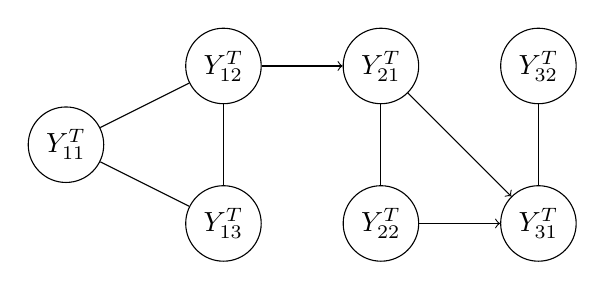
\begin{tikzpicture}[node distance= 2.5cm]
\node[draw,circle] (01) at (-1,-1) {$\bm{Y}_{11}^T$};
\node[draw,circle] (10) at (1,0) {$\bm{Y}_{12}^T$};
\node[draw,circle] (12) at (1,-2) {$\bm{Y}_{13}^T$};
\node[draw,circle] (20) at (3,0) {$\bm{Y}_{21}^T$};
\node[draw,circle] (22) at (3,-2) {$\bm{Y}_{22}^T$};
\node[draw,circle] (32) at (5,-2) {$\bm{Y}_{31}^T$};
\node[draw,circle] (30) at (5,0) {$\bm{Y}_{32}^T$};
\draw[-] (01) -- (10);
\draw[-] (01) -- (12);
\draw[-] (10) -- (12);
\draw[->] (10) -- (20);
\draw[-] (20) -- (22);
\draw[->] (20) -- (32);
\draw[->]  (22) -- (32);
\draw[-]  (32) -- (30);
\end{tikzpicture}
\end{center}
\caption{Dynamic variant of the chain graph model in Figure \ref{fig:CG}. \label{fig:DCG}}
\end{figure}

\begin{example}
Consider the \gls{DCG} defined by the \gls{CG} of Figure \ref{fig:DCG}. Since the topology of this \gls{CG} is the same as the one in Figure \ref{fig:CG}, this \gls{DCG} has three strong components, corresponding, for each time slice $t\in[T]$, to $\bm{Y}_1(t)=(Y_{11}(t),Y_{12}(t),Y_{13}(t))^\T$, $\bm{Y}_{2}(t)=(Y_{21}(t),Y_{22}(t))^\T$ and $\bm{Y}_{3}(t)=(Y_{31}(t),Y_{32}(t))^\T$. Note that in this case we have $\bm{Y}(t)^\T=\left(\bm{Y}_1(t)^\T,\bm{Y}_2(t)^\T,\bm{Y}_3(t)^\T\right)$, as confirmed by Figure \ref{fig:CGDAG}. The observation equations are specified by the following vectors: $\bm{F}_1(t)^\T=\left(\bm{F}_{11}(t)^\T,\bm{F}_{12}(t)^\T,\bm{F}_{13}(t)^\T\right)$, functions of $\bm{y}^{t-1}_1$; $\bm{F}_2(t)^\T=\left(\bm{F}_{21}(t)^\T,\bm{F}_{22}(t)^\T\right)$, functions of $\bm{y}^{t-1}_2$, where $\bm{F}_{21}(t)$ is also a function of $\bm{y}^t_{13}$; $\bm{F}_3(t)^\T=\left(\bm{F}_{31}(t)^\T,\bm{F}_{32}(t)^\T\right)$, function of $\bm{y}^{t-1}_3$, where $\bm{F}_{31}(t)$ is also a function of $\bm{y}^t_2$. 
\end{example}

It can be shown that the results in Propositions \ref{prop:MDM} and \ref{prop:MDM2} for \glspl{MDM} hold for \glspl{DCG} if applied to both the chain component observation series $\bm{Y}_i(t)$ and their associated system vectors $\bm{\theta}_i(t)$, for $i\in [N]$. Therefore in \glspl{DCG} the sequential updating and forecasting of the  relevant probabilities can be distributed across the chain components of the underlying \gls{CG}. We also note that, similarly to \glspl{MDM}, a special linear  model case has been developed for \glspl{DCG} \citep[see][]{Anacleto2013}. 

\subsubsection{Dynamic Bayesian Networks.}
The two above multivariate models are not as commonly used in practice as the \gls{DBN} model class \citep{Murphy2002}. \glspl{DBN} extend the \gls{BN} framework to dynamic and stochastic domains. For the purposes of this thesis, and as often in practice, we consider only \glspl{DBN} respecting the first order Markov assumption: $\ci{\bm{Y}(t)}{\bm{Y}^{t-2}}{\bm{Y}(t-1)}$, for $t\in[T]_2$. We further restrict our attention  to the so-called feed-forward \glspl{DBN}, which assume $\ci{Y_i(t)}{Y_j(t)}{\bm{Y}(t{-1})}$, for any $i,j\in[n]$ and $t\in[T]_1$. These two assumptions imply that there are no edges between variables at the same time point (except for the initial one), and no edges between variables not belonging to adjacent time steps. We also only consider stationary processes. Therefore in this setting the \gls{DBN} model can be simply described by an initial distribution over the first time point and a \gls{BN} having as vertex set two generic time slices, $\bm{Y}(t)$ and $\bm{Y}(t+1)$. Such latter \gls{BN} is usually called \gls{2-TBN}.

\begin{definition}
\label{def:2-TBN}
A \gls{2-TBN} for $\{\bm{Y}(t)\}_{t\in[T]}$ is a \gls{BN} with \gls{DAG} $\Gr$ such that, fixed a $t\in\mathbb{Z}_{\geq 2}$, $t\in [T-1]$, $V(\Gr)=\{Y_i(t),Y_{i}(t+1):i\in[n]\}$, any vertex $Y_i(t)$ has no parents and there are no edges $(Y_{i}(t+1),Y_{j}(t+1))$, $i,j\in[n]$ .   
\end{definition} 
    
\begin{figure}
\centerline{
\entrymodifiers={++[o][F-]}
\xymatrix{
Y_1(t)\ar[d]&Y_2(t)\ar[d]\ar[dl]&Y_3(t)\ar[d]\ar[dl]&Y_4(t)\ar[d]\ar[dl]\\
Y_{1}(t+1)&Y_{2}(t+1)&Y_{3}(t+1)&Y_{4}(t+1)
}
}
\caption{Example of a 2-Time-slice Bayesian network for a multivariate time series comprising four univariate series. \label{fig:2-TBN}}
\end{figure}

\begin{definition}
A \gls{DBN} for the time series $\{\bm{Y}(t)\}_{t\in[T]}$ is a pair $(\Gr,\Gr')$, such that $\Gr$ is a \gls{BN} with vertex set $V(\Gr)=\{Y_i(1):i\in[n]\}$, and $\Gr'$ is a \gls{2-TBN} such that its  vertex set $V(\Gr')$ is equal to $\{Y_i(t),Y_{i}(t+1):i\in[n]\}$.
\end{definition}

It is therefore straightforward to notice that a recursive formula for the density function of a \gls{DBN} similar to the one for \glspl{BN} in Lemma \ref{lemma:rec} exists. This is because a \gls{DBN} can be thought of as the concatenation of \glspl{BN}.

\begin{example}
\label{ex:DBN}
The \gls{BN} in Figure \ref{fig:2-TBN} is a valid \gls{2-TBN} because its topology respects the conditions of Definition \ref{def:2-TBN}. Suppose a \gls{DBN} has such \gls{2-TBN} and the \gls{BN} associated to the initial distribution over $\bm{Y}(1)$ has empty edge set, i.e. represents the independence model in Definition \ref{def:indmodel}. Then its probability density function factorizes as (suppressing the dependence on the parameter vector for ease of notation)
\begin{equation*}
\label{eq:exampleDBNfactorization}
f\left(\bm{y}^T\right)=\prod_{i\in[4]}f(y_i(1))\prod_{t\in[T]_1}f(y_4(t)\;|\;y_{4}(t{-1}))\prod_{j\in[3]}f(y_j(t)\;|\;y_{j}(t{-1}),y_{j+1}(t{-1}))
\end{equation*}
\end{example}

Although \glspl{DBN} entail an effective recursive factorization of the associated density function, thus requiring a low number of probabilities to be elicited in order to fully specify the model, inference in such models cannot be performed as easily as in \glspl{BN}. This is because the initial conditional independence structure is broken through time. As shown in Example \ref{ex:dbn}, after a small number of time steps all the variables in a same time slice become correlated with each other. Independence can only be retained if each component time series is independent of the others, that is if the \gls{2-TBN} has edges of the type $(Y_i(t),Y_i(t+1))$ and an initial distribution described by an independence model. Therefore the efficient and distributed recursions for both inference and forecasting associated to \glspl{MDM} and \glspl{DCG} do not transfer to generic \glspl{DBN}. However we note here that a variety of methodologies based on stochastic approximated methods have been developed to allow for tractable inference in such models \citep{Boyen1998, Koller2001}. 

\begin{example}
\label{ex:dbn}
The \gls{DAG} in Figure \ref{fig:unrolled} \citep[from ][]{Boyen1998} is the so-called unrolled version of the \gls{DBN} of Example \ref{ex:DBN} over the first four time points. It is apparent from this network that at time step $4$ all the processes are correlated with each other.
\end{example}

\begin{figure}
\centerline{
\entrymodifiers={++[o][F-]}
\xymatrix{
Y_1(1)\ar[r]&Y_2(1)\ar[r]&Y_3(1)\ar[r]&Y_4(1)\\
Y_1(2)\ar[r]\ar[ur]&Y_2(2)\ar[r]\ar[ur]&Y_3(2)\ar[r]\ar[ur]&Y_4(2)\\
Y_1(3)\ar[r]\ar[ur]&Y_2(3)\ar[r]\ar[ur]&Y_3(3)\ar[r]\ar[ur]&Y_4(3)\\
Y_1(4)\ar[r]\ar[ur]&Y_2(4)\ar[r]\ar[ur]&Y_3(4)\ar[r]\ar[ur]&Y_4(4)}}
\caption{Unrolled version of the dynamic Bayesian network of Example \ref{ex:DBN} with 2-Time-slice Bayesian network of Figure \ref{fig:2-TBN}.\label{fig:unrolled}}
\end{figure}

\subsection{Causality}
\label{sec:causality}
Statistical reasoning has historically overlooked the inspection of causal relationships between random variables. Standard methods, as for example regression analysis, is in general only able to predict new values of a variables given a set of covariates, and how these relate to the variable under inspection. Until recently, there has not been a formal study of causal relationships between sets of random variables to assess, for example, whether a variable can be considered as a \textit{cause} for another one or not.

 \citet{Pearl2000} and \citet{Spirtes1993}, among the others, provide a systematic study of the causal mechanisms underlying a given \gls{BN} model when certain variables are \textit{manipulated} and fixed to take a certain value in their sample space. This theory supposes the existence of an underlying idle system, that is one where its variables are observed and not manipulated to a certain value. 
 
\citet{Shafer1996} discusses causal reasoning for models depicted by trees. As also suggested by \citet{Smith2010}, trees are particularly suitable to represent causal relationships, since these can uniquely describe the actual narrative underlying the unfolding of events. We also note here that causal reasoning is more tenable for Bayesian decision analysis than in pure inferential reasoning since \glspl{DM} need to think hard on how the problem at hand unfolds when eliciting both their probabilistic and preferential beliefs. Therefore, a \gls{DM}'s model can often be used to answer various causal questions \citep{Smith2010}.

In this section we first formalize what we mean by manipulate (or intervene on) a system and introduce various types of interventions. We then consider \glspl{CBN} and examine the link between global and local independence assumptions and causality. We then conclude by briefly introducing some other causal models. 

\subsubsection{Interventions.}
We now formally define the concept of intervention as introduced in \citet{Pearl2000}.

 \begin{definition}
 A Perlean intervention on $\bm{Y}_A$, $A\subset[n]$, consists of fixing these variables to a (known) value $\bm{y}_A$. The resulting density is written $f\left(\bm{y}\;|\;do(\bm{Y}_A=\bm{y}_A)\right)$.
 \end{definition} 

Perlean interventions therefore work at the random variables level. However, often in practice, as for example during controlled randomized experiments, probabilities are fixed to certain specific values. This is also a common practice within the literature of \glspl{DLM} where it is referred to as \textit{monitoring} \citep{Harrison1997,West1986,West1989}. In the case the prediction performance of a model starts to decrease then the user can intervene in the model and change the value of some of its parameters to more suitable ones.  

\begin{definition}
For $A\subseteq[n]$, a stochastic intervention on a parameter $\bm{\theta}_A$ consists of fixing it to a known new value $\hat{\bm{\theta}}_A$. This intervention is denoted as $do(\bm{\theta}_A=\hat{\bm{\theta}}_A)$.
\end{definition}
 
Such interventions have been studied for example to investigate causal reasoning in \glspl{CEG} \citet{Thwaites2010}. \citet{Daneshkhah2004} defines a special type of stochastic intervention called \textit{contingent randomized intervention} which changes the parameter vector associated to a \gls{BN}. 
 
\subsubsection{Causal Bayesian Networks.}
As noted in Section \ref{sec:BN}, there are several \glspl{BN} entertaining the same density factorization and therefore leading to the same kind of inferences. Causal reasoning cannot thus be straightforwardly followed in generic \glspl{BN}. We define here a particular class of \glspl{BN} that are causal in the Perlean sense.

\begin{definition}
\label{def:cbn}
A \gls{BN} $\Gr$ is a \gls{CBN} if, for any Perlean intervention on $\bm{Y}_A$, $A\subset[n]$, it holds that 
\begin{equation*}
f\left(\bm{y}\;|\;\bm{\theta},do(\bm{Y}_A=\bm{y}_A)\right)=\prod_{i\in[n]\setminus A}f\left(y_i\;|\;\bm{\theta}_i,\bm{y}_{\Pi_i}\right).
\end{equation*} 
\end{definition} 

\begin{example}
Consider the \gls{BN} with \gls{DAG} in Figure \ref{fig:BNexample}. Suppose we intervene on this \gls{DAG} and set $Y_2=y_2$. The resulting factorization is equal to
\begin{equation*}
f\left(y_1,y_2,y_3,y_4\;|\;\bm{\theta},do(Y_2=y_2)\right)=f(y_1\;|\;\bm{\theta}_1)f(y_3\;|\;y_1,y_2,\bm{\theta}_3)f(y_4\;|\;y_1,\bm{\theta}_4).
\end{equation*}
Such intervention can be depicted graphically by deleting every edge into $Y_2$, in this case simply $(Y_1,Y_2)$, and changing the label of the vertex associated to the intervened variable to $Y_2=y_2$. Such \gls{DAG} is reported in Figure \ref{figure:causalBN}.
\end{example}

\begin{figure}
\vspace{0.3cm}
\entrymodifiers={++[o][F-]}
\centerline{
\xymatrix{
\mbox{\large{$Y_4$}}&\mbox{\large{$Y_2=y_2$}}\ar[d]\\
\mbox{\large{$Y_1$}}\ar[u]\ar[r]&\mbox{\large{$Y_3$}}
}
}
\vspace{0.3cm}
\caption{
Causal version of the Bayesian Network in Figure \ref{fig:BNexample} under the intervention $Y_2=y_2$. \label{figure:causalBN}}
\end{figure}

\begin{definition}
For an intervention $do(\bm{Y}_A=\bm{y}_A)$ over the variables of a \gls{BN} $\Gr$, $V(\Gr)=\{Y_1,\dots,Y_n\}$, we call \emph{manipulated \gls{DAG}} $\Gr'$ the network with edge set $\E(\Gr')=\E(\Gr)\setminus\{(Y_i,Y_j)\in E(\Gr): j\in A\}$ and $V(\Gr')=\{Y_i: i\in \{[n]\setminus A\}\}\cup \{Y_i=y_i: i\in A\}$.
\end{definition}

If a \gls{BN} is believed to be causal, then experimental evidence can be used to update the parameter densities as formalized below.

\begin{proposition}
 Suppose global independence holds and assume the experimental sample $\bm{x}$ from the same population as $\bm{Y}$ is ancestral with respect to the manipulated \gls{DAG} for the intervention $do(\bm{Y}_A=\bm{y}_A)$. Let $I$ be the set of indices of the vertices whose children are not sampled. Then for a \gls{CBN} the posterior is equal to
 \begin{equation*}
 \pi(\bm{\theta}\;|\;\bm{x})=\prod_{l\in I}\prod_{\substack{j\in A_l\\j\not\in A}}\pi(\bm{\theta}_j\;|\;\bm{x})\prod_{k\not\in \{A_l\cup A\}}\pi(\bm{\theta}_k).
 \end{equation*}
\end{proposition}

The concept of causality for \glspl{BN} has been extended to take into account manipulation of the parameter vertex in \citet{Daneshkhah2004}, just as the concept of a Markov distribution has been translated at the parameter level into hyper Markov laws. They defined the concept of an hypercausal \gls{BN}, which is one where contingent randomised interventions respect the topology of the \gls{DAG}. Most importantly they showed that local and global independence hold \gls{iff} the \gls{BN} is hypercausal and therefore also in the case the model is \gls{CBN}. Thus the validity of the causal assumption can be checked through reasoning about the faithfulness of global and local independence and vice versa. 

We have focused here on causality over graphical directed structures, since these naturally provides a framework for causal reasoning. In these models variables are ordered and there are not symmetric relationships. This is the reason why causal arguments in \gls{MN} models are much more difficult to develop \citep[see e.g.][]{Lauritzen2002}

\subsubsection{Other Causal Models.}
Although much of the literature on statistical cau-sality centred on the \gls{BN} model class, the causal semantic has been extended to a variety of frameworks, e.g. \glspl{CEG} \citep{Thwaites2010}, \glspl{CG} \citep{Lauritzen2002}, \glspl{DBN} \citep{Eichler2007}, \glspl{ID} \citep{Dawid2002a} (see Section \ref{sec:id}), \glspl{MDM} \citep{Queen2009} and  others \citep{Aalen2012, Dawid2010, Smith2007}. 
 
In this section we focus on \glspl{MDM} in order to give an illustration of  both stochastic intervention and causal reasoning in dynamic environment. It has been shown in \citet{Queen2009} that the \gls{MDM} is able to identify contemporaneous causal relationships: similar results do not hold in general for generic \glspl{DBN} \citep{Eichler2007}.  There are two possible types of stochastic intervention in \glspl{MDM}: one changing the observation equation, the other manipulating the system equation. If an intervention is implemented at time $t$, then this is before observing $\bm{Y}(t)$. An intervention for the observation equation is formalized as
\begin{equation}
\label{eq:intobs}
Y_i(t)\;|\;\bm{Y}_{\Pi_i}(t),I(t{-1}),do\left(\bm{\theta}_i(t)=\hat{\bm{\theta}}_i(t), V_i(t)=\hat{V}_i(t)\right)\sim (\hat{\theta}_i(t),\hat{V}_i(t)),
\end{equation}  
whilst manipulating the system equation entails
\begin{equation}
\label{eq:intsys}
\bm{\theta}_i(t)\;|\;\bm{\theta}_i(t{-1}),I(t{-1}),do\left(\bm{\theta}_{i}(t{-1})=\hat{\bm{\theta}}_i(t{-1}),W_i(t)=\hat{W}_i(t)\right)\sim (\hat{\bm{\theta}}_i(t{-1}),\hat{W}_i(t)).
\end{equation}

Before observing $\bm{Y}(t)$, an intervention of the type in equation (\ref{eq:intobs}) affects the forecast of $Y_i(t)$ and $\bm{Y}_{[n]_{i-1}}(t)$ only, whilst an intervention as in equation (\ref{eq:intsys}) affects the distribution of  $\pi(\bm{\theta}_i(t+s))$, $Y_i(t+s)$ and  $\bm{Y}_{[n]_{i-1}}(t+s)$, $s\in[T{-t}]^0$. The effects of these interventions after the observation of $\bm{Y}_t$ are different, although the interventions are still applied before observing this vector. In particular the two interventions affect the same quantities after observing $\bm{Y}_t$. These change the posterior distribution of $\bm{\theta}_i(t)$ and $\bm{\theta}_{[n]_{i-1}}(t)$ and the forecasts of $\bm{\theta}_i(t+s)$, $\bm{\theta}_{[n]_{i-1}}(t+s)$, $Y_i(t+s)$ and $\bm{Y}_{[n]_{i-1}}(t+s)$ for $s\in[T{-t}]^0$. 

These interventions are used to identify the correct causal structure underlying a dynami process. \citet{Queen2009} considers a multi-process \gls{MDM} which is a mixture of \glspl{MDM} with weights representing the probability of that model being the true causal description of the process. When interventions are implemented, the weight of the true model increases, allowing for the identification of the \gls{DAG} describing the causal relationships between the variables.
 
Before concluding this section, we point out that \citet{Dawid2010} developed causal arguments in the framework of dynamic treatment strategies \citep{Murphy2003}. These are dynamic models in medical contexts where the objective is to identify the causal effect of a particular treatment. The computation of these effects is based on backward inductive arguments, which mirrors the recursions we develop in Chapter \ref{chapter4} for \glspl{IDSS}. 
 
\subsection{Emulators} 
\label{sec:emu}
Although probabilistic reasoning is now widespread in many areas of science, deterministic modelling is still often performed in practice as noted in Chapter \ref{chapter1}. Such deterministic models usually consist of huge simulators using approximated methods to numerically solve big systems of differential equations describing some natural process. This is often the case in climate change modelling for example \citep{Rougier2015}.

For coherent Bayesian analyses using deterministic computer models, there is the need to define a probability distribution over the outputs of such systems. This is because unmodelled uncertainty appears at various stages of the deterministic computations of simulators as extensively discussed in \cite{Kennedy2000}. Probability distributions are then usually achieved by building an \textbf{emulator} over their outputs. The literature on emulators is now very vast \citep{Kennedy2006, Kennedy2001,OHagan2006,Santner2003} and for the purposes of this thesis we focus here only on Bayesian methods. 

Within the Bayesian literature a variety of methodologies have been developed to account for both large-dimensional and dynamic outputs \citep{Conti2009,Liu2009, Rougier2008}. We also note here that emulators working within the Bayes linear framework are now well established and used in practice \citep{Craig2001, Goldstein2006, Williamson2011}.

\subsubsection{Modelling of Computer Outputs.}
A simulator is a function $g(\cdot)$ that maps inputs $\bm{z}\in\bm{\mathcal{Z}}$, for some arbitrary space $\bm{\mathcal{Z}}$, into an output $y=g(\bm{z})$. In its vanilla form the output $y$ is univariate and constant through time. Often in practice only a small set of training runs at inputs $\bm{z}_1,\dots, \bm{z}_N$ of the simulator are available, whose outputs $y_1=g(\bm{z}_1),\dots, y_N=g(\bm{z}_N)$ are observed and treated as data. Only a small number of such outputs can be observed since simulators are usually slow and each single evaluation can take weeks if not months. An emulator is then an approximation $\hat{g}(\cdot)$ of $g(\cdot)$ such than at an input point $\bm{z}_i$, $\hat{g}(\bm{z}_i)=g(\bm{z}_i)$, whilst at other points it consists of a distribution whose mean represents a plausible interpolation of the training runs and its variance the uncertainty associated to such interpolation.

\subsubsection{Gaussian Process Modelling.}
The most common modelling technique is to assume that $g(\cdot)$ behaves as a \textit{\gls{GP}}. Formally, $g(\cdot)$ has a \gls{GP} distribution if, for every $N\in\mathbb{Z}_{\geq 1}$, the joint distribution of $g(\bm{z}_1),\dots,g(\bm{z}_N)$ is multivariate normal for all $\bm{z}_1,\dots,\bm{z}_N\in\bm{\mathcal{Z}}$. The distribution of the \gls{GP} is therefore characterized by its mean $m(\bm{z})=\mathbb{E}(g(\bm{z}))$ and its covariance function $c(\bm{z},\bm{z}')=\Cov(g(\bm{z}),g(\bm{z}'))$, for $\bm{z},\bm{z}'\in\bm{\mathcal{Z}}$. In general, $m(\cdot)$ may be any function, but $c(\cdot,\cdot)$ is non negative definite for every $\bm{z}_1,\dots,\bm{z}_N\in\bm{\mathcal{Z}}$ and any $N\in\mathbb{Z}_{\geq 1}$.

The mean and covariance functions are usually modelled hierarchically as
\begin{equation*}
\label{eq:emulator}
g(\bm{z})=m(\bm{z})+e(\bm{z})=\bm{h}(\bm{z})^\T\bm{\beta}+e(\bm{z}),
\end{equation*}
where $\bm{h}(\bm{z})^\T=(h_i(\bm{z}))_{i\in[p]}$ is a vector of $p$ known functions, $\bm{\beta}^\T=(\beta_i)_{i\in[p]}$ is a vector of $p$ unknown coefficients and $e(\bm{z})$ is a mean-zero \gls{GP}  with covariance $c(\cdot,\cdot)$.
The vector $\bm{h}$ often simply consists of simple monomial functions of $\bm{z}$. The covariance is usually defined as 
\begin{equation*}
\label{eq:emulatorcovariance}
c(\bm{z},\bm{z}')=\sigma^2r(\bm{z}-\bm{z}'),
\end{equation*}
where $r(\cdot)$ is a correlation function such that $r(0)=1$, $\bm{z},\bm{z}'\in\bm{\mathcal{Z}}$. This choice implies a stationary process since the correlation only depends on the distance between two points. A variety of correlation functions have been defined in the literature and these are often used in geostatistical modelling \citep{Diggle2007}. For example the exponential correlation function can be written as
\begin{equation*}
\label{eq:emulatorcorrelation}
r(\bm{z}-\bm{z}')=\exp\left(-\sum_{i\in[q]}\omega_i(z_i-z_i')^2\right),
\end{equation*}
where $q$ is the dimension of $\bm{\mathcal{Z}}$. The model definition is then completed by eliciting a prior distribution over the parameters $\bm{\beta}$, $\sigma^2$ and $\bm{\omega}^\T=(\omega_i)_{i\in[q]}$. Often a weak improper prior is given to such parameters, but conjugate analysis can be performed by choosing appropriate prior distributions similarly to the normal linear model case. 

Once an emulator is built, using for example the \gls{GP} structure we exemplified here, each evaluation of the simulator can be used to update the the probability distribution of the emulator in a Bayesian fashion. Furthermore, additional uncertainty measures can be included in the modelling. For example, calling $\bm{y}_i'$ the true value of the system the simulator is modelling given observed inputs $\bm{z}_i$, one could set $y_i'=f(\bm{z}_i)+v$, where $v$ is some error following for example a Gaussian distribution \citep[see][for more comments on these modelling techniques]{Kennedy2000}.

\section{Utility Models}
\label{sec:ut}
The other main ingredient of the \gls{SEU} model is the utility function $u(\bm{r},d)$. In this section we provide a broad overview of utility theory with particular focus to the multi-attribute case, that is when $\bm{R}$ is large dimensional. For the purposes of this section we let $\bm{R}=(R_1,\dots,R_m)$ and $\bm{r}$ and $r_i$ be instantiations of $\bm{R}$ and $R_i$ respectively. Note that in the notation of Section \ref{sec:SEU}, each $R_i$ can correspond to random quantities, decisions, or a combination of the two. For ease of notation in this section we simply use the symbols $r_i$s.

 Here we first introduce independence concepts for preferences, mirroring those for probabilistic reasoning; we  then show how particular sets of independence assumptions can lead to classes of utility factorizations that, similarly to the probabilistic case, can highly reduce the burden of utility elicitation; we then consider fairly recent utility factorizations that arise from underlying graphical models depicting preferential indifferences; we conclude the section with a review of utility theory for single attributes which, under the assumption of a particular utility factorization, comes often into play in multivariate settings. 

Before that, we briefly summarize here important aspects of utility theory that we do not deal with in this thesis since they are not central for our results. First, although value functions are widely used in practice \citep{Belton2002,Keeney1993a}, these are not introduced in this thesis. There are two main reasons for this: one, the coherence and the rationale of the Bayesian formalism is retained only using utility functions; two, value functions, differently from utilities, are not able to represent attitudes towards risk. 

Furthermore, we  assume in this thesis that the vector $\bm{R}$ includes a \textit{complete} and \textit{non-redundant} collection of attributes so that this covers all the important aspects of the problem and each factor is not double counted. In addition each $R_i$ has to be \textit{operational} so that it can be meaningfully used in the analysis and the \gls{DM} can provide true preferential assessments about it.  More broadly, we assume that the vector $\bm{R}$ includes all the relevant factors of the system under study and the \gls{DM} can uniquely provide preferential assessments over its elements. In practice to identify such set of attributes an \textit{objective tree} \citep{Keeney1993a} is built, which breaks down each attribute into sub-attributes until the leaves of tree consists of operational attributes only. An example of the objective tree elicited during the Chernobyl project is presented in Figure \ref{fig:objtree}. Each leaf of this tree would correspond in our notation to an element $R_i$ of $\bm{R}$.

Finally, we do not discuss techniques to assess and elicit utility functions, meaning their algebraic form and their  features \citep[see e.g.][]{Keeney1993a}.

\begin{figure}
\begin{center}

\begin{tikzpicture}[>=stealth',shorten >=1pt,auto,semithick,
    fact/.style={rectangle, draw=none, rounded corners=1mm, fill=blue, drop shadow,
        text centered, anchor=north, text=white},
        leaf/.style={rectangle, draw=none, fill=red,
        text centered, anchor=north, text=white, drop shadow},
    level distance=0.5cm, growth parent anchor=south
]
\tikzstyle{every state}=[every text node part/.style={align=center}]
\node (State00) [fact] {Humans' living} [->] [sibling distance=4cm]
child{  [sibling distance=5cm]
        node (Fact01) [fact] {Effects}
        child{ [sibling distance=2cm]
        node (Fact11) [fact] {Health}
        child{[sibling distance=3cm]
        node (Fact21) [fact] {Radiation}
        child{ 
        node (Fact31) [leaf] {Hereditary}
        }
        child{
        node (Fact31) [leaf] {Number of  cancers}
        }
        }
        child{
        node (Fact23) [leaf] {Stress}
        }
        }
        child{
        [sibling distance=3cm]
        node (Fact33) [fact] {Acceptability}
        child{
        node (leaf11) [leaf] {Affected  Regions}
        }
        child{
        node (leaf22) [leaf] {Rest of  URSS}
        }
        }
        }
child{
        node (Fact02) [leaf] {Resources}
        }
        ;
\end{tikzpicture}
\end{center}
\caption{Objective tree elicited at the end of the Chernobyl project from \citet{Papamichail2013}. The vertices in red of the tree are leaves, whilst the blue ones are positions. \label{fig:objtree}}
\end{figure}
 
\subsection{Independence Concepts}
As the dimension of $\bm{R}$ might be arbitrarily large, a variety of independence concepts have been introduced in the literature to both simplify the utility elicitation and describe various sets of indifferences. Here we introduce a few of these.

\begin{definition}
\label{def:utind}
An attribute $\bm{R}_A$ is said to be \textbf{\gls{UI}} of $\bm{R}_B$, for a partition $A$, $B$ of $[m]$, if the utility for $\bm{R}_A$ does not change when the attributes in $\bm{R}_B$ are varied.
\end{definition}

\begin{proposition}
Under the conditions of Definition \ref{def:utind}, if $\bm{R}_A$ is \gls{UI} of $\bm{R}_B$ then
\begin{equation*}
\label{eq:utilityindependence}
u(\bm{r})=a(\bm{r}_B)+b(\bm{r}_B)u(\bm{r}_A)
\end{equation*}
where $a(\cdot)$ and $b(\cdot)>0$ depend on $\bm{r}_{B}$ and not on $\bm{r}_A$. 
\end{proposition}

In order to understand the meaning of this independence, consider the following example. If the \gls{DM} believes that the prevalence of tumours is \gls{UI} of the amount of contamination, then the utility function describing the prevalence of tumours does not depend on the level of contamination of the area. For example, the utility of having a low number of cancer cases would be the same both when the area is highly contaminated and when there is no radiation at all. Note that utility independence is not necessarily symmetric: if the prevalence of tumours is \gls{UI} of the level of contamination then it does not follow that the converse is true.

We now consider two particular sets of \gls{UI} statements.

\begin{definition}
We say that $\bm{R}$ has \gls{suia} if  $R_i$ \gls{UI} $\bm{R}_{[m]\setminus \{i\}}$, $i\in[m]$.
\end{definition}

\begin{definition}
We say that $\bm{R}$ has \gls{muia} if, for every $A\subseteq[m]$, $\bm{R}_A$ \gls{UI} $\bm{R}_{[m]\setminus A}$.
\end{definition}

We now consider a generalization of utility independence.
\begin{definition}
\label{def:cutind}
An attribute $\bm{R}_A$ is said to be \textbf{\gls{CUI}} of $\bm{R}_B$ given $\bm{R}_C$, for a partition $A$, $B$, $C$ of $[m]$, if the utility of $\bm{R}_A$ does not change when the attributes in $\bm{R}_B$ are varied, for each instantiation of $\bm{R}_C$.
\end{definition}


\begin{proposition}
Under the conditions of Definition \ref{def:cutind}, if $\bm{R}_A$ is \gls{CUI} of $\bm{R}_B$ given $\bm{R}_C$ then
\begin{equation}
u(\bm{r})=a(\bm{r}_B,\bm{r}_C)+b(\bm{r}_B,\bm{r}_c)h(\bm{r}_A,\bm{r}_C)
\label{eq:cui}
\end{equation}
for some $a$, $h$ and $b>0$ function of their arguments only. 
\end{proposition}

In order to give an explicit form to the function $h$ of equation (\ref{eq:cui}) in terms of utility functions, we introduce a generalization of the utility function of Definition \ref{def:ut}, which more easily can represent \gls{CUI} statements. Let $\bm{r}_A^{*}=(r_i^{*})^\T_{i\in A}$ and $\bm{r}_A^0=(r_i^0)^\T_{i\in A}$, $A\subseteq [n]$, where $r_i^*$ and $r_i^0$ are respectively the bests and the worst outcome of attribute $R_i$. 

\begin{definition}
\label{def:cui}
The normalized conditional utility function for $\bm{R}_A$ given $\bm{R}_{[m]\setminus A}$ is defined as
\begin{equation*}
u(\bm{r}_A\;|\; \bm{r}_{A^c})=\frac{u(\bm{r}_A,\bm{r}_{[m]\setminus A})-u(\bm{r}_A^0,\bm{r}_{[m]\setminus A})}{u(\bm{r}_A^*,\bm{r}_{[m]\setminus A})-u(\bm{r}_A^0,\bm{r}_{[m]\setminus A})}.
\end{equation*}
We also define the normalized conditional disutility function as
\begin{equation*}
\hat{u}(\bm{r}_A\;|\;\bm{r}_{[m]\setminus A})=1-u(\bm{r}_A\;|\;\bm{r}_{[m]\setminus A})
\end{equation*}
\end{definition}

\begin{proposition}
Under the conditions of Definition \ref{def:cutind}, if $\bm{R}_A$ \gls{CUI} $\bm{R}_B$ given $\bm{R}_C$ then
\begin{equation*}
u(\bm{r}_A\;|\; \bm{r}_B,\bm{r}_C)=u(\bm{r}_A\;|\; \bm{r}_B^0,\bm{r}_C)=u(\bm{r}_A\;|\; \bm{r}_B^{*},\bm{r}_C).
\end{equation*}
Furthermore, the terms in equation (\ref{eq:cui}) can be written as 
$
a(\bm{r}_B,\bm{r}_C)=u(\bm{r}_A^0,\bm{r}_B,\bm{r}_C)$, $b(\bm{r}_B,\bm{r}_C)=u(\bm{r}_A^*,\bm{r}_B,\bm{r}_C)-u(\bm{r}_A^0,\bm{r}_B,\bm{r}_C)$ and $h(\bm{r}_B,\bm{r}_C)=u(\bm{r}_C\;|\;\bm{r}_B^0,\bm{r}_C)$.
\end{proposition}

We now introduce a different class of independence concepts. 

\begin{definition}
Let $B_1,\dots,B_k$ be a partition of $[m]$. Attributes $\bm{R}_{B_1},\dots, \bm{R}_{B_k}$ are said  to be additive independent if the preference comparison of any two lotteries, defined as probability distributions over $\bigtimes_{i\in[k]} \bm{R}_{B_i}$, depends only on their marginal probability distributions.
\end{definition}

Additive independence can be generalized to the case when the indices of the attributes do not form a partition of $[m]$. 
\begin{definition}
\label{def:GAI}
Let $B_1,\dots,B_k$ be such that $\cup_{i\in[k]}A_i=[m]$. Attributes $\bm{R}_{B_1},\dots, \bm{R}_{B_k}$ are said to be \gls{GAI} if the the preference comparison of any two lotteries depends only on the marginal probability distributions over $\bigtimes_{i\in[k]} \bm{R}_{B_i}$.
\end{definition}

\subsection{Utility Factorizations}
The sets of independences introduced in the previous section give rise to specific factorizations of the overall utility function. Suppose each function $u_A(\bm{r}_A)$, a marginal utility function over $\bm{R}_A$ only, is such that $u_i(\bm{r}_A^0)=0$ and $u_i(\bm{r}_A^*)=1$, $A\subseteq [m]$. The following results hold.

\begin{proposition}
If a utility function $u(\bm{r})$ has $m$ \gls{suia}, then it must take the form 
\begin{equation}
\label{eq:multilinear}
u(\bm{r})=\sum_{A\in\mathcal{P}_0([m])}k_A\prod_{i\in A} u_i(r_i),
\end{equation}
where $\mathcal{P}_0$ denotes the power set without the empty set and $k_A\in [0,1]$ is a \textit{criterion weight} \citep{Keeney1993a} such that $\sum_{A\subseteq[m]}k_A=1$.
\end{proposition} 

\begin{definition}
\label{def:multilinear}
Utility functions entertaining the factorization in equation (\ref{eq:multilinear}) are called \textbf{multilinear}.
\end{definition}

The criterion weights of equation (\ref{eq:multilinear}) can be evaluated by comparing the utility of terms $u(\bm{r}_A^*,\bm{r}_{[m]\setminus A}^0)$. Their actual form is not fundamental for this thesis and can be found in \citet{Keeney1993a}. 

\begin{proposition}
\label{prop:multiplicative}
If a utility function $u(\bm{r})$ has $m$ \gls{muia}, then it must take the form
\begin{equation}
\label{eq:multiplicative}
u(\bm{r})=\sum_{A\in\mathcal{P}_0([m])}h^{n_A-1}\prod_{i\in A}k_iu_i(r_i),
\end{equation}
where $n_A$ is the number of elements in $A$, $k_i=u\left(r_i^*,\bm{r}_{[n]\setminus \{i\}}^0\right)$ and $h$ is the unique solution not smaller than minus one to
\begin{equation}
\label{eq:h}
1+h=\prod_{i\in[m]}(1+hk_i).
\end{equation}
\end{proposition}

\begin{definition}
\label{def:multiplicative}
Utility functions entertaining the factorization in equations (\ref{eq:multiplicative}) and (\ref{eq:h}) are called \textbf{multiplicative}.
\end{definition}

\begin{example}
Consider three attributes $R_1$, $R_2$ and $R_3$. A multilinear factorization over these attributes can be written as
\begin{equation*}
u=k_1u_1+k_2u_2+k_3u_3+k_{12}u_1u_2+k_{13}u_1u_3+k_{23}u_{2}u_3+k_{123}u_1u_2u_3,
\end{equation*}
whilst the multiplicative one has the form
\begin{equation}
\label{eq:examplemultilinear}
u=k_1u_1+k_2u_2+k_3u_3+hk_{1}k_{2}u_1u_2+hk_{1}k_{3}u_1u_3+hk_{2}k_{3}u_{2}u_3+h^2k_{1}h_{2}k_{3}u_1u_2u_3,
\end{equation}
where for ease of notation we left the arguments of these functions implicit.
\end{example}
We can note that the multiplicative factorization is a special case of the multilinear one.  Importantly, in the multilinear case there are $2^m-2$ criterion weights to elicit, whilst in the multiplicative one these are only $m-1$. Therefore the elicitation task is much simpler in the multiplicative case. 

\begin{example} 
Consider a utility function over two attributes $R_1$ and $R_2$. In this case multilinear and multiplicative factorizations coincide. To see this, we first note that a multiplicative factorization can be generally written as
\begin{equation}
u(\bm{r})=k_1u_1(r_1)+k_2u_2(r_2)+hk_1k_2u_1(r_1)u_2(r_2),
\label{eq:exmulti}
\end{equation}
where 
\begin{equation*}
\label{eq:hexample}
1+h=(1+k_1h)(1+k_2h) \Longleftrightarrow h=\frac{1-(k_1+k_2)}{k_1k_2}.
\end{equation*}
Plugging in the above expression into equation (\ref{eq:exmulti}) we then obtain a multilinear factorization as in equation (\ref{eq:multilinear}).
\end{example}

We now consider additive independence and its associated utility factorization.
\begin{proposition}
If a utility function $u(\bm{r})$ has $m$ additive independent attributes then it must take the form
\begin{equation}
\label{eq:additive}
u(\bm{r})=\sum_{i\in[m]}k_iu_i(r_i),
\end{equation}
where $\sum_{i\in [m]}k_i=1$.
\end{proposition}

\begin{definition}
Utility functions entertaining the factorization in equation (\ref{eq:additive}) are called \textbf{additive}.
\end{definition}

Additive utility functions can be considered as special cases of multiplicative utility functions, and therefore also of multilinear ones, by noting equation (\ref{eq:additive}) coincides with equation (\ref{eq:multiplicative}) in the case the weights of Proposition \ref{prop:multiplicative} sum to unity.

\begin{example}
An additive factorization over three attributes $R_1$, $R_2$ and $R_3$ can be written as
\begin{equation*}
\label{eq:exampleadditive}
u(r_1,r_2,r_3)=k_1u_1(r_1)+k_2u_2(r_2)+k_3u_3(r_3)
\end{equation*}
\end{example}

\begin{proposition}
\label{prop:gai}
Suppose $\bm{R}_{B_1},\dots,\bm{R}_{B_k}$ are \gls{GAI}, where $B_1,\dots, B_k$ are such that $\cup_{i\in[k]}B_i=[m]$, then
\begin{equation*}
\label{eq:GAI}
u(\bm{r})=\sum_{i\in[k]}u_i(\bm{r}_{B_i}).
\end{equation*}
\end{proposition}

\begin{example}
Consider again three attributes $R_1$, $R_2$ and $R_3$ and assume $\{R_1,R_2\}$ and $\{R_2,R_3\}$ are \gls{GAI}. Then
\begin{equation}
\label{eq:GAIexample}
u(r_1,r_2,r_3)=u_{12}(r_1,r_2)+u_{23}(r_2,r_3).
\end{equation} 
Note however that the functions  $u_{12}$ and $u_{23}$ are not uniquely defined. \citet{Braziunas2005} and \citet{fishburn} showed that in this example the utility function in general decomposes as
\begin{equation}
\label{eq:GAIexample2}
u(r_1,r_2,r_3)=u(r_1,r_2,r_3^0)+u(r_1^0,r_2,r_3)+u(r_1^0,r_2,r_3^0).
\end{equation}
Therefore the third term on the right hand side of equation (\ref{eq:GAIexample2}) can be associated to either of the first two terms of the right hand side of equation (\ref{eq:GAIexample}). \citet{fishburn} defined the so called canonical decomposition which uniquely defines the subutility functions.
\end{example}

\subsection{Graphical Utility Models}
The most general case of the previous section still assumes that all the attributes are utility independent of their complement. We note here that there are situations where this assumption is not tenable and at least one attribute is not utility independent of its complement. Such a situation is usually referred to as \textit{partial utility independence}. \citet{Abbas2010} derived a general expansion theorem for multiattribute utility functions which decomposes the overall function into a linear combination of products of conditional utility functions of Definition \ref{def:cui}. The resulting expression can then be simplified using \gls{CUI} statements similarly to conditional independence in probabilistic reasoning. The underlying \gls{CUI} structure can be represented by a network, exhibiting the same expressive power of network representations of probabilistic conditional independences. 

For the purposes of this thesis, we mostly focus on the work of \citet{Abbas2010}, but we note here that other authors have proposed solutions to factorize multiattribute utility functions in the partial utility independence case. \citet{Farquhar1975} presents a decomposition theorem for utility independence structures called fractional hypercubes; \citet{Abbas2005} introduces a class of utility functions called attribute dominance utility, where utility is equal to zero whenever any attribute is at its worst outcome, and deduce expansion theorems for such class; \citet{Bell1979} introduces multiattribute factorizations using interpolation techniques. 

We also note  that a variety of graphical representations of different sets of preferential independences have been defined. Again in this thesis we  mostly focus on \citet{Abbas2010} which introduced \textit{bidirectional utility diagrams} to represent sets of \gls{CUI} statements. These diagrams are a generalization of the utility diagrams of \citet{Abbas2005}, which only describe attribute dominance utilities. In the following chapters we  restrict our attention to a particular subclass of bidirectional utility diagrams, that can also be thought of as \gls{CUI} networks \citep{Engel2008}, a directed graphical representation of \gls{UI}. Graphical models that are based on additive independences also exist \citep{Bacchus1995, Braziunas2005}. Lastly, we note that \citet{Mura99} introduced expected utility networks that simultaneously represent probabilistic and preferential independences. 


We first present the expansion theorem of \citet{Abbas2010}. For this purpose, let $\bm{\mathcal{R}}_A^{0*}$ be the set of all possible instantiations of $\bm{R}_A$ such that, for $i\in A$, $R_i$ is either at its maximum or at its minimum value, for $A\subset [m]$. Suppose $A$ is totally ordered and, for $i\in A$, let $S_i$ be the subset of $A$ including the successor of $i$ in $A$ according to this order. Further let $F_i=A\setminus \{S_i\cup \{i\}\}$.

\begin{proposition}
\label{prop:utexpansion}
For any $A\subseteq[m]$, $u(\bm{r})$ can be written as
\begin{equation}
\label{eq:genut}
u(\bm{r})=\sum_{\bm{r}_A^{0*}\in \bm{\mathcal{R}}_A^{0*}}u(\bm{r}_A^{0*},\bm{r}_{[m]\setminus A})\prod_{i\in A}g(r_i\;|\; \bm{r}_{S_i}^{0*},\bm{r}_{F_i}),
\end{equation}
where 
\begin{equation*}
g(r_i\;|\; \bm{r}_{S_i}^{0*},\bm{r}_{F_i})=\left\{
\begin{array}{ll}
u(r_i\;|\; \bm{r}_{S_i}^{0*},\bm{r}_{F_i}),& \mbox{if } r_i=r_i^* \mbox{ in } u(\bm{r}_A^{0*},\bm{r}_{[m]\setminus A}) ,\\
\hat{u}(r_i\;|\; \bm{r}_{S_i}^{0*},\bm{r}_{F_i}),&\mbox{if } r_i=r_i^0 \mbox{ in } u(\bm{r}_A^{0*},\bm{r}_{[m]\setminus A}).
\end{array}
\right.
\end{equation*}
\end{proposition}

Here, from \citet{Leonelli2015}, we note the following.
\begin{lemma}
\label{lemma:ut}
If $A=[m]$, then equation (\ref{eq:genut}) is a linear combination of terms involving only criterion weights and conditional utility/disutility function having as argument a single attribute. 
\end{lemma}
\begin{proof}
This easily follows from Proposition \ref{prop:utexpansion}.
\end{proof}
\begin{example}
\label{ex:genut}
Consider three attributes $R_1$, $R_2$ and $R_3$. A generic decomposition for $u(r_1,r_2,r_3)$ assuming $3\succ 2\succ 1$, where $prec$ denotes the order relation, can be written as
\begin{eqnarray*}
u(r_1,r_2,r_3)&=&u(r_1^*,r_2^*,r_3^*)u(r_3\;|\;r_2,r_1)u(r_2\;|\; r_3^*,r_1)u(r_1\;|\; r_3^*,r_2^*)+\nonumber\\
&&u(r_1^0,r_2^*,r_3^*)u(r_3\;|\;r_2,r_1)u(r_2\;|\; r_3^*,r_1)\hat{u}(r_1\;|\; r_3^*,r_2^*)+\nonumber\\
&&u(r_1^*,r_2^0,r_3^*)u(r_3\;|\;r_2,r_1)\hat{u}(r_2\;|\; r_3^*,r_1)u(r_1\;|\; r_3^*,r_2^0)+\nonumber\\
&&u(r_1^*,r_2^*,r_3^0)\hat{u}(r_3\;|\;r_2,r_1)u(r_2\;|\; r_3^0,r_1)u(r_1\;|\; r_3^0,r_2^*)+\nonumber\\
&&u(r_1^0,r_2^0,r_3^*)u(r_3\;|\;r_2,r_1)\hat{u}(r_2\;|\; r_3^*,r_1)\hat{u}(r_1\;|\; r_3^*,r_2^0)+\nonumber\\
&&u(r_1^0,r_2^*,r_3^0)\hat{u}(r_3\;|\;r_2,r_1)u(r_2\;|\; r_3^0,r_1)\hat{u}(r_1\;|\; r_3^0,r_2^*)+\nonumber\\
&&u(r_1^*,r_2^0,r_3^0)\hat{u}(r_3\;|\;r_2,r_1)\hat{u}(r_2\;|\; r_3^0,r_1)u(r_1\;|\; r_3^0,r_2^0).\label{eq:puiexample1}
\end{eqnarray*}
The first term in each monomial can be written as a linear combination of criterion weights, whilst all the other conditional utilities have a single argument.
\end{example}

The utility decomposition in equation (\ref{eq:genut}) can be simplified using various sets of \glspl{CUI}. These can be represented by the so-called bidirectional utility diagrams. Here we slightly change the definition of \citet{Abbas2010} and represent these as \glspl{CG}.

\begin{definition}
A bidirectional utility diagram is a chain graph $\Gr$ with vertex set $\{R_1,\dots,R_m\}$ and whose edges represent the possibility of utility dependence as follows:
\begin{itemize}
\item if $(R_i,R_j),(R_j,R_i)\not\in E(\Gr)$, then $R_i$ is \gls{CUI} of $R_j$ given $\bm{R}_{[m]\setminus \{i,j\}}$ and  $R_j$ is \gls{CUI} of $R_i$ given  $\bm{R}_{[m]\setminus \{i,j\}}$;
\item if $(R_i,R_j)\in E(\Gr)$ but $(R_j,R_i)\not\in E(\Gr)$ then  $R_i$ is \gls{CUI} of $R_j$ given $\bm{R}_{[m]\setminus \{i,j\}}$;
\item if $(R_i,R_j),(R_j,R_i)\in E(\Gr)$ then no utility independence is implied.
\end{itemize}
\end{definition}

\begin{figure} 
\begin{center}
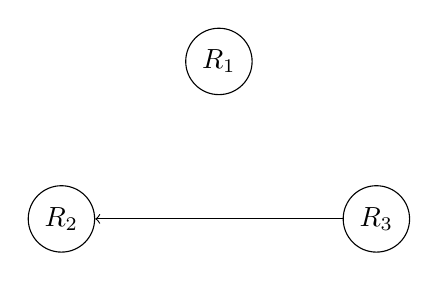
\begin{tikzpicture}[node distance=3cm]
\node[draw,circle] (11) at (2,0) {$R_1$};
\node[draw,circle] (02) at (0,-2) {$R_2$};
\node[draw,circle] (22) at (4,-2) {$R_3$};
\draw[->] (22) -- (02);
\end{tikzpicture}
\end{center}
\caption{Example of a bidirectional utility diagram over three attributes. \label{fig:biut}}
\end{figure}

\begin{example}
In Figure \ref{fig:biut} we present an example of a bidirectional diagram. This diagram includes only a directed edge and therefore represents the closest situation to a multilinear factorization, corresponding to a diagram with no edges. This diagram asserts that $R_1$ is \gls{UI} of $\{R_2,R_3\}$ and vice versa, plus that $R_3$ is \gls{CUI} of $R_2$ given $R_1$. Therefore, using the \gls{CUI} statements associated to the diagram in Figure \ref{fig:biut}, the general utility decomposition over three attributes in Example \ref{ex:genut} can be rewritten as
\begin{eqnarray*}
u&=&u(r_1^*,r_2^*,r_3^*)u(r_3\;|\;r_2^*)u(r_2\;|\; r_3^*)u(r_1)+
u(r_1^0,r_2^*,r_3^*)u(r_3\;|\;r_2^*)u(r_2\;|\; r_3^*)\hat{u}(r_1)+\nonumber\\
&&u(r_1^*,r_2^0,r_3^*)u(r_3\;|\;r_2^0)\hat{u}(r_2\;|\; r_3^*)u(r_1)+
u(r_1^*,r_2^*,r_3^0)\hat{u}(r_3\;|\;r_2^0)u(r_2\;|\; r_3^0)u(r_1)+\nonumber\\
&&u(r_1^0,r_2^0,r_3^*)u(r_3\;|\;r_2^0)\hat{u}(r_2\;|\; r_3^*)\hat{u}(r_1)+
u(r_1^0,r_2^*,r_3^0)\hat{u}(r_3\;|\;r_2^*)u(r_2\;|\; r_3^0)\hat{u}(r_1)+\nonumber\\
&&u(r_1^*,r_2^0,r_3^0)\hat{u}(r_3\;|\;r_2^0)\hat{u}(r_2\;|\; r_3^0)u(r_1).\label{eq:puiexample2}
\end{eqnarray*}
\end{example}

\citet{Abbas2010} identifies classes of bidirectional utility diagrams which give rise to optimal expansions of the multiattribute utility function, meaning that the conditional utility functions include the lowest number of arguments and that these do not need any consistency check. For the purposes of this thesis we consider only a subclass of bidirectional utility diagrams. 
\begin{definition}
\label{def:dirutdia}
We say that a bidirectional utility diagram is a \textit{directional utility diagram} if its graph is a \gls{DAG}.
\end{definition}
Note that the diagram in Figure \ref{fig:biut} is unconventional in the sense that an attribute is parent of another one having a lower index. We  motivate this choice in Chapter \ref{chapter4}, where such diagrams proves to be very useful.
\subsection{Univariate Utility Theory}
\label{sec:univariate}
In the previous sections we have shown how multiattribute utility problems can be decomposed into univariate ones when various sets of independences are believed to hold. We now discuss the characteristics of univariate utility functions and provide various examples. 

First, recall that utility functions are unique up to affine transformations, meaning that they imply the same preference ranking. Two such functions are said to be \textit{strategically equivalent}. In addition, \citet{Keeney1993a} showed that if two utility functions are strategically equivalent, then one must be an affine transformation of the other. 

We now introduce a variety of utility functions widely used in practice. 
\begin{example}
For the purposes of this example, we make explicit the dependence on the decision $\bm{d}$. Choices for $u_i(r_i,\bm{d})$ are 
\begin{itemize}
\item the \emph{zero-one utility}%
\begin{equation*}
\label{eq:01utility}
u_{i}(\bm{d},r_{i} )=\left\{
 \begin{array}{ll}
0,& \mbox{if } r_i\in B_{i}^{c}(\bm{d}), \\ 
1,& \mbox{if } r_i\in B_{i}(\bm{d}),
\end{array}
\right.
\end{equation*}%
where $B_{i}(\bm{d})$ is a region of the reward $R_{i}$ the \gls{DM} considers satisfactory under policy $\bm{d}\in\bm{\mathcal{D}}$, but otherwise it is not. Notice the only parameter here is the one defining the region $B_{i}(\bm{d})$;
\item the \emph{linear utility} function is 
\begin{equation*}
\label{eq:linearut}
u_i(r_i,\bm{d})= a(\bm{d})+b(\bm{d})r_i,
\end{equation*}
for $b(\bm{d})>0$;
\item the \emph{quadratic utility} 
\begin{equation*}
\label{eq:quadraticut}
u_{i}(\bm{d},r_{i} )=1-(\rho_{i}(\bm{d})r_{i})^{2},
\end{equation*}
 whose parameter is specified through the ideal scenario $\rho _{i}(d)$;
\item the \emph{polynomial utility} of degree $l$,
 \begin{equation*}
 \label{eq:polyut}
 u_i(\bm{d},r_i)=\sum_{j\in[l]}^l\rho_{ij}(\bm{d})r_i^j,
 \end{equation*}
where both the coefficients $\rho_{i,j}(\bm{d})$ and the domain of the rewards need to entertain some constraints \citep[see][for a discussion of these, which we omit here since are not relevant for our developments]{Keeney1993a,Muller1987}\footnote{Note that the polynomial utility has no monomial of degree zero. This is because many of the results of Chapter \ref{chapter5} are more easily interpretable in this case. Recall that adding such a monomial does not change the analysis as the two utilities are strategically equivalent.}; 
\item the \emph{exponential utility} function
\begin{equation*}
\label{eq:exput}
u_{i}(r_{i},\bm{d} )=1+\exp \left\{ -\rho _{i}(\bm{d})r_{i}\right\}, 
\end{equation*}
 where the parameter $\rho _{i}(\bm{d})>0$, reflects the degree of risk aversion (see below).
\end{itemize}
\end{example}

Many of the characteristics of a univariate utility function, as for example whether it is monotonic and convex or not, describe the preferences of the \gls{DM} and her attitude towards risk. See for more details on this \citet{Keeney1993a}.
\begin{comment}  
Utility functions are often in practice \textit{monotonic}. 
\begin{definition}
If $r_i>r_i^{'} \Longleftrightarrow u_i(r_i)>u_i(r_i^{'})$, then the utility function is monotonically increasing. If $r_i>r_i^{'} \Longleftrightarrow u_i(r_i)<u_i(r_i^{'})$, then the utility function is monotonically decreasing. Otherwise, it is non-monotonic.
\end{definition}

\begin{example}
The linear utility function in equation (\ref{eq:linearut}) is monotonically increasing, whilst the exponential in equation (\ref{eq:exput}) is monotonically decreasing. The quadratic utility function in equation (\ref{eq:quadraticut}) is nonmonotonic, but restricting its domain to the negative real line, then we can note that this utility is monotonically increasing.
\end{example}

As already mentioned, utility functions are further able to represent attitude towards risk. Consider for example two values $r_i$ and $r_i'$ of $R_i$ and a gamble yielding either of the two with equal probability. The expected utility of this gamble is $\bar{r}_i=(r_i+r_i')/2$. Suppose the \gls{DM} has the possibility to choose either to participate in the gamble or to receive $\bar{r}_i$ for sure. If she chooses the latter option, then she is actually stating that she prefers to avoid the risks associated to the gamble. In this case the \gls{DM} is said to be \textit{risk averse}. On the other end if she prefers participating in the gamble then she is said to be \textit{risk prone}. Lastly if she is indifferent between the two options then she is \textit{risk neutral}. The shape of the utility function is able to represent the \gls{DM}'s attitude towards risk.

\begin{proposition}
Let $u_i(r_i)$ be a monotonic utility function. The \gls{DM} is risk averse iff $u_i$ is concave, she is risk prone iff $u_i$ is convex and she is risk neutral iff $u$ is linear.
\end{proposition}

\begin{example}
Equation (\ref{eq:exput}) is the utility function of a risk prone \gls{DM}, whilst a \gls{DM} is risk averse if her utility is described by equation (\ref{eq:quadraticut}). A risk neutral \gls{DM} has the utility function in equation (\ref{eq:linearut}).
\end{example}

In order to measure the amount of risk aversion/proneness of a \gls{DM} we now introduce two quantities.

\begin{definition}
Let $u$ be a monotonically increasing utility function. The local risk aversion at $r_i$ is defined by
\begin{equation}
\label{eq:riskaversioninc}
q(r_i)=-\frac{\dr^2 u_i(r_i)}{\dr^2r_i}\left/\frac{\dr u_i(r_i)}{\dr r_i}\right..
\end{equation}
If $u$ is monotonically decreasing, the local risk aversion is defined as
\begin{equation}
t(r_i)=\frac{\dr^2 u_i(r_i)}{\dr^2r_i}\left/\frac{\dr u_i(r_i)}{\dr r_i}\right..
\label{eq:riskaversiondec}
\end{equation}
\end{definition} 

\begin{proposition}
If the local risk aversion functions $r$ and $t$ are positive for every $r_i$ the \gls{DM} is risk averse, whilst if these are negative for every $r_i$ the \gls{DM} is risk prone. If $r$ and $t$ are constantly equal to zero, the \gls{DM} is risk neutral.
\end{proposition}

\begin{example}
For the linear utility function of equation (\ref{eq:linearut}), the local risk aversion function is always equal to zero, confirming the risk neutrality. The local risk aversion function for the exponential utility of equation (\ref{eq:exput}) is $-\rho(d)$ which is negative for every $r_i$ and thus this function is risk prone. In addition we can note that the local risk aversion function is constant in $r_i$. Lastly consider the quadratic utility in equation (\ref{eq:quadraticut}) and restrict it to the negative line. The local risk averse function is equal to $-1/r_i$, which on the negative line is always positive: thus the \gls{DM} is risk averse in this case. Note also that in this case the local risk averse function is not constant, but it is an increasing function of $r_i$. In this case the \gls{DM} is said to be increasingly risk averse. 
\end{example}
\end{comment}

\section{Graphical Decision Models}
\label{sec:dec}
In the previous sections we assumed the existence of a generic decision space $\bm{\mathcal{D}}$ representing the available choices to a \gls{DM}. However in practice \glspl{DM} have to commit to a sequence of decisions, where some of the consequences of committing to a certain action are observed before having to choose subsequent policies. Such a sequential structure can be depicted through graphical representations of various types. Here we focus on the \acrfull{ID} model methodology, which can be thought of as an augmented version of a \gls{BN} including also decision and utility vertices. 
These are introduced in Section \ref{sec:id}. We  note that, although widely used in practice, \glspl{ID} are able to represent decision problems entertaining fierce symmetric conditions. In Section \ref{sec:asy} we provide a brief overview of the available models for the so called asymmetric decision problems.
 
For the purposes of this section, we slightly change our notation, which turns out to be very useful in concisely represent many of the features related to \glspl{ID}. An additional motivation to the use of this notation is mentioned in Section \ref{sec:symbolic}. This was introduced in \citet{Leonelli2015a}. We let $[n]$ be partitioned in $\mathbb{V}$ and $\mathbb{D}$, where $\mathbb{V}$ is the index set of the random (or non-controlled) variables, whilst $\mathbb{D}$ is the index set of the decisions (or controlled variables). 

\begin{example}
Let $n=6$ and assume $\mathbb{D}=\{1,4\}$ and $\mathbb{V}=\{2,3,5,6\}$. Then $Y_1$ and $Y_4$ are decisions, whilst $Y_2$, $Y_3$, $Y_5$ and $Y_6$ are random variables. 
\end{example}

\subsection{Influence Diagrams}
\label{sec:id}
As noted above, only decision problems enjoying strong symmetry conditions can be represented as \glspl{ID} \citep{Howard2005, Jensen2009,Smith2010}. We define here, following \citep{Smith2010}, the class of problems that entertains such a representation, that we call uniform.
\begin{definition}
\label{def:udp}
A \gls{UDP} is such that:
\begin{itemize}
\item a decision $Y_i$, $i\in \mathbb{D}$, is controlled before controlling $Y_j$, $j\in \mathbb{D}$, if $i<j$, and is remembered when making decisions with a higher index;
\item the space $\bm{\mathcal{Y}}_{[n]}$ is the product of the individual spaces, i.e. $\bm{\mathcal{Y}}[n]=\bigtimes_{i\in[n]}\mathcal{Y}_i$;
\item if a random variable $Y_i$, $i\in\mathbb{V}$, is observed before a variable $Y_j$, then $i<j$ and its distribution can depend  on $\bm{Y}_\mathbb{D}$ only through $\bm{Y}_{\mathbb{D}\cap[i{-1}]}$.
\end{itemize}
\end{definition}
The condition in the first bullet is usually referred to as no-forgetting. This bullet further implies that decisions are totally ordered. Furthermore decisions and random variables cannot be constrained with each other in \glspl{UDP}, as specified by the second bullet. The third bullet corresponds to the causal consistency lemma of \citet{Cowell1999a} and guarantees that decisions cannot influence variables that have been already observed.

As briefly mentioned, the vertex set of influence diagrams consists of random variables, decisions and utilities. We focus now on the latter type of nodes. The \gls{ID} literature usually assumes that there is an additive factorization between the utilities associated to different vertices. We refer to such \glspl{ID} as \glspl{AID}. In \citet{Leonelli2015a} we consider the much larger class of multiplicative utility factorizations and define the \gls{MID} which assumes this type of utility independences. In general it is possible to not assume any sort of independence and merge all the utility vertices into a unique vertex. This can be thought of, however, as a special case of an \gls{MID} with one only utility vertex. Therefore here we consider the class of \gls{MID} models. Let $U=\{u_i:i\in[m]\}$ and $u_i$, $i\in[m]$, maps a subspace $\bm{\mathcal{Y}}_{P_i}$ of $\bm{\mathcal{Y}}_{[n]}$ into $[0,1]$, with $P_i\subseteq [n]$.

\begin{definition}
\label{def:MID}
An  \gls{MID} $\Gr$  consists of
\begin{itemize}
\item a \gls{DAG} with vertex set $V(\Gr)=\{Y_1,\dots,Y_n,u_1,\dots, u_m\}$ and edge set $E(\Gr)$ including three types of edges defined by the following rules:
\begin{itemize}
\item for $i\in [m]$, $u_i$ has no children. Its parent set is $\{Y_j: j\in P_i\}$ and an index $i\in[n]$ can appear in a set $P_j$ only, $j\in[m]$, i.e. an element of $\{Y_1,\dots, Y_n\}$ is parent of at most one element of $U$. For any two $u_i$ and $u_j$, $i,j\in[m]$, $i>j$ if there is a $k\in P_i$ such that for every $l\in P_j$, $k>l$: i.e. a utility node $u_i$ has higher index than $u_j$ if one parent of $u_i$ has higher index than all parents of $u_j$;
\item for $i\in\mathbb{D}$, the parent set of $Y_i$, $\{Y_j: j\in \Pi_i\}$, for $\Pi_i\subset[n]$, consists of the variables, controlled and non-controlled, that are known when $Y_i$ is controlled;
\item for $i\in \mathbb{V}$, the parent set of $Y_i$,  $\{Y_j: j\in \Pi_i\}$, for $\Pi_i\subset[n]$, is such that $
Y_i \independent (\bm{Y}^i_{\{\mathbb{V}\setminus \Pi_i\}})| \bm{Y}_{\{\Pi_i\cap\mathbb{V}\}}$
for all instantiations of decisions preceding $Y_i$;\footnote{More succinctly this requirement can be written as $Y_i\independent \bm{Y}^{i}_{[n]}|\bm{Y}_{\Pi_i}$ using the notion of generalized conditional independence recently introduced in \cite{Dawid2014}.}
\end{itemize}
\item for $i\in\mathbb{V}$, a  density function $f_i(y_i|\bm{y}_{\Pi_i},\bm{\theta}_i)$; \footnote{Note that we allow densities to be conditional on controlled variables.}
\item a utility factorization $u$ assuming \gls{muia} $\bm{Y}_{P_i}$, $i\in[m]$.
\end{itemize}
\end{definition} 

Therefore in an \gls{MID} there are three types of vertices and three types of edges. The vertices are either random variables, decisions or utilities. Random variables are framed in circles, decisions in squares, whilst utilities have no framing in the \gls{DAG} $\Gr$ of an \gls{MID}. An edge into a vertex associated to a random variable asserts that the density of that random variable is conditional on the variable associated to the parent vertex. This edge therefore represents probabilistic dependence.\footnote{Probabilistic dependence can be associated to decisions since these can be thought of as random variables with degenerate probabilities having mass one in a point only.} Edges into decision vertices are called \textit{information} edges. These imply that the variable in the parent vertex is known when making that decision. Edges into utility vertices simply represent functional relationships, meaning that the utility is a function of the parent variables. \citet{Smith2010} defined the reduced \gls{ID}, where some of the information edges are not included, thus rendering the overall graphical representation clearer. Specifically, in a reduced \gls{ID} no edge $(Y_k,Y_i)$ is included if $(Y_k,Y_j)\in E(\Gr)$, $j<i$, $j,i\in\mathbb{D}$. 

Similarly to \glspl{BN}, \glspl{ID} are extremely powerful graphical representations of the qualitative structure underlying the elements of decision problems. In particular, these are able to depict both continuous and discrete domains. Note that although $P_i$, $i\in [m]$, is effectively the index parent set, we had to use a different notation than the one generically introduced for graphs in Appendix $\ref{appendixB}$, because of the existence of both utility and non-utility nodes.

Definition \ref{def:MID} implies a total order on the vertex set of an \gls{MID}. For $i\in[m]$, let $j_i$ be the highest index of $P_i$ and $\mathbb{J}=\{j_1,\dots, j_m\}$. The totally ordered sequence associated to $V(\Gr)$ is called \textbf{\gls{DS}} of the \gls{MID} $\Gr$ and  indicated as   $S:=(Y_1,\dots,Y_{j_1},u_1,Y_{j_1+1},\dots,Y_{j_m},u_m)$.  In distinction with other authors \citep[e.g.][]{Jensen2009,Cowell1999a}, we do not introduce utility nodes only at the end of the \gls{DS}. This allows for a computationally efficient computation of the expected utility scores, since optimal decisions can be shown to be functions of smaller sets of preceding variables.

\begin{example}
Figure \ref{fig-ex} presents an \gls{MID} with vertex set $\{Y_1,\dots, Y_6, u_1,\dots, u_3\}$ describing a gross simplification of the possible countermeasures after an accident at a nuclear power plant. For this \gls{MID}, $n=6$, $m=3$, $\mathbb{D}=\{1,4\}$ and $\mathbb{V}=\{2,3,5,6\}$. Therefore, there are two controlled variables $Y_1$ and $Y_4$: the first consisting of the possibility of closing down the power plant, the second of evacuating the nearby population. Before controlling $Y_4$, the variables $Y_1$, $Y_2$ and $Y_3$ are observed since $\Pi_4=\{1,2,3\}$.
 There are four random nodes: $Y_2$ and $Y_3$ measure the amount of dispersion of the contaminant in the atmosphere and to the ground respectively, $Y_5$ estimates the human intake of radiation and $Y_6$ ranks the level of stress in the population. This \gls{DAG} implies for example that $Y_5\independent Y_2\;|\;Y_3$ for every $y_1\in\mathcal{Y}_1$ and $y_4\in\mathcal{Y}_4$. The variable $Y_5$ has parent set $\{Y_i: i\in \Pi_5\}$ where $\Pi_5=\{3,4\}$ and $\Pi_{5\cap\mathbb{V}}=\{3\}$. We further assume all the variables to be binary, taking values in the spaces $\mathcal{Y}_i=\{1,0\}$, $i\in [6]$. When $\mathcal{Y}_i$ is associated to a decision node, 1 and 0 correspond to, respectively, proceed and not proceed. If  $\mathcal{Y}_i$ is associated to a random node, then 1 and 0 correspond respectively to high and low.
  The \gls{MID} definition is completed by three utility nodes, $u_1$, $u_2$ and $u_3$. For example the set $P_3$ is equal to $\{4,6\}$ and therefore $Y_4$ and $Y_6$ are the arguments of the utility function $u_3$. Lastly, the  \gls{DS} $(Y_1,Y_2,Y_3,u_1,Y_4,Y_5,u_2,Y_6,u_3)$ is the one associated to the \gls{MID} in Figure \ref{fig-ex}, where $j_1=3$, $j_2=5$, $j_3=6$ and $\mathbb{J}=\{3,5,6\}$.  
\end{example}

\begin{figure}
\vspace{0.8cm}
\centerline{
\xymatrix{
*+[F]{Y_1}\ar@/^2pc/[rr]\ar[r]\ar[rd]&*+[Fo]{Y_3}\ar[dl]\ar@/^2pc/[rr]\ar[r]&*+[F]{Y_4}\ar[d]\ar[r]\ar[rd]&*+[Fo]{Y_5}\ar[r]\ar[d]&u_2\\
u_1&*+[Fo]{Y_2}\ar[u]\ar[ru]&u_3&*+[Fo]{Y_6}\ar[l]&
}
}
\vspace{0.2cm}
\caption{An influence diagram describing the available countermeasures after an accident at a nuclear power plant.}
\label{fig-ex}
\end{figure}

The density function associated to an \gls{MID} entertains a factorization which mirrors the one in Lemma \ref{lemma:rec}.

\begin{lemma}
\label{lemma:id}
The probability density function associated to an \gls{MID} can be written as
\begin{equation*}
f(\bm{y}_{\mathbb{V}}\;|\;\bm{\theta})=\prod_{i\in{\mathbb{V}}}f(y_i\;|\;\bm{y}_{\Pi_i},\bm{\theta}_i),
\end{equation*}
where $\bm{\theta}^\T=(\bm{\theta}_i)_{i\in\mathbb{V}}$.
\end{lemma}

\begin{example}
The density function associated to the \gls{MID} in Figure \ref{fig-ex} can be written as
\begin{equation*}
f(\bm{y}\;|\;\bm{\theta})=f(y_2\;|\;y_1,\bm{\theta}_2)f(y_3\;|\;y_2,y_1,\bm{\theta}_3)f(y_5\;|\;y_4,y_3,\bm{\theta}_5)f(y_6\;|\;y_5,y_4,\bm{\theta}_6).
\end{equation*}
The utility factorization associated to this \gls{MID} coincides with the one in equation (\ref{eq:examplemultilinear})
\end{example}
\subsubsection{Evaluation of Influence Diagrams.} 
To evaluate an \gls{MID} means to identify a sequence of optimal decisions maximizing the expected utility function. However, only  \glspl{MID} whose topology is such that, for any index $j\in\mathbb{D}$, the only variables that are known at the time the \gls{DM} makes a decision $Y_j$  have an index lower than $j$, can be directly evaluated \citep{Smith1989a}. This is because the evaluation outputs optimal decisions as functions of observed quantities only and therefore \glspl{DM} can unambiguously commit to such an optimal course of action. Here we define this class using the terminology of \cite{Smith2010}.
\begin{definition}
\label{ei}
An \gls{MID} $\Gr$  is said to be in extensive form if $Y_i$ is a parent of $Y_j$, $j\in\mathbb{D}$, for all $i<j$. 
\end{definition}
We assume here for the sake of simplicity that the \gls{MID} under study is in extensive form. However, we note here that any \gls{MID} in non extensive form can be transformed into an extensive form one. There are several rules, which we do not introduce here, to manipulate the topology of an \gls{MID}, as for example, edge reversal and barren node removal \citep[see e.g.][]{Jensen2009}, such that the resulting \gls{MID} is in extensive form.  Without restriction we also assume that every vertex $Y_i$ of the \gls{MID}, $i\in [n]$, has at least one child. Random and controlled vertices with no children could be simply deleted from the graph without changing the outcome of the evaluation of the \gls{MID} \citep[see e.g.][]{Jensen2009}.  

\begin{example}
The \gls{MID} in Figure \ref{fig-ex} is in extensive form since $\Pi_4=\{1,2,3\}$. If either the edge $(Y_2,Y_4)$ or $(Y_3,Y_4)$ were deleted from this diagram then the \gls{MID} would not be in extensive form any more. Furthermore note that the only vertices with no children are $u_1$, $u_2$ and $u_3$. 
\end{example}

Several algorithms have now been defined to evaluate \glspl{ID}. These can work directly on the \gls{ID} \citep{Shachter1986,Olmsted1983}, transform it into a decision tree \citep{Canbolat2007}, or convert the diagram into some other graphical structure \citep{Jensen1994,Madsen1999}. There were severe computational issues related to the evaluation of \glspl{ID}, but there are now several  promising methodologies designed to overcome these challenges, as noted in \citet{Bielza2011} and \citet{Gomez2007}. Many different pieces of software are also now available to build and automatically evaluate large \glspl{ID} \citep{Jensen2013}. The simplest way to evaluate an \gls{MID} in extensive form is through a backward inductive algorithm over the vertices of the \gls{DAG} \citep[see e.g.][]{Jensen2009}. Here we introduce a computationally efficient version of this algorithm, including at each step only the strictly necessary utility nodes. For simplicity we work with the predictive distribution $f(\bm{y})=\int_{\bm{\Theta}}f(\bm{y}\;|\;\bm{\theta})f(\bm{\theta})$, but the result can be straightforwardly generalized to take into account the parameter vector.  The identification of the optimal policy is based on the computation of the functions $\bar{u}_i(\bm{y}_{B_i})$, $i\in[m]$, we formally introduce in Proposition \ref{i-th}, where 
\begin{equation*}
\label{Ai}
B_i=\left\{\bigcup_{\substack{k\geq i\\ k\in\mathbb{V}}}\Pi_k\bigcup\bigcup_{\substack{j\geq i\\j\in\mathbb{J}}}P_j\right\}\setminus\{i,\dots,n\},
\end{equation*}
is the set including the indices of the variables that appear as arguments of $\bar{u}_i$. It can be noted that $B_i$ includes only indices smaller than $i$ that are either in the parent set of a random variable $Y_k$, $k>i$, or in a set $P_j$ such that $u_j$ succeeds $Y_i$ in the \gls{DS} of the \gls{MID}.

\begin{example}
We compute here the sets $B_5$ and $B_4$ associated with the \gls{MID} in Figure \ref{fig-ex}. The set $B_5=\{3,4\}$ since $B_5=\{\Pi_6\cup \Pi_5\cup P_3\cup P_2\}\setminus\{5,6\}$, where $\Pi_6=\{4,5\}$, $\Pi_5=\{3,4\}$, $P_3=\{4,6\}$ and $P_2=\{5\}$. Furthermore $B_4=\{3\}$ since it can be noted that $B_4=B_5\setminus \{4\}$.
\end{example}

\begin{proposition}
\label{i-th}
The optimal decision associated to an \gls{MID} yields expected utility $\bar{u}_1(\bm{y}_{B_1})$, where, for $i\in[n]$, $\bar{u}_i(\bm{y}_{B_i})$ is defined as
\begin{equation*}
\label{eq:id1}
\bar{u}_i(\bm{y}_{B_i})=\left\{
\begin{array}{lcl}
\bar{u}_i^{\mathbb{D}}(\bm{y}_{B_i}),&&\mbox{if } i\in\mathbb{D},\\
\bar{u}_i^{\mathbb{V}}(\bm{y}_{B_i}),&&\mbox{if } i\in\mathbb{V}
\end{array}
\right.
\end{equation*}
where, for $i=n$,
\begin{align}
&\bar{u}_n^{\mathbb{D}}(\bm{y}_{B_n})=\max_{\mathcal{Y}_n}k_mu_m(\bm{y}_{P_m}),\hspace{1cm }\bar{u}_n^{\mathbb{V}}(\bm{y}_{B_n})=\int_{\mathcal{Y}_n}k_mu_m(\bm{y}_{P_m})f_n(y_n\;|\;\bm{y}_{\Pi_n})\dr y_n,\label{cond4}\\
\intertext{and, for $i\in[n-1]$, if $i\in \mathbb{J}$ and assuming $i\in P_l$,}
&\bar{u}_i^{\mathbb{D}}(\bm{y}_{B_i})=\max_{\mathcal{Y}_i}\Big(hk_lu_l(\bm{y}_{P_l})\bar{u}_{i+1}(\bm{y}_{B_{i+1}})+k_lu_l(\bm{y}_{P_l})+\bar{u}_{i+1}(\bm{y}_{B_{i+1}})\Big),\label{cond2}\\
&\bar{u}_i^{\mathbb{V}}(\bm{y}_{B_i})=\int_{\mathcal{Y}_i}\Big(hk_lu_l(\bm{y}_{P_l})\bar{u}_{i+1}(\bm{y}_{B_{i+1}})+k_lu_l(\bm{y}_{P_l})+\bar{u}_{i+1}(\bm{y}_{B_{i+1}})\Big)f_n(y_n\;|\;\bm{y}_{\Pi_n})\dr y_n\label{cond3},\\
\intertext{whilst, if $i\not\in\mathbb{J}$,}
&\bar{u}_i^{\mathbb{D}}(\bm{y}_{B_i})=\max_{\mathcal{Y}_i}\bar{u}_{i+1}(\bm{y}_{B_{i+1}}),\hspace{1cm}\bar{u}_i^{\mathbb{V}}(\bm{y}_{B_i})=\int_{\mathcal{Y}_i}\bar{u}_{i+1}(\bm{y}_{B_{i+1}})f_i(y_i\;|\;\bm{y}_{\Pi_i})\dr y_n.\label{cond1}
\end{align}
\end{proposition}
The proof of this result is given in Appendix \ref{appendixA1}.
Note that in equation (\ref{cond4}), the argument of both $\bar{u}_n^{\mathbb{D}}$ and $\bar{u}_n^{\mathbb{V}}$ is $\bm{y}_{P_m}$ since, by construction, $Y_n$ is a parent of $u_m$.

\begin{comment}
\subsubsection{Modifications of Influence Diagrams.}

\label{sec:topology}

Proposition \ref{i-th} assumes that the \gls{MID} is in extensive form and that it can be straightforwardly evaluated to compute expected utility scores. In practice it has been recognized that typically a \gls{DM}  builds an \gls{MID} so that variables and decisions are ordered in the way they actually happen. However this might not correspond to the order in which variables are observed. Thus, \glspl{MID} often are not in extensive form and, for this reason, they need to be transformed. It is always possible to transform a diagram into one in extensive form, although this might entail the loss of conditional independence structure. Following \citet{Shachter1986}, the two rules we study here to manipulate non extensive diagrams are the so called \textbf{arc reversal} and \textbf{barren node removal}. These are often used in combination by first reversing the direction of some edges of the \gls{MID} and then removing a vertex that, consequently to the reversals, becomes barren, i.e. has no children. 

\begin{proposition}
\label{manipulation}
The evaluation of an \gls{MID} $\Gr'$ provides the same optimal policy as the one deduced from an \gls{MID} $\Gr$ if the following manipulations are implemented:
\begin{itemize}
\item \textbf{Arc Reversal}: reverse the edge $(Y_i,Y_j)$ into $(Y_j,Y_i)$, if $Y_i$ is the father of $Y_j$ in $\Gr$, $i,j\in\mathbb{V}$, and change the edge set as 
\begin{equation}
E(\Gr')=E(\Gr)\setminus \big\{(Y_i,Y_j)\big\}\cup \big\{(Y_j,Y_i)\big\}\cup C_i' \cup C_j',
\end{equation}
where 
\begin{equation}
C_i'= \big\{(Y_k,Y_i), \forall\; k\in\{\Pi_j\setminus \{i\}\}\big\}, \;\;\;\mbox{ and } \;\;\; C_j'=\cup\big\{(Y_k,Y_j), \forall\; k\in \Pi_i\big\},
\end{equation}
\item \textbf{Barren Node Removal}: remove the vertex $Y_i$, for $i\in\mathbb{V}$, if this has no children and transform the diagram according to the following rules:
\[
V(\Gr')=V(\Gr)\setminus \{Y_i\},\;\;\;\;\hspace{0.5cm}E(\Gr')=E(\Gr)\setminus \big\{(Y_k,Y_i): \forall \; k \in \Pi_i \big\}.
\]
\end{itemize}
\end{proposition}
We described an arc reversal between two random vertices only in the case when one is the father of the other. However, this assumption is not restrictive since, if there is one edge to reverse in order to make a vertex barren, then one node of the edge must be the father of the other. 


\begin{figure}
\begin{center}
\subcaptionbox{A variant of the MID of Figure \ref{fig-ex} without  $(Y_2,Y_4)$\label{fig-ex1}}
[.49\linewidth]{
\xymatrix{
U_1&*+[Fo]{Y_3}\ar[l]\ar[dd]\ar[dr]&*+[Fo]{Y_2}\ar[l]&*+[F]{Y_1}\ar[dl]\ar[l]\ar@/^1pc/[ll]\\
&&*+[F]{Y_4}\ar[d]\ar[dl]\ar[rd]&\\
U_2&*+[Fo]{Y_5}\ar[r]\ar[l]&*+[Fo]{Y_6}\ar[r]&U_3
}}
\subcaptionbox{Reversal of the edge $(Y_2,Y_3)$ from the MID of Figure \ref{fig-ex1}.\label{fig-ex2}}
[.49\linewidth]{
\xymatrix{
U_1&*+[Fo]{Y_3}\ar[l]\ar[dd]\ar[dr]\ar[r]&*+[Fo]{Y_2}&*+[F]{Y_1}\ar[dl]\ar[l]\ar@/^1pc/[ll]\\
&&*+[F]{Y_4}\ar[d]\ar[dl]\ar[rd]&\\
U_2&*+[Fo]{Y_5}\ar[r]\ar[l]&*+[Fo]{Y_6}\ar[r]&U_3
}}
\caption{Example of an  edge reversal in a non extensive form MID. }\label{fig:1}
\end{center}
\end{figure}

\begin{figure}
\centerline{
\xymatrix{
U_1&*+[Fo]{Y_3}\ar[l]\ar[dd]\ar[dr]&&*+[F]{Y_1}\ar[dl]\ar@/^1pc/[ll]\\
&&*+[F]{Y_4}\ar[d]\ar[dl]\ar[rd]&\\
U_2&*+[Fo]{Y_5}\ar[r]\ar[l]&*+[Fo]{Y_6}\ar[r]&U_3
}}
\caption{MID resulting from both the barren node removal of $Y_2$ from the MID of Figure \ref{fig-ex2} and the application of the sufficiency theorem for the MID of Figure \ref{fig-ex1} \label{fig-ex3}}
\end{figure}

\begin{example}
The process of transforming a non extensive form \gls{ID} into an extensive form one is exemplified in Figures \ref{fig-ex2} and \ref{fig-ex3} for the \gls{MID} in Figure \ref{fig-ex1}, a non-extensive variant of the \gls{MID} in Figure \ref{fig-ex} not including the edge $(Y_2,Y_4)$. In Figure \ref{fig-ex2} we report the \gls{MID} resulting from the reversal of the edge $(Y_2,Y_3)$ and in Figure \ref{fig-ex3} the network in extensive form obtained by deleting the barren node $Y_2$. 
\end{example}


The above rules  enable an  \gls{MID} to be transformed into one in extensive form. However, an extensive form diagram can be further manipulated to simplify its evaluation. In practice  \glspl{DM} often also include in the \gls{MID} variables that subsequently turn out  not to be strictly necessary to identify an optimal policy.  \glspl{DM} are able to provide probabilistic judgements for conditional probability tables associated to an \gls{MID} which includes variables describing the way they understand the unfolding of events. However their understanding usually includes variables that are redundant for the evaluation of the \gls{MID}. A modification of the \gls{DAG} $\Gr$ of an \gls{MID} which identifies only the strictly necessary variables for the identification of an optimal policy is  via the \textit{sufficiency principle} \citep[see][]{Smith1989a, Smith1989}, which mirrors the concept of sufficiency in statistics and is based on the concept of d-separation of Section \ref{sec:BN}. 

\begin{proposition}
\label{suff}
For a $j\in \mathbb{D}$, supposed $Y_i$ is such that $i\in \mathbb{V}\cap \Pi_i$. Then if $Y_i$ is d-separated from $\{U_k, \mbox{ for } k \; s.t. \; i\leq j_k\}$ by $\{\bm{Y}_k: k\in \{\Pi_i\setminus \{i\}\}\}\cup \{Y_k:k\in\mathbb{D}\}$ in the \gls{MID} $\Gr$, then the evaluation of the graph $\Gr'$ provides the same optimal policy as $\Gr$, where $\Gr'$ is such that 
\begin{align}
&V(\Gr')=V(\Gr)\setminus \{Y_i\},\\
&E(\Gr')=E(\Gr)\setminus \{(Y_i,Y_j), \; \forall\; j\in Ch_i\}\setminus \{(Y_k,Y_i),\;\forall\; k\in \Pi_i\}\cup C_i,
\end{align}
where 
\begin{equation}
C_i=\{(Y_k,Y_j),\; \forall \; j\in Ch_i,\;\forall\; k \in \Pi_i\}.
\end{equation}
\end{proposition}
For simplicity here, we stated the sufficiency principle concerning a single vertex $Y_i$. This principle can be more generally defined for a vector of variables \citep[see][]{Smith1989a, Smith1989}. However, we can simply apply the criterion we introduced in Proposition \ref{suff} for each variable of the vector and obtain the same result. 

\begin{example} 
Consider the \gls{MID} in Figure \ref{fig-ex}. For this diagram, its moralization does not add any edge. Any path from $Y_2$ into $U_i$, $i\in[3]$, has to pass through both $Y_3$ and $Y_4$. Thus, according to Proposition \ref{suff}, we can delete $Y_2$ and modify the diagram to obtain the one in Figure \ref{fig-ex3}. For this example this network corresponds  to the same one resulting from the reversal of the arc $(Y_2,Y_3)$ and the deletion of $Y_2$. However in general this does not have to be the case. 
\end{example}
\end{comment}

\subsection{Asymmetric Models}
 \label{sec:asy}
In the introduction we noted that the \gls{ID} framework is able to represent \glspl{UDP} only. However, real decision problems often exhibit asymmetries of various kinds. In \citep{Jensen2009} asymmetries are categorized in three classes. If the possible outcomes or decision options of a variable vary depending on the past, the asymmetry is called \textit{functional}. If the very occurrence of a variable depends on the past, the asymmetry is said to be \textit{structural}. \textit{Order} asymmetries are present if $\bm{Y}_{\mathbb{D}}$ is not totally ordered.

We note here that there are four types of functional asymmetries that can occur:
\begin{itemize}
\item \textbf{chance} $\rightarrow$ \textbf{chance}: the outcome of random variables restricts the outcomes of other random variables;
\item \textbf{chance} $\rightarrow$ \textbf{decision}: the outcome of random variables restricts the options of controlled variables;
\item \textbf{decision} $\rightarrow$ \textbf{chance}: decisions taken restrict the possible outcomes of random variables;
\item \textbf{decision} $\rightarrow$ \textbf{decision}:  decisions taken restrict the options of other controlled variables.
\end{itemize}
Heuristically, for each of these asymmetries the observation of $\bm{y}_A$, $A\subset [n]$, changes the space $\bm{\mathcal{Y}}_B$ associated to a vector $\bm{Y}_B$, such that $A\cap B=\emptyset$. This new space, $\bm{\mathcal{Y}}_B'$ say, is a subspace of $\bm{\mathcal{Y}}_B$.

The simplest solution to the representation of an asymmetric problem is by embedding it in a symmetric one which can be represented as an \gls{ID}. The above mentioned evaluation algorithms can then be used to identify optimal solutions in the embedded version of the problem. 

Clearly this methodology has several drawbacks. Most importantly it does not graphically represent the relevant asymmetries and often considers a much larger problem space than the original one. For this reason a variety of graphical models have been introduced to represent a variety of asymmetric constraints \citep{Smith1993,  Demirer2006a, Nielsen2003, Jensen2006, Jensen2002, Bhattacharjya2012}. It is not the purpose of this thesis to review these models and we briefly illustrate part of the semantic of the sequential \gls{ID} \citep{Jensen2006} model in the following example. 

\begin{example}
\label{eee}
Consider the \gls{ID} in Figure \ref{fig-ex} and assume that the \gls{DM} now believes her decision problem is characterized by the following three asymmetries:
\begin{itemize}
\item whenever she decides to close the power source, then the population cannot be evacuated from the area: $Y_1=1\Rightarrow Y_4=0$;
\item if either the deposition or the dispersion levels in the area are high, then  the human intake is high: $Y_2=1 \lor Y_3=1\Rightarrow Y_5=1$;
\item if the evacuation option is followed then both the human intake and the stress levels in the population are high: $Y_4=1\Rightarrow Y_5=1 \land Y_6=1$.
\end{itemize}

\begin{figure} 
\begin{center}
\begin{tikzpicture}[node distance=4cm]
\node[draw,rectangle] (00) at (0,0) {$Y_1$};
\node[draw,circle] (1-1) at (2,-1) {$Y_3$};
\node[draw,circle] (11) at (2,1) {$Y_2$};
\node[draw,rectangle] (20) at (4,0) {$Y_4$};
\node[draw,circle] (31) at (8,1) {$Y_6$};
\node[draw,circle] (3-1) at (8,-1) {$Y_5$};
\node (0-1) at (0,-1) {$U_1$};
\node (21) at (4,1) {$U_3$};
\node (4-1) at (10,-1) {$U_2$};
\draw[->] (00) -- (11);
\draw[->] (00) -- (1-1);
\draw[->,anchor=center, below] ([yshift=0.1cm]00.east) to node {} ([yshift=0.1cm]20.west);
\draw[->,dashed,anchor=center, below] ([yshift=-0.1cm]00.east) to node {\tiny{$Y_1=4|Y_4=0$}} ([yshift=-0.1cm]20.west);
\draw[->] (11) -- (1-1);
\draw[->] (1-1) -- (0-1);
\draw[->] (20) -- (21);
\draw[->] (31) -- (21);
\draw[->] (3-1) -- (4-1);
\draw[->] (11) -- (20);
\draw[->] (1-1) -- (20);
\draw[->] (1-1) -- (3-1);
\draw[->,anchor=center, below] (20.north) to node {} (31);
\draw[->,anchor=center, below] (20.south) to node {} (3-1);
\draw[->] (3-1) -- (31);
\node[draw=black, dashed, ellipse, inner sep =4pt, fit= (11) (1-1)] (circ1) {};
\node[draw=black, dashed, ellipse, inner sep =4pt, fit= (31) (3-1)] (circ2) {};
\draw[->, dashed,anchor=center, below] ([yshift=-1.2cm]circ1.east) to node {\tiny{$Y_2=1,Y_3=1|Y_5=1$}} ([yshift=-0.2cm]3-1.west);
\draw[->, dashed,anchor=center, above] (20) to node {\tiny{$Y_4=1|Y_5=1,Y_6=1$}} (circ2.west);
\end{tikzpicture}
\end{center}
\caption{Representation of the asymmetric version of the MID of Figure \ref{fig-ex} through a sequential influence diagram. }\label{sid}
\end{figure}
Our graphical representation of these asymmetries is given in Figure \ref{sid}, corresponding to a sequential influence diagram \citep{Jensen2006}. Asymmetries are represented as labels on additional dashed arcs. If the asymmetry is composite, meaning that it involves more than two variables, then vertices can be grouped through a dashed ellipse and dashed arcs can either start or finish by the side of these ellipses. 
\end{example} 

As exemplified by the diagram in Figure \ref{sid}, the graphical representation of asymmetric decision problems, although providing a framework to quickly identify optimal policies, often lose the intuitiveness and the clarity of representation of standard \glspl{ID}. We will discuss more extensively this issue in Section \ref{sec:symbolic}.
 
Asymmetric decision problems can also be explicitly modelled as \textit{decision trees} \citep[see e.g.][]{Clemen1996a,French2009}, an augmented version of an event tree including decision vertices and whose leaves are utilities. These suffer the same drawbacks of staged and event trees. Recently \citet{Cowell2010} introduced the decision \gls{CEG} which can more compactly represent asymmetric decision problems and shares the same features of the \gls{CEG} model class.
 
\section{Group Decision Making}
\label{sec:group}
The \gls{SEU} model characterizes rational decision making for single \glspl{DM}. However in practice most decisions in organizations and society are responsibility of groups rather than individuals: juries, cabinets and boards of directors are some examples. In addition, even single \glspl{DM} rarely commit to certain courses of actions without seeking for the help of appropriate experts. How the suggestions of various experts have to be reconciled is a very interesting question and a variety of solutions have been proposed. Following \citet{French2011} we identify two main contexts of group decision making:
\begin{itemize}
\item the \textbf{group decision problem}: a group of individuals is jointly responsible and accountable for the decision;
\item the \textbf{expert problem}: a group of experts are consulted by a single \gls{DM} who is responsible and accountable for the decision to be made.
\end{itemize}
\citet{French2011} also identifies the \textit{textbook problem} context which for the purposes of this thesis is not discussed here. Note further that a combination of the two above scenario can be considered in practice.

For ease of notation we again leave the dependence on the parameter vector $\bm{\theta}$ implicit. 
 
\subsection{The Group Decision Problem}
\label{sec:groupdecprob}
Suppose there are $m$ \glspl{DM}, each of them having a subjective probability distribution $f^i(\bm{y})$ over some quantity of interests $\bm{y}$ and a utility function $u^i(\bm{d},\bm{r})$. Note that here the index $i$ refers to the $i$-th \gls{DM}. We assume each of them to behave as a Bayesian expected utility maximizer. Following \citet{French2009} and  \citet{French2011} we identify four approaches to describe how a collaborative group of \glspl{DM} might act rationally:
\begin{enumerate}
\item combine each $f^i(\bm{y})$ and each $u^i(\bm{d},\bm{r})$, $i\in [m]$, into respectively a group probability and utility function:
\begin{equation*}
f^g(\bm{y})=T^p(f_1,\dots,f_m),\;\;\;\;\; u^g(\bm{d},\bm{r})=T^u(u_1,\dots,u_m),
\label{eq:approach11}
\end{equation*}
for some functions $T^p$ and $T^u$ such that $f^g$ and $u^g$ are respectively density and utility functions. Then the group ranks decisions according to the group expected utility function
\begin{equation*}
\label{eq:approach12}
\E(u^g(\bm{d}))=\int_{\bm{\mathcal{R}}} u^g(\bm{d},\bm{r})f^g(\bm{y})\dr \bm{y};
\end{equation*}
\item each \gls{DM} individually ranks the decisions according to her expected utility 
\begin{equation*}
\label{eq:approach2}
\E(u^i(\bm{d}))=\int_{\bm{\mathcal{R}}} u^i(\bm{d},\bm{r})f^i(\bm{y})\dr \bm{y},
\end{equation*}
and then votes according to this ranking. A group choice is then made according to the individual votes;
\item a \textit{supra\gls{DM}} is imagined to exist who observes the values and beliefs of each \gls{DM} and then altruistically uses this knowledge to develop a unique expected utility function for the group;
\item the group gathers in a facilitated meeting and discusses the issue until consensual agreement on the form of both the probability distribution and the utility function is found. An optimal decision is then reached by consensus.
\end{enumerate}

A few comments are necessary here. Point 1 requires the identification of, or better an agreement on, the functions $T^p$ and $T^u$ to pool the beliefs and the preferences of the \glspl{DM}. We discuss extensively about the functions $T^p$ in Section \ref{sec:expert}, whilst we do not explicitly deal with possible solutions for $T^u$ \citep[see for more details ][]{Keeney1976, Keeney1993a, Keeney2013}.  

Point 2 assumes the group is able to identify a voting system embedding some concept of democracy. However, as shown first by \citet{Arrow1963} and from several authors after him, any algorithmic method of combining votes of \glspl{DM} is subject to paradoxes and inconsistencies. Therefore democratic voting for group is in general not possible. The implications of these results further implies that the methods of point 1 in the list above exhibit the same sort of inconsistencies.

The recognition of the non existence of rational democratic voting led to the idea that group decisions making is a flawed concept. Individuals make decisions, groups do not. Therefore group decision making is now better viewed as a social process during which the beliefs and preferences of the group's members are translated into a course of action \citep{French2009}. For this reason research in this area moved from mathematical methods to behavioural ones, corresponding to point 4 of the list above. We review such literature in the next section.

Before that, we note that recently \citet{Keeney2013} introduced a new set of axioms describing rationality in groups of \glspl{DM}. Under these axioms it was shown that the group expected utility is simply a linear combination of the individual \glspl{DM}' expected utilities, where the weights need to be jointly agreed.    

\subsection{Decision Conferencing}
\label{sec:decconf}
\textit{Decision conferences} and \textit{facilitated workshops} are the most common techniques of behavioural aggregation of \glspl{DM}' beliefs and preferences \citep{ Ackermann1996,Phillips1984,Phillips1993}. These are usually two days events with around fifteen participants \citep[although for example in the Chernobyl project we discussed in Chapter \ref{chapter1} the number of participants was way larger as noted in][]{French2009}.

In such meetings, a \textit{facilitator}, an individual skilled in the process of group discussion, encourages debate among the \glspl{DM} and keeps the group's focus on the issue at hand. The facilitator is usually not an expert of the problem to be examined and has no ownership of the decision to be made. 

Each \gls{DM} often has available interactive software to run her own analyses and observe the results of others' beliefs, which are also projected in the room. This software uses decision models which result fundamental to foster discussion and raise the main issues that need to be investigated by the group. The results of sensitivity analyses are also shown to the \glspl{DM} in order to build consensus and avoid debates on irrelevant alternatives or parameters that do not affect the group's course of action. 

As we discussed in Chapter \ref{chapter1}, these types of meetings resulted fundamental within the Chernobyl Project. The discussions at those meetings are summarized in \citet{French2009} and \citet{Smith2010}. \citet{Ackermann1996} reports more than 100 of successful applications of such behavioural techniques. 

A different method called \textit{Delphi protocol} has been designed to reach consensus by the remote and electronic compilation of a series of questionnaire, thus not requiring the group to meet \citep{Dalkey1963,Linstone1975}. Under this protocol each individual anonymously responds to the questionnaire. The answers are then sent to the other members for further comments and generations of possible courses of actions. This sequence is then iteratively repeated until consensus is reached. 
 
\subsection{The Expert Problem}
\label{sec:expert}

The second context where groups are involved in the decision making process is the expert problem. Here an individual \gls{DM} needs to synthesize the beliefs of a group of $m$ experts into a unique probability distribution. Following \citet{Clemen99} and \citet{French2011}, we identify  two main categories of approaches to deal with this problem:
\begin{itemize}
\item \textit{behavioural}: the group reaches consensus through discussion as described in Section \ref{sec:decconf};
\item \textit{mathematical}: a unique probability distribution is built from the ones elicited individually by each expert through some algorithmic rule. 
\end{itemize}
We focus now on mathematical methods, which again can be broadly categorized into two main branches. Before introducing the details of these approaches, we remark that it is not the scope of this thesis to explore the validity of each of these \citep[see e.g.][and the references therein for an extensive discussion]{Clemen99,French2011}. \citet{O'Hagan2006a} discusses  protocols to be followed by each expert to elicit his own probability distribution, whilst \citet{Merrick2008} introduces methods to identify the right mix of experts to obtain the best aggregated belief.

\subsubsection{The Bayesian Approach.}
The \textit{Bayesian} approach treats experts' judgements as data, synthesized in some appropriate likelihood function, to update the prior probability of the \gls{DM}. Let $\bm{y}$ be the quantity of interest to the \gls{DM} and $\bm{e}=(e_1,\dots,e_m)$ be the beliefs of the experts about $\bm{y}$. Then the \gls{DM}'s belief about $\bm{y}$ taking into account the experts' judgements, $f(\bm{y}\;|\; \bm{e})$ say, can be derived by applying equation (\ref{eq:bayes}) as
\begin{equation*}
\label{eq:bayesianaggregation}
f(\bm{y}\;|\; \bm{e})\propto f(\bm{e}\;|\; \bm{y})f(\bm{y}),
\end{equation*}
where $ f(\bm{e}\;|\; \bm{y})$ is the likelihood function representing the \gls{DM}'s confidence in the experts and $f(\bm{y})$ is the \gls{DM}'s prior distribution.

Two issues specific of the Bayesian approach derives from the difficult elicitation of the correlation between both the experts themselves and the experts with the \gls{DM} \citep{French1980, Mumpower1996}. Another important challenge arises when $\bm{y}$ is multivariate since empirical evidence has shown that it is difficult to elicit correlations. We discuss more about this issue below. We note here that the Bayesian updating of the \gls{DM}'s beliefs can performed as in standard inference through either a conjugate analysis \citep[see e.g.][]{Wiper1995c} or a computational sampling scheme to approximate the posterior \citep[see e.g.][]{Albert2012} .

\subsubsection{Pooling Operators.}
\label{sec:pool}
The other mathematical approach consists of the identification of a function $T^p$, hereafter called \textit{pooling operator}, which pools together into a unique probability distribution, $f^{DM}(\bm{y})$, the probability distributions of each member of the group $f^e(\bm{y})$, $e\in[m]$. We have already introduced such function $T^p$ in Section \ref{sec:groupdecprob}.

The simplest operator is the \textit{linear} one \citep{Stone1961}, simply corresponding to a weighted average of the experts' distributions:
\begin{equation*}
\label{eq:linearpool}
f^{DM}(\bm{y})=T^p(f^1(\bm{y}),\dots, f^m(\bm{y}))=\sum_{e\in[m]} w^ef^e(\bm{y}).
\end{equation*} 
\citet{Bacharach1975} introduced the \textit{\gls{logOp}} defined as
\begin{equation*}
\label{eq:logpool}
f^{DM}(\bm{y})=T^p(f^1(\bm{y}),\dots, f^m(\bm{y}))\propto\prod_{e\in[m]}f^e(\bm{y})^{w^e}.
\end{equation*}

One of the main issues concerning pooling operators is the identification of the weights $w_e$ to be given to each expert. The aggregation most commonly used in practice is through a linear operator whose weights are calibrated according to the forecasting performance of the experts on a calibration set of uncertain quantities. This method is usually called \textit{classical} approach to the combination of expert judgements \citep{Cooke1991a}.

Sets of axioms characterizing operators encoding rational behaviour have been defined \citep[see for a review][]{Genest86}.  We argue here, following \citet{Faria1997}, that one very desirable property for a pooling operator is to be \textit{\gls{EB}} \citep{Madansky64}. 
\begin{definition}
A pooling operator $T^p$ is said to be \gls{EB} if  $f^{DM}(\bm{y})$ is the same when the following two procedures are implemented:
\begin{itemize}
\item first apply $T^p$ and then update $\bm{f}^{DM}(\bm{y})$ using Bayes theorem;
\item first update each expert's distribution $f^i(\bm{y})$ via Bayes Theorem and then apply $T^p$. 
\end{itemize}
\end{definition} 
Therefore for \gls{EB} operators the order in which pooling and updating are performed is irrelevant. This is a desirable property for a variety of reasons: first, experts do not need to meet every time data is collected; second, experts cannot increase their influence on the outcome by choosing whether to include their beliefs before or after the collection of data; lastly, as we discuss below, operators exhibiting such property in general are able to retain the conditional independences underlying an agreed model. Importantly, \citet{Genest84} characterized the \gls{logOp} as the only operator being externally Bayesian.

\subsubsection{The Multivariate Case.}
When experts have to elicit probabilities in large multivariate settings, their performance might dramatically decrease because of the difficulty in assessing correlations \citep{Clemen2000,Winkler2004}. One approach often used to mitigate such difficulties is to elicit probabilities over an agreed qualitative graphical structure, as for example a \gls{BN} \citep{Burns1993, Faria1997, Farr2015, Renooij2001,Smith2000}. \citet{Smith1996a} extensively argued that experts' agreement can be more easily found in graphical frameworks since the underlying conditional independence structure can be discussed in natural language.

 In \citet{Pennock2005} it is proved that a pooled distribution obtained with a \gls{logOp} reflects any shared Markov independence by the group and for this reason, it can be represented in a concise and natural manner with a \gls{BN} as well. However, it was also noted that no pooling operator can maintain all independences representable in a \gls{BN}. 
 
 Here we focus on the work of \citet{Faria1996} and \citet{Faria1997} which assumes the presence of an underlying decomposable \gls{CG} agreed by all the experts. Their work, introducing a generalization of the \gls{logOp}, falls within the pooling operators approach. Suppose the decomposable \gls{CG} $\Gr$ has $n$ chain components $\{\bm{Y}_1,\dots,\bm{Y}_n\}$ .
 
\begin{definition}
For a decomposable \gls{CG} $\Gr$ the \textbf{conditional \gls{logOp}}, $T^P$, is defined by the components $T^p_{\Pi_j}$ 
\begin{equation*}
\label{eq:clogop}
f^{DM}_j(\bm{y}_j\;|\;\bm{y}_{\Pi_j})=T^p_{\Pi_j}(\cdot)\propto \prod_{i\in[m]}f_{j}^i(\bm{y}_j\;|\; \bm{y}_{\Pi_j})^{w_{j}^i(\Pi_j)},
\end{equation*}
where $f_{j}^i$ is is the conditional density relative to $\bm{Y}_j$ provided by the $i$-th expert and $w_{j}^i(\Pi_j)$ is a weight. The \gls{DM} distribution is then defined as
\begin{equation*}
f^{DM}(\bm{y})=T^p=\prod_{j\in[n]}T^p_{\Pi_j}=\prod_{j\in[n]}  f^{DM}_j(\bm{y}_j\;|\;\bm{y}_{\Pi_j}).
\end{equation*}
\end{definition}

Although the conditional \gls{logOp} is not \gls{EB}, \citet{Faria1997} showed that it respects a weaker condition called \gls{CEB} that we now define. 

\begin{definition}
Given a \gls{CG} $\Gr$, \gls{CEB} holds if the conditional densities $f_{j}^i(\bm{y}_j\;|\; \bm{y}_{\Pi_j})$, $i\in[m]$, $j\in[n]$, are pooled with an \gls{EB} operator.
\end{definition}

We define here a class of likelihood functions that guarantees \gls{CEB} when the pooling is performed with a conditional \gls{logOp}.

\begin{definition}
\label{def:cutting}
A likelihood $l(\bm{x}\;|\;\bm{y})$ for a sample $\bm{x}=(\bm{x}_1,\dots,\bm{x}_n)$ is in the class of cutting likelihoods of a \gls{CG} $\Gr$ with chain components $\{\bm{Y}_1,\dots,\bm{Y}_n\}$ if
\begin{equation*}
l(\bm{x}\;|\;\bm{y})=l_1(\bm{x}_1\;|\;\bm{y}_1)l_2(\bm{x}_2|\bm{y}_2, \bm{y}_{\Pi_2},\bm{x}_1)\cdots l_n(\bm{x}_n\;|\;\bm{y}_n,\bm{y}_{\Pi_n},\bm{x}^{n-1}).
\end{equation*}
\end{definition} 

\citet{Faria1997} then proves that the conditional \gls{logOp} respects \gls{CEB} when the pooling/updating is performed according to a procedure we briefly review here. Let $\tilde{f}_g$ be the joint density over $\Gr$ obtained by first pooling the individual posterior densities on $\bm{Y}_n\;|\; \bm{Y}_{\Pi_n}, \bm{X}$, then using the derived density on $\bm{X}\;|\; \bm{Y}^{n-1}$ to pool the  individual posteriors on $\bm{Y}_{n-1}\;|\;\bm{Y}_{\Pi_{n-1}},\bm{X}$, and so on. Conversely, let $\bar{f}_g$ the joint density over $\Gr$ obtained by first pooling the individual prior densities on $\bm{Y}_{n}\;|\;\bm{Y}_{\Pi_n}$ and forming the group's posterior density of $\bm{Y}_n\;|\;\bm{Y}_{\Pi_n},\bm{X}$, then pooling the individual priors on $\bm{Y}_{n-1}\;|\;\bm{Y}_{\Pi_{n-1}}$ and forming the posterior on $\bm{Y}_{n-1}\;|\;\bm{Y}_{\Pi_{n-1}},\bm{X}$ using the density of $\bm{X}\;|\;\bm{Y}^{n-1}$, and so on. We say that when these procedures are followed, the densities are \textit{backward sequentially updated}. It is apparent that an operator respecting \gls{CEB} is such that $\tilde{f}(\bm{y}\;|\; \bm{x})=\bar{f}(\bm{y}\;|\;\bm{x})$.

\begin{proposition}
\label{prop:ceb}
The conditional \gls{logOp} respects \gls{CEB} for a decomposable \gls{CG} $\Gr$ when distributions $f_{ij}(\cdot)$ and $f_{DM}^j(\cdot)$ are backward sequentially updated.
\end{proposition}
 
\subsubsection{Aggregation in Complex Problems.}
The previous sections considered situations where experts can simply provide probabilities, possibly in a multivariate setting, for the whole domain under study. However, as we have extensively argued, in the applications we have in mind this can be only rarely  the case. A first attempt to generalize such framework for expert judgement combination is proposed in \citet{Bordley2009}. In that paper each expert delivers probabilities over a separate, but related, set of events and aggregating methods are then developed to reconcile their judgements into a unique probability distribution.

It is also worth noting that \citet{Wisse2008} developed pooling operators for cases where experts are not able to provide probabilities, but only some low order moments. These for example can then be used for inferences of the linear Bayes type. More specifically, their pooling operators are simply linear combinations of moments of the same order. Unfortunately, mirroring the fully probabilistic case, these linear operators are not  \gls{EB} when the updating is performed according to the linear Bayes rules. Whether \gls{EB} pooling operators exists or not in this framework is still an open question.

In complex applications however, experts can rarely simply intuitively deliver  numbers representing their estimates and the uncertainty around these. They often run their own models and observe their outputs to then deliver the required uncertainties \citep{French2011}. This should be apparent from the \gls{RODOS} discussion in Chapter \ref{chapter1}. This issue was already noticed in nuclear emergency management in \citet{Cooke2000}. The ENSAMBLE project \citep{Krishnamurti2000,Mikkelsen2003} is another example of this type of combination, where the outputs of different meteorological models need to be combined into a unique weather forecast. This types of combinations introduce new challenges since correlated estimates and uncertainties may arise both at the experts and the models level. 

\citet{French2011} pointed out that the issue becomes even more delicate when models need to be chained together as in the \gls{RODOS} modules' structure exemplified in Figure \ref{networkino}. Very little has been said on this issue and some early discussion on possible solutions were proposed in \citet{French1991}.  In the following chapters we explicitly address these types of problems and define a framework to coherently network together models and expert judgements.
 
\section{Conclusions}
This chapter summarizes the main aspects of the Bayesian approach to inference and decision making that are relevant for the purposes of this thesis. We have reviewed a variety of methods to represent both the uncertainties and the preferences of individual \glspl{DM}. However we noted that current methods for groups of \glspl{DM} and for combining the judgements of several experts in complex domains are limited. In the following chapters we will extend  Bayesian methodology to allow for a coherent aggregation of experts' beliefs and preferences in complex domains. We are able to show that many of the graphical models we have introduced provide an intuitive basis to do this. 
